% Options for packages loaded elsewhere
\PassOptionsToPackage{unicode}{hyperref}
\PassOptionsToPackage{hyphens}{url}
%
\documentclass[
]{book}
\usepackage{amsmath,amssymb}
\usepackage{iftex}
\ifPDFTeX
  \usepackage[T1]{fontenc}
  \usepackage[utf8]{inputenc}
  \usepackage{textcomp} % provide euro and other symbols
\else % if luatex or xetex
  \usepackage{unicode-math} % this also loads fontspec
  \defaultfontfeatures{Scale=MatchLowercase}
  \defaultfontfeatures[\rmfamily]{Ligatures=TeX,Scale=1}
\fi
\usepackage{lmodern}
\ifPDFTeX\else
  % xetex/luatex font selection
\fi
% Use upquote if available, for straight quotes in verbatim environments
\IfFileExists{upquote.sty}{\usepackage{upquote}}{}
\IfFileExists{microtype.sty}{% use microtype if available
  \usepackage[]{microtype}
  \UseMicrotypeSet[protrusion]{basicmath} % disable protrusion for tt fonts
}{}
\makeatletter
\@ifundefined{KOMAClassName}{% if non-KOMA class
  \IfFileExists{parskip.sty}{%
    \usepackage{parskip}
  }{% else
    \setlength{\parindent}{0pt}
    \setlength{\parskip}{6pt plus 2pt minus 1pt}}
}{% if KOMA class
  \KOMAoptions{parskip=half}}
\makeatother
\usepackage{xcolor}
\usepackage{color}
\usepackage{fancyvrb}
\newcommand{\VerbBar}{|}
\newcommand{\VERB}{\Verb[commandchars=\\\{\}]}
\DefineVerbatimEnvironment{Highlighting}{Verbatim}{commandchars=\\\{\}}
% Add ',fontsize=\small' for more characters per line
\usepackage{framed}
\definecolor{shadecolor}{RGB}{248,248,248}
\newenvironment{Shaded}{\begin{snugshade}}{\end{snugshade}}
\newcommand{\AlertTok}[1]{\textcolor[rgb]{0.94,0.16,0.16}{#1}}
\newcommand{\AnnotationTok}[1]{\textcolor[rgb]{0.56,0.35,0.01}{\textbf{\textit{#1}}}}
\newcommand{\AttributeTok}[1]{\textcolor[rgb]{0.13,0.29,0.53}{#1}}
\newcommand{\BaseNTok}[1]{\textcolor[rgb]{0.00,0.00,0.81}{#1}}
\newcommand{\BuiltInTok}[1]{#1}
\newcommand{\CharTok}[1]{\textcolor[rgb]{0.31,0.60,0.02}{#1}}
\newcommand{\CommentTok}[1]{\textcolor[rgb]{0.56,0.35,0.01}{\textit{#1}}}
\newcommand{\CommentVarTok}[1]{\textcolor[rgb]{0.56,0.35,0.01}{\textbf{\textit{#1}}}}
\newcommand{\ConstantTok}[1]{\textcolor[rgb]{0.56,0.35,0.01}{#1}}
\newcommand{\ControlFlowTok}[1]{\textcolor[rgb]{0.13,0.29,0.53}{\textbf{#1}}}
\newcommand{\DataTypeTok}[1]{\textcolor[rgb]{0.13,0.29,0.53}{#1}}
\newcommand{\DecValTok}[1]{\textcolor[rgb]{0.00,0.00,0.81}{#1}}
\newcommand{\DocumentationTok}[1]{\textcolor[rgb]{0.56,0.35,0.01}{\textbf{\textit{#1}}}}
\newcommand{\ErrorTok}[1]{\textcolor[rgb]{0.64,0.00,0.00}{\textbf{#1}}}
\newcommand{\ExtensionTok}[1]{#1}
\newcommand{\FloatTok}[1]{\textcolor[rgb]{0.00,0.00,0.81}{#1}}
\newcommand{\FunctionTok}[1]{\textcolor[rgb]{0.13,0.29,0.53}{\textbf{#1}}}
\newcommand{\ImportTok}[1]{#1}
\newcommand{\InformationTok}[1]{\textcolor[rgb]{0.56,0.35,0.01}{\textbf{\textit{#1}}}}
\newcommand{\KeywordTok}[1]{\textcolor[rgb]{0.13,0.29,0.53}{\textbf{#1}}}
\newcommand{\NormalTok}[1]{#1}
\newcommand{\OperatorTok}[1]{\textcolor[rgb]{0.81,0.36,0.00}{\textbf{#1}}}
\newcommand{\OtherTok}[1]{\textcolor[rgb]{0.56,0.35,0.01}{#1}}
\newcommand{\PreprocessorTok}[1]{\textcolor[rgb]{0.56,0.35,0.01}{\textit{#1}}}
\newcommand{\RegionMarkerTok}[1]{#1}
\newcommand{\SpecialCharTok}[1]{\textcolor[rgb]{0.81,0.36,0.00}{\textbf{#1}}}
\newcommand{\SpecialStringTok}[1]{\textcolor[rgb]{0.31,0.60,0.02}{#1}}
\newcommand{\StringTok}[1]{\textcolor[rgb]{0.31,0.60,0.02}{#1}}
\newcommand{\VariableTok}[1]{\textcolor[rgb]{0.00,0.00,0.00}{#1}}
\newcommand{\VerbatimStringTok}[1]{\textcolor[rgb]{0.31,0.60,0.02}{#1}}
\newcommand{\WarningTok}[1]{\textcolor[rgb]{0.56,0.35,0.01}{\textbf{\textit{#1}}}}
\usepackage{longtable,booktabs,array}
\usepackage{calc} % for calculating minipage widths
% Correct order of tables after \paragraph or \subparagraph
\usepackage{etoolbox}
\makeatletter
\patchcmd\longtable{\par}{\if@noskipsec\mbox{}\fi\par}{}{}
\makeatother
% Allow footnotes in longtable head/foot
\IfFileExists{footnotehyper.sty}{\usepackage{footnotehyper}}{\usepackage{footnote}}
\makesavenoteenv{longtable}
\usepackage{graphicx}
\makeatletter
\def\maxwidth{\ifdim\Gin@nat@width>\linewidth\linewidth\else\Gin@nat@width\fi}
\def\maxheight{\ifdim\Gin@nat@height>\textheight\textheight\else\Gin@nat@height\fi}
\makeatother
% Scale images if necessary, so that they will not overflow the page
% margins by default, and it is still possible to overwrite the defaults
% using explicit options in \includegraphics[width, height, ...]{}
\setkeys{Gin}{width=\maxwidth,height=\maxheight,keepaspectratio}
% Set default figure placement to htbp
\makeatletter
\def\fps@figure{htbp}
\makeatother
\setlength{\emergencystretch}{3em} % prevent overfull lines
\providecommand{\tightlist}{%
  \setlength{\itemsep}{0pt}\setlength{\parskip}{0pt}}
\setcounter{secnumdepth}{5}
\usepackage{booktabs}

\usepackage{color}
\usepackage{framed}
\setlength{\fboxsep}{.8em}

% These colours were manually entered, they shouldn't matter unless you want pdf output

\newenvironment{redbox}{
  \definecolor{shadecolor}{RGB}{243, 154, 157}
  \color{white}
  \begin{shaded}}
 {\end{shaded}}

\newenvironment{bluebox}{
  \definecolor{shadecolor}{RGB}{172, 210, 237}
  \color{white}
  \begin{shaded}}
 {\end{shaded}}

\newenvironment{greenbox}{
  \definecolor{shadecolor}{RGB}{141, 181, 128}
  \color{white}
  \begin{shaded}}
 {\end{shaded}}
\ifLuaTeX
  \usepackage{selnolig}  % disable illegal ligatures
\fi
\usepackage[]{natbib}
\bibliographystyle{plainnat}
\usepackage{bookmark}
\IfFileExists{xurl.sty}{\usepackage{xurl}}{} % add URL line breaks if available
\urlstyle{same}
\hypersetup{
  pdftitle={Epigenomic Analysis 2023},
  pdfauthor={Faculty: Guillaume Bourque, Martin Hirst, David Bujold, Jose Hector Galvez, Edmund Su, Mareike Janiak, Michelle Brazas, Nia Hughes, and Zhibin Lu},
  hidelinks,
  pdfcreator={LaTeX via pandoc}}

\title{Epigenomic Analysis 2023}
\author{Faculty: Guillaume Bourque, Martin Hirst, David Bujold, Jose Hector Galvez, Edmund Su, Mareike Janiak, Michelle Brazas, Nia Hughes, and Zhibin Lu}
\date{October 11, 2023 - October 13, 2023}

\begin{document}
\maketitle

{
\setcounter{tocdepth}{1}
\tableofcontents
}
\part{Introduction}\label{part-introduction}

\chapter{Workshop Info}\label{workshop-info}

Welcome to the 2023 Epigenomic Analysis Canadian Bioinformatics Workshop webpage!

\section{Pre-work}\label{pre-work}

\href{https://docs.google.com/forms/d/e/1FAIpQLSdxqrJpgL5nJkGTSDChZ4-GFxPuyFp10vh2riHnzK8knJrBjw/viewform?usp=sf_link}{You can find your pre-work here.}

\section{Class Photo}\label{class-photo}

\section{Schedule}\label{schedule}

\chapter{Meet Your Faculty}\label{meet-your-faculty}

\subsubsection{Guillaume Bourque}\label{guillaume-bourque}

\begin{quote}
Professor, McGill University
Director of Bioinformatics, Genome Quebec Innovation Centre
Director, Canadian Centre of Computational Genomics
Director, McGill initiative for Computational Medicine
\end{quote}

Dr.~Bourque research interests are in comparative and functional
genomics with a special emphasis on applications of next-generation sequencing technologies.
His lab develops advanced tools and scalable computational infrastructure to enable large-scale
applied research projects.

\subsubsection{Martin Hirst}\label{martin-hirst}

\begin{quote}
Distinguished Scientist, BC Cancer
Professor, Department of Microbiology \& Immunology
Director, Michael Smith Laboratories
Michael Smith Laboratories
\end{quote}

Dr.~Hirst's research focuses on understanding epigenetic dysfunction in
cancer and his laboratory develops experimental and computational tools to characterize normal
and transformed cell types down to the single cell level. He applies these tools to explore the
epigenomic states of normal and transformed cell types to discover and exploit therapeutic
vulnerabilities.

\subsubsection{David Bujold}\label{david-bujold}

\begin{quote}
Bioinformatics Manager, Data Unit
Canadian Centre of Computational Genomics
\end{quote}

He joined the McGill Epigenomic Data Coordination Center at McGill in
2012 to tackle challenges related to epigenomics, and has since developed
many data management and discovery solutions, including the IHEC Data Portal. Other projects
of interest include CanDIG and EpiShare, platforms to make genomic and epigenomic data
under controlled access more accessible, while maintaining study participants' privacy.

\subsubsection{Jose Hector Galvez}\label{jose-hector-galvez}

\begin{quote}
Bioinformatics Manager, Tech Dev Unit
Canadian Centre of Computational Genomics
\end{quote}

As a Bioinformatics Specialist in the Research and Development team,
Jose Hector is involved in maintaining, documenting, and upgrading
the RNA-seq pipelines in GenPipes. He also collaborates in several research projects, mostly
focusing on transcriptomics, genome assembly, and epigenomics.

\subsubsection{Edmund Su}\label{edmund-su}

\begin{quote}
Bioinformatician
Ontario Institute for Cancer Research
\end{quote}

Edmund is a bioinformatician within the genome informatics team at OICR,
where he provides technical knowledge and expertise in genomic analysis.
His main focus is developing pipelines and data wrangling for ICGC-ARGO
(International Cancer Genome Consortium - Accelerating Research in Genomic Oncology).

\subsubsection{Mareike Janiak}\label{mareike-janiak}

\begin{quote}
Bioinformatics Analyst, Tech Dev Unit
Canadian Centre of Computational Genomics
\end{quote}

As a Bioinformatics Analyst in the TechDev team, Mareike is responsible
for maintaining pipelines in GenPipes, testing and developing new pipelines
for the community, and responding to user requests. Prior to joining C3G,
she worked as both a field and computational biologist, with her doctoral and postdoctoral
research focusing on mammalian comparative genomics, phylogenomics, and metagenomics,
most often in primates.

\subsubsection{Michelle Brazas}\label{michelle-brazas}

\begin{quote}
Acting Scientific Director
Canadian Bioinformatics Workshops (CBW)
Toronto, ON, CA

--- \href{mailto:support@bioinformatics.ca}{\nolinkurl{support@bioinformatics.ca}}
\end{quote}

Dr.~Michelle Brazas is the Associate Director for Adaptive Oncology at the
Ontario Institute for Cancer Research (OICR), and acting Scientific Director at Bioinformatics.ca.
Previously, Dr.~Brazas was the Program Manager for Bioinformatics.ca and a faculty member in
Biotechnology at BCIT. Michelle co-founded and runs the Toronto Bioinformatics User Group
(TorBUG) now in its 11th season, and plays an active role in the International Society of
Computational Biology where she sits on the Board of Directors and Executive Board.

\subsubsection{Nia Hughes}\label{nia-hughes}

\begin{quote}
Program Manager, Bioinformatics.ca
Ontario Institute for Cancer Research
Toronto, ON, Canada

--- \href{mailto:nia.hughes@oicr.on.ca}{\nolinkurl{nia.hughes@oicr.on.ca}}
\end{quote}

Nia is the Program Manager for Bioinformatics.ca, where she coordinates the Canadian
Bioinformatics Workshop Series. Prior to starting at OICR, she completed her M.Sc. in
Bioinformatics from the University of Guelph in 2020 before working there as a bioinformatician
studying epigenetic and transcriptomic patterns across maize varieties.

\subsubsection{Zhibin Lu}\label{zhibin-lu}

\begin{quote}
HPC and Bioinformatics Services Manager at Princess Margaret
Cancer Centre, University Health Network
Bioinformatics and HPC Core, UHN
MaRS Centre, PMCRT 11-707
101 College St
Toronto ON M5G 1L7

--- \href{mailto:zhibin@gmail.com}{\nolinkurl{zhibin@gmail.com}}
\url{https://bhpc.uhnresearch.ca/}
\end{quote}

Zhibin Lu is a senior manager at University Health Network Digital. He is responsible for UHN
HPC operations and scientific software. He manages two HPC clusters at UHN, including
system administration, user management, and maintenance of bioinformatics tools for
HPC4health. He is also skilled in Next-Gen sequence data analysis and has developed and

maintained bioinformatics pipelines at the Bioinformatics and HPC Core. He is a member of the
Digital Research Alliance of Canada Bioinformatics National Team and Scheduling National
Team.

\chapter{Data and Compute Setup}\label{data-and-compute-setup}

\subsubsection{Course data downloads}\label{course-data-downloads}

Some of these files are quite large. If you have issues downloading them, contact us at \href{mailto:support@bioinformatics.ca}{\nolinkurl{support@bioinformatics.ca}}.

\begin{itemize}
\tightlist
\item
  \href{}{Module 123}
\item
  \href{}{Module 4}
\end{itemize}

\subsubsection{Compute setup}\label{compute-setup}

\paragraph{AWS Module}\label{aws-module}

Connecting and properly using a cloud computing cluster at the CBW \href{https://bioinformaticsdotca.github.io/AWS_EPI23}{here}

\paragraph{AMI}\label{ami}

We have made our AWS AMI (Amazon Machine Image) publicly available. To launch your own instance, follow the instructions provided by Amazon on \href{https://repost.aws/knowledge-center/launch-instance-custom-ami}{how to launch an EC2 instance from a custom Amazon Machine Image}. Please note that you will need an AWS account to proceed, and that you will need to upload the CourseData files yourself.

Here are the details of the AMI:

\begin{itemize}
\tightlist
\item
  AWS Region: us-east-1 (N. Virgina)
\item
  AMI type: public image
\item
  AMI name: CBW\_EPI\_231005
\item
  AMI ID: ami-0ae28d3f8e57ba8cf
\end{itemize}

If you want to create and activate a new AWS account, please follow the \href{https://aws.amazon.com/premiumsupport/knowledge-center/create-and-activate-aws-account/}{instructions} provided by Amazon.

\paragraph{Software}\label{software}

\subparagraph{conda}\label{conda}

Install Miniconda by following the instructoion at \href{https://docs.conda.io/en/main/miniconda.html}{Miniconda official site}

\subparagraph{bedtools}\label{bedtools}

\begin{verbatim}
wget https://github.com/arq5x/bedtools2/releases/download/v2.30.0/bedtools.static.binary
mv bedtools.static.binary bedtools
chmod +x bedtools
\end{verbatim}

\subparagraph{bwa}\label{bwa}

\begin{verbatim}
wget https://newcontinuum.dl.sourceforge.net/project/bio-bwa/bwa-0.7.17.tar.bz2
tar -jxvf bwa-0.7.17.tar.bz2
cd bwa-0.7.17/
\end{verbatim}

\subparagraph{make}\label{make}

\begin{verbatim}
#### FastQC
wget https://www.bioinformatics.babraham.ac.uk/projects/fastqc/fastqc_v0.12.1.zip
unzip fastqc_v0.12.1.zip
\end{verbatim}

\subparagraph{samtools}\label{samtools}

\begin{verbatim}
wget https://github.com/samtools/samtools/releases/download/1.17/samtools-1.17.tar.bz2
tar -jxvf samtools-1.17.tar.bz2
cd samtools-1.17
make
sudo make install
\end{verbatim}

\subparagraph{picard}\label{picard}

\begin{verbatim}
wget https://github.com/broadinstitute/picard/releases/download/3.1.0/picard.jar
\end{verbatim}

\subparagraph{deeptools}\label{deeptools}

\begin{verbatim}
pip install deeptools
\end{verbatim}

\subparagraph{MACS2}\label{macs2}

\begin{verbatim}
pip install MACS2
\end{verbatim}

\subparagraph{Homer}\label{homer}

\begin{verbatim}
wget http://homer.ucsd.edu/homer/configureHomer.pl
perl ./configureHomer.pl -install
perl ./configureHomer.pl -install hg19
perl ./configureHomer.pl -install hg38
\end{verbatim}

\subparagraph{UCSC tools'}\label{ucsc-tools}

\begin{verbatim}
rsync -aP hgdownload.soe.ucsc.edu::genome/admin/exe/linux.x86_64/ ./
\end{verbatim}

\subparagraph{Biamark}\label{biamark}

\begin{verbatim}
wget https://github.com/FelixKrueger/Bismark/archive/refs/tags/v0.24.2.tar.gz
tar -zxf v0.24.2.tar.gz
\end{verbatim}

\part{Modules}\label{part-modules}

\chapter{Module 1: Introduction to ChIP Sequencing and Analysis}\label{module-1-introduction-to-chip-sequencing-and-analysis}

\section{Lecture}\label{lecture}

\section{Lab}\label{lab}

\subsection{Breakdown of Markdown File}\label{breakdown-of-markdown-file}

\begin{itemize}
\tightlist
\item
  At the start of each step, the intention will declare.
\item
  This is then follow by a code block
\end{itemize}

\textbf{Code:}

\begin{verbatim}
Like this! This is the main code to run for the step.

Additionally the code block will include a header to indicate what environment to the run code for example:
###Shell###
pwd

###R###
getwd()
\end{verbatim}

\begin{itemize}
\tightlist
\item
  Explaining for commands will be broken down following code block
\item
  \texttt{pwd} \& \texttt{getwd()}

  \begin{itemize}
  \tightlist
  \item
    See your work directory
  \end{itemize}
\item
  Sprinkled throughout will also include comments
\end{itemize}

Important points and considerations will also be raised as so.

\subsection{Module 1. Alignment}\label{module-1.-alignment}

\subsubsection{Step 1: Setup}\label{step-1-setup}

\begin{itemize}
\tightlist
\item
  It's always good practice to organize your directories beforehand
\item
  This avoids file conflicts and accidental data loss.
\item
  We'll be making a subdirectory for each major step.
\end{itemize}

\textbf{Code:}

\begin{verbatim}
###Shell###
mkdir -p ~/workspace/module123/BWA_index
mkdir -p ~/workspace/module123/alignments
mkdir -p ~/workspace/module123/fastqc
mkdir -p ~/workspace/module123/stats
mkdir -p ~/workspace/module123/peaks
mkdir -p ~/workspace/module123/bigBed
mkdir -p ~/workspace/module123/bigWig
mkdir -p ~/workspace/module123/resources
mkdir -p ~/workspace/module123/diffBind
mkdir -p ~/workspace/module123/edgeR
mkdir -p ~/workspace/module123/qc
\end{verbatim}

\begin{itemize}
\tightlist
\item
  \texttt{mkdir\ -p\ \textasciitilde{}/workspace/module123/BWA\_index}

  \begin{itemize}
  \tightlist
  \item
    \texttt{mkdir} creates a directory
  \item
    \texttt{-p} creates the ``parent'' if the initial parent directory did not exist
  \item
    how could we simplfy the command?
  \item
    \texttt{mkdir\ -p\ \textasciitilde{}/workspace/module123/\{BWA\_index,alignments,fastqc,stats,peaks,bigBed,bigWig,resources,diffBind,edgeR,qc\}}
  \end{itemize}
\end{itemize}

\subsubsection{Step 2A: Retrieve a reference genome}\label{step-2a-retrieve-a-reference-genome}

\begin{itemize}
\tightlist
\item
  We'll need a reference genome to align our sequences to.
\item
  A great resource is \href{https://hgdownload.soe.ucsc.edu/downloads.html}{UCSC's genome repository} containing latest \texttt{Hg38} and older \texttt{hg19} human genome.
\item
  For our tutorial, we'll be working \texttt{chr19} of \texttt{Hg38}/\texttt{Grch38}. This is to speed demonstration purposes.
\end{itemize}

\textbf{Code:}

\begin{verbatim}
###Shell###
wget https://hgdownload.soe.ucsc.edu/goldenPath/hg38/chromosomes/chr19.fa.gz -O ~/workspace/module123/BWA_index/chr19.fa.gz
gunzip ~/workspace/module123/BWA_index/chr19.fa.gz -c > ~/workspace/module123/BWA_index/chr19.fa
\end{verbatim}

\begin{itemize}
\item
  Runtime : \textless1 minute
\item
  \texttt{wget\ https://hgdownload.soe.ucsc.edu/goldenPath/hg38/chromosomes/chr19.fa.gz\ -O\ \textasciitilde{}/workspace/module123/BWA\_index/chr19.fa.gz}

  \begin{itemize}
  \tightlist
  \item
    \texttt{Wget} is a command to pull online files.
  \item
    We're instructing it to pull \texttt{chr19.fa.gz} from the example address.
  \item
    \texttt{-O\ \textasciitilde{}/workspace/module123/BWA\_index/chr19.fa.gz} instructs where and what we would like to save our file as.
  \item
    \emph{What were to happen if we ran the command without \texttt{-O}?}
  \item
    Not all systems carry/support \texttt{wget}, \texttt{Curl} is another useful alternative.
  \end{itemize}
\item
  \texttt{gunzip\ \textasciitilde{}/workspace/module123/BWA\_index/chr19.fa.gz\ -c\ \textgreater{}\ \textasciitilde{}/workspace/module123/BWA\_index/chr19.fa}

  \begin{itemize}
  \tightlist
  \item
    \texttt{gzip} is a data compression format useful for reducing storage impacts
  \item
    \texttt{gunzip} is the opposite decompresses \texttt{gzipped} data
  \item
    \texttt{-c} is a STDOUT redirect. Normally running \texttt{gunzip\ file.gz} will turn \texttt{file.tsv.gz} into \texttt{file.tsv}. Running \texttt{-c} allows us to save the contents elsewhere. We do this we can compare the size difference.
  \item
    compare \texttt{ls\ \textasciitilde{}/workspace/module123/BWA\_index/chr19.fa.gz\ -ilth} vs \texttt{ls\ \textasciitilde{}/workspace/module123/BWA\_index/chr19.fa\ -ilth} and \emph{note the size difference}
  \end{itemize}
\end{itemize}

Prior to any tool usage, it's good practice to explore the tool by invoking the help command. This may vary depending on tool. This is important as the same \texttt{-O} flag could have differing functions in different tools.

\subsubsection{Step 2B: Index the genome}\label{step-2b-index-the-genome}

\begin{itemize}
\tightlist
\item
  Ready the genome fasta file by creating databases allowing tools to quickly access different parts of the file
\item
  Indexing is only required once per genome.
\item
  That being said, because there are different versions of \texttt{Hg38}/\texttt{GRCh38} (such as those with or \href{https://gatk.broadinstitute.org/hc/en-us/articles/360035890951-Human-genome-reference-builds-GRCh38-or-hg38-b37-hg19}{without ALT contigs and EBV}) each version would need their own indices.
\item
  Additionally index files are typically program/tool specific.
\item
  Consortias will also have available the reference genome and related resources. E.g. \url{https://ewels.github.io/AWS-iGenomes/}
\end{itemize}

\href{https://github.com/bwa-mem2/bwa-mem2}{A newer version of BWA-mem} does exist, however we'll be using the older version due to a bug that requires significant memory for indexing.

\textbf{Code:}

\begin{verbatim}
###Shell###
mkdir -p ~/workspace/module123/BWA_index
bwa index ~/workspace/module123/BWA_index/chr19.fa > ~/workspace/module123/BWA_index/index.log
\end{verbatim}

\begin{itemize}
\tightlist
\item
  Runtime : \textless1 minute
\item
  \texttt{bwa\ index\ \textasciitilde{}/workspace/module123/BWA\_index/chr19.fa}

  \begin{itemize}
  \tightlist
  \item
    Indexing step creates a database to enable quick retrieve of sequences
  \item
    take a look inside your folder \texttt{ls\ \textasciitilde{}/workspace/module123/BWA\_index/}
  \item
    For the lab, we're utilizing \href{https://bio-bwa.sourceforge.net/bwa.shtml}{BWA} for alignment.
    \#\#\# Step 3A: FastQC and interpretation
  \end{itemize}
\item
  Checking the quality of your FASTQs is sanity check step (garbage in garbage out)
\end{itemize}

\textbf{Code:}

\begin{verbatim}
###Shell###
fastq_input=~/CourseData/EPI_data/module123/fastq/MCF10A.Input.chr19.R1.fastq.gz
fastq_h3k4me3=~/CourseData/EPI_data/module123/fastq/MCF10A.H3K4me3.chr19.R1.fastq.gz
mkdir -p ~/workspace/module123/fastqc
fastqc -t 8 ${fastq_input} -o ~/workspace/module123/fastqc > ~/workspace/module123/fastqc/input.log 2>&1
fastqc -t 8 ${fastq_h3k4me3} -o ~/workspace/module123/fastqc > ~/workspace/module123/fastqc/h3k4me3.log 2>&1
\end{verbatim}

\begin{itemize}
\tightlist
\item
  \texttt{fastqc}

  \begin{itemize}
  \tightlist
  \item
    \texttt{-t\ 8} specifies the number of threads we want to program to utilize
  \item
    \texttt{-o} specifies our output directory
    \#\#\# Step 3A: FastQC and interpretation
  \end{itemize}
\item
  Let's take a look at our FASTQC results and compare
\end{itemize}

\textbf{Code:}

\begin{verbatim}
###Browser###
http://main.uhn-hpc.ca/module123/fastqc/MCF10A.Input.chr19.R1_fastqc.html
http://main.uhn-hpc.ca/module123/fastqc/MCF10A.H3K4me3.chr19.R1_fastqc.html
\end{verbatim}

The URLs link to the TA's instance, make sure to replace the domain with your own.

\begin{itemize}
\tightlist
\item
  Observe the summary report, note the warnings and errors.
\item
  we can also look at reports at \url{https://www.bioinformatics.babraham.ac.uk/projects/fastqc/}
\item
  \texttt{Per\ base\ sequence\ quality}

  \begin{itemize}
  \tightlist
  \item
    a representation of quality across all reads where the ideal is average,median,25th and 75th resides within the green good quality space
  \item
    X-axis is the BP position in your read
  \item
    Y-axis is the base quality score
  \item
    yellow boxes represent 25th and 75th percentiles
  \item
    whiskers represent 10th and 90th percentiles
  \item
    read line represents median
  \item
    blue line represents average
  \item
    For illumina reads, the first couple of bases tend to be poor, quality normalizes for majority of the read and slowly worsens approaching end of read
  \item
    possible remedies are to trim reads
  \end{itemize}
\item
  \texttt{Per\ tile\ sequence\ quality}

  \begin{itemize}
  \tightlist
  \item
    a representation of quality by tile \href{https://gtk-teaching.github.io/NGS-intro/fig/hiseq-flow-cell.png}{(a discrete subdivision with the lane of a flowcell)} where heat is bad
  \item
    would indicate an issue with the flowcell
  \end{itemize}
\item
  \texttt{Per\ sequence\ quality\ score}

  \begin{itemize}
  \tightlist
  \item
    a distribution of mean read quality score where the peak and body should be as far right as possible
  \end{itemize}
\item
  \texttt{Per\ base\ sequence\ content}

  \begin{itemize}
  \tightlist
  \item
    The \% of AGCT across reads according to read position
  \item
    generally expect an equal/even except for the first couple of base pairs (due to sequencing calibration)
  \item
    Certain assays would change this for example : Bisulphite-Sequencing (unmethylated Cs become Us) or amplicon-sequencing (fixed ratios)
  \item
    look at H3K4me3, why is it so high in GC? Promoters!
  \end{itemize}
\item
  \texttt{Per\ sequence\ GC\ content}

  \begin{itemize}
  \tightlist
  \item
    a distrubtion of reads' GC content, where warning or failures are issued based on deviation of 15\% or 30\%
  \item
    A shift in distribution could mean sequencing bias or contamination
  \end{itemize}
\item
  \texttt{Per\ base\ N\ content}

  \begin{itemize}
  \tightlist
  \item
    B/C \texttt{N}s are low confidence calls by the sequencer, we expect very few instances
  \end{itemize}
\item
  \texttt{Sequence\ Length\ Distribution}

  \begin{itemize}
  \tightlist
  \item
    With Illumina sequencing, expect uniform distribution
  \end{itemize}
\item
  \texttt{Sequence\ duplication\ levels}

  \begin{itemize}
  \tightlist
  \item
    Using the first 200,000 to find duplicates: expect most reads to unique (left side), spikes otherwise indicate contamination or PCR artifacts
  \end{itemize}
\item
  \texttt{Overrepresented\ sequences}

  \begin{itemize}
  \tightlist
  \item
    a table breakdown of the sequences found above in \texttt{Sequence\ duplication\ levels}
  \end{itemize}
\item
  \texttt{Adapter\ Content}

  \begin{itemize}
  \tightlist
  \item
    detects if commonly used adapters remain in read sequence
  \end{itemize}
\end{itemize}

\subsubsection{Step 4: Alignment}\label{step-4-alignment}

\begin{itemize}
\tightlist
\item
  Mapping the read pairs to a position of the reference genome
\end{itemize}

\textbf{Code:}

\begin{verbatim}
###Shell###
ref=~/workspace/module123/BWA_index/chr19.fa
read1=~/CourseData/EPI_data/module123/fastq/MCF10A.Input.chr19.R1.fastq.gz
read2=~/CourseData/EPI_data/module123/fastq/MCF10A.Input.chr19.R2.fastq.gz
sample=MCF10A_input_chr19
bwa mem -M -t 4 ${ref} ${read1} ${read2} 2>~/workspace/module123/alignments/${sample}.alignment.log | samtools view -hbS -o ~/workspace/module123/alignments/${sample}.bam
\end{verbatim}

\begin{itemize}
\item
  run time \textasciitilde2 min
\item
  The command can be broken down into the following pseudo code \texttt{ALIGNMENT\ \textbar{}\ SAMtoBAM\_conversion}. The \texttt{\textbar{}} operate streams the results from the first command into the second.
\item
  \texttt{bwa\ mem\ -M\ -t\ 4\ \$\{ref\}\ \$\{read1\}\ \$\{read2\}\ 2\textgreater{}\textasciitilde{}/workspace/module123/alignments/alignment.log}

  \begin{itemize}
  \tightlist
  \item
    \begin{itemize}
    \tightlist
    \item
      \texttt{\textbar{}} the pipe delimiter passes the results to the next step \texttt{ACTION\ A\ \textbar{}\ ACTION\ B\ \textbar{}\ ACTION\ C} (like an assembly line)
    \end{itemize}
  \item
    \texttt{bwa\ mem} while BWA has many alignment algorithms, \texttt{mem} is best suited for efficiently handling \textgreater70bp paired end reads.
  \item
    \texttt{-M} alters flagging of chimeric reads. By default chimeric reads are flagged as \texttt{SUPPLEMENTARY} (partially mapping), the option instead turns them to \texttt{SECONDARY} (multi-mapping). Needed to GATK/PICARD support downstream
  \item
    \texttt{-t\ 4} resource specification
  \item
    \texttt{2\textgreater{}\textasciitilde{}/workspace/module123/alignments/alignment.log} data outputted occurs in two streams \texttt{1} (the data) and \texttt{2} (debug messages, warnings and status updates). We redirect \texttt{2} to a log file.
  \item
    What do we see in the logs?
  \end{itemize}
\end{itemize}

Logs contain valuable information, helpful for debugging.

\begin{itemize}
\tightlist
\item
  \texttt{samtools\ view\ -hbS\ -o\ \textasciitilde{}/workspace/module123/alignments/\$\{sample\}.bam}

  \begin{itemize}
  \tightlist
  \item
    \texttt{samtools\ view} a tool to read our \texttt{SAM},\texttt{BAM},\texttt{CRAM} files
  \item
    \texttt{-hbS} include header, output as \texttt{BAM}, input is \texttt{SAM}
  \item
    \texttt{-o} specify what we want to save our file as
  \item
    take a look our new \texttt{BAM} file. Note the header and the body.
  \end{itemize}
\item
  What other important functions of \texttt{samtools}?

  \begin{itemize}
  \tightlist
  \item
    CRAM conversion
  \item
    samtools quickcheck
  \item
    samtools view header
  \item
    samtools flags
    \#\#\# Step 5: Coordinate Sort
  \end{itemize}
\item
  Rearrange our alignments by coordinates
\end{itemize}

\textbf{Code:}

\begin{verbatim}
###Shell###
sample=MCF10A_input_chr19
samtools sort -@8 ~/workspace/module123/alignments/${sample}.bam -o ~/workspace/module123/alignments/${sample}.sorted.bam
\end{verbatim}

\begin{itemize}
\tightlist
\item
  run time \textless1 min
\item
  \texttt{samtools\ sort} sorts our reads by genome coordinates
\item
  Observe the files before and after via \texttt{samtools\ view\ \textbar{}\ head}
\item
  How to sort by readname?
  \#\#\#\# Step 6: Duplicate Marking
\item
  Identify and tag alignments that are duplicates
\end{itemize}

\textbf{Code:}

\begin{verbatim}
###Shell###
sample=MCF10A_input_chr19
java -jar /usr/local/picard.jar MarkDuplicates \
I=~/workspace/module123/alignments/${sample}.sorted.bam \
O=~/workspace/module123/alignments/${sample}.sorted.dup_marked.bam \
M=~/workspace/module123/alignments/${sample}.dup_marked.output.log \
ASSUME_SORTED=TRUE \
VALIDATION_STRINGENCY=LENIENT \
> ~/workspace/module123/alignments/${sample}.dup_marked.error.log
\end{verbatim}

\begin{itemize}
\tightlist
\item
  \texttt{java\ -jar\ /usr/local/picard.jar\ MarkDuplicates\ I=\textasciitilde{}/workspace/module123/alignments/\$\{sample\}.sorted.bam\ O=\textasciitilde{}/workspace/module123/alignments/\$\{sample\}.sorted.dup\_marked.bam\ M=\textasciitilde{}/workspace/module123/alignments/\$\{sample\}.dup\_marked.output.log\ ASSUME\_SORTED=TRUE\ VALIDATION\_STRINGENCY=LENIENT}

  \begin{itemize}
  \tightlist
  \item
    \texttt{java\ -jar\ /usr/local/picard.jar} produced by BroadInstitute, \href{https://broadinstitute.github.io/picard/}{Picard tools are a toolset} for HTS/NGS data
  \item
    \texttt{MarkDuplicates} identifies reads/clusters duplicates arising from library construciton during PCR and cluster formation during sequencing
  \item
    \texttt{I=} and \texttt{O=} are input and output respectively
  \item
    \texttt{M=} saves our output log
  \item
    \texttt{ASSUME\_SORTED=TRUE} informs \texttt{PICARD}, our input is already coordinate sorted
  \item
    \texttt{VALIDATION\_STRINGENCY=LENIENT} informs \texttt{PICARD} to continue and notify problems in the \texttt{work.log} instead of failing
  \end{itemize}
\end{itemize}

\subsubsection{Step 7: Stats}\label{step-7-stats}

\begin{itemize}
\tightlist
\item
  Identify and tag alignments that are duplicates
\end{itemize}

\textbf{Code:}

\begin{verbatim}
###Shell###
sample=MCF10A_input_chr19
mkdir -p  ~/workspace/module123/stats
samtools flagstat ~/workspace/module123/alignments/${sample}.sorted.dup_marked.bam > ~/workspace/module123/stats/${sample}.sorted.dup_marked.flagstat
samtools stats ~/workspace/module123/alignments/${sample}.sorted.dup_marked.bam > ~/workspace/module123/stats/${sample}.sorted.dup_marked.stat
\end{verbatim}

\begin{itemize}
\tightlist
\item
  \texttt{samtools\ flagstat} tallies \texttt{FLAGS} and produces a summarized report
\item
  \texttt{samtools\ stats} collects various metrics on the BAM file include:

  \begin{itemize}
  \tightlist
  \item
    summary stats similar to \texttt{flagstats}
  \item
    distribution of insert sizes
  \item
    distribution of read lengths
  \item
    distribution of Coverage
  \item
    distribution of GC-depth
  \item
    Includes detailed instructions on how to extract parts of interest
  \end{itemize}
\end{itemize}

\subsubsection{Step 8: Processing the remaining files}\label{step-8-processing-the-remaining-files}

\begin{itemize}
\tightlist
\item
  we use a unix for loop to perform all the steps previously mentioned but for the other histone marks and ATAC-seq
  \textbf{Code:}
\end{itemize}

\begin{verbatim}
###Shell##
ref=~/workspace/module123/BWA_index/chr19.fa
for histone in H3K27ac H3K27me3 H3K4me3 ATAC;
    do
    read1=~/CourseData/EPI_data/module123/fastq/MCF10A.${histone}.chr19.R1.fastq.gz
    read2=~/CourseData/EPI_data/module123/fastq/MCF10A.${histone}.chr19.R2.fastq.gz
    sample=MCF10A_${histone}_chr19
    echo "aligning ${histone}"
    bwa mem -M -t 4 ${ref} ${read1} ${read2} 2> ~/workspace/module123/alignments/${sample}.alignment.log | samtools view -hbS -o ~/workspace/module123/alignments/${sample}.bam
    echo "sorting ${histone}"
    samtools sort -@8 ~/workspace/module123/alignments/${sample}.bam -o ~/workspace/module123/alignments/${sample}.sorted.bam
    echo "dupmarking ${histone}"
    java -jar /usr/local/picard.jar MarkDuplicates I=~/workspace/module123/alignments/${sample}.sorted.bam O=~/workspace/module123/alignments/${sample}.sorted.dup_marked.bam M=~/workspace/module123/alignments/${sample}.dup_marked.output.log ASSUME_SORTED=TRUE VALIDATION_STRINGENCY=LENIENT > ~/workspace/module123/alignments/${sample}.dup_marked.error.log
    echo "calculating stats ${histone}"
    samtools flagstat ~/workspace/module123/alignments/${sample}.sorted.dup_marked.bam > ~/workspace/module123/stats/${sample}.sorted.dup_marked.flagstat
    samtools stats ~/workspace/module123/alignments/${sample}.sorted.dup_marked.bam > ~/workspace/module123/stats/${sample}.sorted.dup_marked.stat
    done
\end{verbatim}

\begin{itemize}
\tightlist
\item
  run time \textasciitilde8 mins
\item
  for loops are different in every language, best practice to review beforehand
\item
  have feedback to indicate where in the process we are e.g.~the echo lines
\item
  not show here but also good to capture success and failures
\end{itemize}

\subsubsection{Step 9: Clean up!}\label{step-9-clean-up}

\begin{itemize}
\tightlist
\item
  Remove temporary files
\end{itemize}

\textbf{Code:}

\begin{verbatim}
###Shell###
ls ~/workspace/module123/alignments/*.bam | grep -v sorted.dup_marked | xargs -I {} sh -c "echo rm {}; rm {}"
\end{verbatim}

\begin{itemize}
\tightlist
\item
  \texttt{ls\ \textasciitilde{}/workspace/module123/alignments/*.bam}

  \begin{itemize}
  \tightlist
  \item
    a look up of \texttt{BAM} files in our directory : \texttt{\textasciitilde{}/workspace/module123/alignments}
  \item
    The \texttt{*} in \texttt{*.bam} acts as a wild card for any string of variable length ending in the suffix \texttt{bam}
  \item
    running the command on it's own produces
  \end{itemize}
\item
  \texttt{grep\ -v\ sorted.dup\_marked}

  \begin{itemize}
  \tightlist
  \item
    \texttt{grep} a powerful tool that searches and matches text
  \item
    \texttt{-v} return matches that do not much our pattern or regex
  \item
    \texttt{sorted.dup\_marked} is our pattern, returning 2/3 of the files : \texttt{MCF10A\_input\_chr19.bam},\texttt{MCF10A\_input\_chr19.sorted.bam},\texttt{MCF10A\_input\_chr19.sorted.dup\_marked.bam}
  \end{itemize}
\item
  \texttt{xargs\ -I\ \{\}\ sh\ -c\ "echo\ rm\ \{\};\ rm\ \{\}"}

  \begin{itemize}
  \tightlist
  \item
    \texttt{xargs} receives input and performs an action. Think a for-loop
  \item
    \texttt{-I\ \{\}} the variable we want to use
  \item
    \texttt{sh\ -c} interpret the string provided in bash shell
  \item
    \texttt{echo\ rm\ \{\}} echos the command we want to perform
  \item
    \texttt{rm\ \{\}} removes the file
  \end{itemize}
\end{itemize}

\subsection{Server resources}\label{server-resources}

\subsubsection{QC Resources}\label{qc-resources}

\begin{verbatim}
###TSS+/-2kb
mkdir workspace/module123/qc
wget https://www.bcgsc.ca/downloads/esu/touchdown/hg38v79_genes_tss_2000.bed -O workspace/module123/resources/hg38v79_genes_tss_2000.bed

sort -k1,1 -k2,2n workspace/module123/resources/hg38v79_genes_tss_2000.bed > tmp
mv tmp workspace/module123/resources/hg38v79_genes_tss_2000.bed

###Enhancer liftover
wget https://www.bcgsc.ca/downloads/esu/touchdown/encode_enhancers_liftover.bed -O workspace/module123/resources/encode_enhancers_liftover.bed

###Blacklist
wget https://www.encodeproject.org/files/ENCFF356LFX/@@download/ENCFF356LFX.bed.gz -O ~/workspace/module123/resources/hg38_blacklist.bed.gz

gunzip ~/workspace/module123/resources/hg38_blacklist.bed.gz
\end{verbatim}

\begin{itemize}
\tightlist
\item
  \texttt{hg38v79\_genes\_tss\_2000.bed}

  \begin{itemize}
  \tightlist
  \item
    Generated by downloading Ensemblv79 GTF convert to Bed +/-2kb of TSS. See \url{https://www.biostars.org/p/56280/}
  \end{itemize}
\item
  \texttt{encode\_enhancers\_liftover.bed}

  \begin{itemize}
  \tightlist
  \item
    download various \href{https://egg2.wustl.edu/roadmap/data/byFileType/chromhmmSegmentations/ChmmModels/coreMarks/jointModel/final/}{ChroHMM state7} and merge
  \item
    converted from hg19 to hg38 using UCSC liftover tool
  \end{itemize}
\end{itemize}

\subsubsection{Encode Bed}\label{encode-bed}

\begin{verbatim}
ls ~/CourseData/EPI_data/module123/encode_bed
basal.H3K27ac.peak_calls.bed
basal.H3K27me3.peak_calls.bed
basal.H3K4me1.peak_calls.bed
basal.H3K4me3.peak_calls.bed
lp.H3K27ac.peak_calls.bed
lp.H3K27me3.peak_calls.bed
lp.H3K4me1.peak_calls.bed
lp.H3K4me3.peak_calls.bed
luminal.H3K27ac.peak_calls.bed
luminal.H3K27me3.peak_calls.bed
luminal.H3K4me1.peak_calls.bed
luminal.H3K4me3.peak_calls.bed
stromal.H3K27ac.peak_calls.bed
stromal.H3K27me3.peak_calls.bed
stromal.H3K4me1.peak_calls.bed
stromal.H3K4me3.peak_calls.bed
\end{verbatim}

\begin{itemize}
\tightlist
\item
  \url{https://epigenomesportal.ca/tracks/CEEHRC/hg38/}
\item
  Breast Basal CEMT0035
\item
  Breast Stromal CEMT0036
\item
  Breast Luminal CEMT0037
\item
  Breast Luminal Progenitor CEMT0038
  \#\#\#\# Encode BigWig
\end{itemize}

\begin{verbatim}
ls ~/CourseData/EPI_data/module123/encode_bigWig
basal.H3K27ac.signal_unstranded.bigWig
basal.H3K27me3.signal_unstranded.bigWig
basal.H3K4me1.signal_unstranded.bigWig
basal.H3K4me3.signal_unstranded.bigWig
lp.H3K27ac.signal_unstranded.bigWig
lp.H3K27me3.signal_unstranded.bigWig
lp.H3K4me1.signal_unstranded.bigWig
lp.H3K4me3.signal_unstranded.bigWig
luminal.H3K27ac.signal_unstranded.bigWig
luminal.H3K27me3.signal_unstranded.bigWig
luminal.H3K4me1.signal_unstranded.bigWig
luminal.H3K4me3.signal_unstranded.bigWig
stromal.H3K27ac.signal_unstranded.bigWig
stromal.H3K27me3.signal_unstranded.bigWig
stromal.H3K4me1.signal_unstranded.bigWig
stromal.H3K4me3.signal_unstranded.bigWig
\end{verbatim}

\begin{itemize}
\tightlist
\item
  \url{https://epigenomesportal.ca/tracks/CEEHRC/hg38/}
\item
  Breast Basal CEMT0035
\item
  Breast Stromal CEMT0036
\item
  Breast Luminal CEMT0037
\item
  Breast Luminal Progenitor CEMT0038
  \#\#\#\# MCF10A Fastq
\end{itemize}

\begin{verbatim}
ls ~/CourseData/EPI_data/module123/fastq
MCF10A.ATAC.chr19.R1.fastq.gz
MCF10A.ATAC.chr19.R2.fastq.gz
MCF10A.H3K27ac.chr19.R1.fastq.gz
MCF10A.H3K27ac.chr19.R2.fastq.gz
MCF10A.H3K27me3.chr19.R1.fastq.gz
MCF10A.H3K27me3.chr19.R2.fastq.gz
MCF10A.H3K4me3.chr19.R1.fastq.gz
MCF10A.H3K4me3.chr19.R2.fastq.gz
MCF10A.Input.chr19.R1.fastq.gz
MCF10A.Input.chr19.R2.fastq.gz
\end{verbatim}

\begin{itemize}
\tightlist
\item
  MCF10A histone marks and input come courtesy of Dr.Hirst
\item
  ATACseq data originates from \href{https://www.ncbi.nlm.nih.gov/geo/query/acc.cgi?acc=GSM6431322}{GSM6431322}
  \#\#\#\# Triplicates
\end{itemize}

\begin{verbatim}
CourseData/EPI_data/module123/triplicates/triplicates.csv

CourseData/EPI_data/module123/triplicates/alignments:
MCF10A_H3K4me3_chr19.CondA.Rep1.bam      MCF10A_H3K4me3_chr19.CondB.Rep2.bam      MCF10A_input_chr19.CondA.Rep3.bam
MCF10A_H3K4me3_chr19.CondA.Rep1.bam.bai  MCF10A_H3K4me3_chr19.CondB.Rep2.bam.bai  MCF10A_input_chr19.CondA.Rep3.bam.bai
MCF10A_H3K4me3_chr19.CondA.Rep2.bam      MCF10A_H3K4me3_chr19.CondB.Rep3.bam      MCF10A_input_chr19.CondB.Rep1.bam
MCF10A_H3K4me3_chr19.CondA.Rep2.bam.bai  MCF10A_H3K4me3_chr19.CondB.Rep3.bam.bai  MCF10A_input_chr19.CondB.Rep1.bam.bai
MCF10A_H3K4me3_chr19.CondA.Rep3.bam      MCF10A_input_chr19.CondA.Rep1.bam        MCF10A_input_chr19.CondB.Rep2.bam
MCF10A_H3K4me3_chr19.CondA.Rep3.bam.bai  MCF10A_input_chr19.CondA.Rep1.bam.bai    MCF10A_input_chr19.CondB.Rep2.bam.bai
MCF10A_H3K4me3_chr19.CondB.Rep1.bam      MCF10A_input_chr19.CondA.Rep2.bam        MCF10A_input_chr19.CondB.Rep3.bam
MCF10A_H3K4me3_chr19.CondB.Rep1.bam.bai  MCF10A_input_chr19.CondA.Rep2.bam.bai    MCF10A_input_chr19.CondB.Rep3.bam.bai

CourseData/EPI_data/module123/triplicates/bigWig:
CondA.Rep1.bw  CondA.Rep2.bw  CondA.Rep3.bw  CondB.Rep1.bw  CondB.Rep2.bw  CondB.Rep3.bw

CourseData/EPI_data/module123/triplicates/peaks:
CondA.Rep1_peaks.narrowPeak  CondA.Rep3_peaks.narrowPeak  CondB.Rep2_peaks.narrowPeak
CondA.Rep2_peaks.narrowPeak  CondB.Rep1_peaks.narrowPeak  CondB.Rep3_peaks.narrowPeak
\end{verbatim}

\begin{itemize}
\tightlist
\item
  triplicates were generated from MCF10A\_H3K4me3 by choosing a list of exclusive peaks for condA and condB and subsampling replicates accordingly
\end{itemize}

Congratulations! You have completed Lab 1!

\chapter{Module 2: Alignment, Peak Calling, and Visualization}\label{module-2-alignment-peak-calling-and-visualization}

\section{Lecture}\label{lecture-1}

\section{Lab}\label{lab-1}

\subsection{Breakdown of Markdown File}\label{breakdown-of-markdown-file-1}

\begin{itemize}
\tightlist
\item
  At the start of each step, the intention will declare.
\item
  this is then follow by a code block
\end{itemize}

\textbf{Code:}

\begin{verbatim}
Like this! This is the main code to run for the step.

Additionally the code block will include a header to indicate what environment to the run code for example:
###Shell###
pwd

###R###
getwd()
\end{verbatim}

\begin{itemize}
\tightlist
\item
  explaining for commands will be broken down following code block
\item
  \texttt{pwd} \& \texttt{getwd()}

  \begin{itemize}
  \tightlist
  \item
    see your work directory
  \end{itemize}
\item
  sprinkled throughout will also include comments
\end{itemize}

Important points and considerations will also be raised as so.

\subsection{Module 2. Peak Calling}\label{module-2.-peak-calling}

\subsubsection{Step 1: Dedup BAM file}\label{step-1-dedup-bam-file}

\begin{itemize}
\tightlist
\item
  We first remove duplicates here b/c \texttt{MACS2}(peak caller) identifies duplicates via genomic coordinates (excessive removal of a lot reads).
\item
  dedup now and instruct our peak caller to ``keep duplicates'' after.
\end{itemize}

\textbf{Code:}

\begin{verbatim}
###Shell###
treatment=MCF10A_H3K27ac_chr19
treatment_bam=~/workspace/module123/alignments/${treatment}.sorted.dup_marked.bam
treatment_dedup=~/workspace/module123/alignments/${treatment}.sorted.dup_marked.dedup.bam
samtools view -@4 ${treatment_bam} -bh -q10 -F1028 -o ${treatment_dedup}

treatment=MCF10A_H3K27me3_chr19
treatment_bam=~/workspace/module123/alignments/${treatment}.sorted.dup_marked.bam
treatment_dedup=~/workspace/module123/alignments/${treatment}.sorted.dup_marked.dedup.bam
samtools view -@4 ${treatment_bam} -bh -q10 -F1028 -o ${treatment_dedup}

treatment=MCF10A_H3K4me3_chr19
treatment_bam=~/workspace/module123/alignments/${treatment}.sorted.dup_marked.bam
treatment_dedup=~/workspace/module123/alignments/${treatment}.sorted.dup_marked.dedup.bam
samtools view -@4 ${treatment_bam} -bh -q10 -F1028 -o ${treatment_dedup}

treatment=MCF10A_ATAC_chr19
treatment_bam=~/workspace/module123/alignments/${treatment}.sorted.dup_marked.bam
treatment_dedup=~/workspace/module123/alignments/${treatment}.sorted.dup_marked.dedup.bam
samtools view -@4 ${treatment_bam} -bh -q10 -F1028 -o ${treatment_dedup}

input=MCF10A_input_chr19
input_bam=~/workspace/module123/alignments/${input}.sorted.dup_marked.bam
input_dedup=~/workspace/module123/alignments/${input}.sorted.dup_marked.dedup.bam
samtools view -@4 ${input_bam} -bh -q10 -F1028 -o ${input_dedup}
\end{verbatim}

\begin{itemize}
\tightlist
\item
  Run time \textless1 min per command
\item
  Silently completes; no log needed
\item
  \texttt{samtools\ view\ -@4\ \$\{input\_bam\}\ -bh\ -q10\ -F1028\ -o\ \$\{input\_dedup\}}

  \begin{itemize}
  \tightlist
  \item
    we subset our file based on the following criteria
  \item
    \texttt{-bh} we would like the output to be in \texttt{BAM} format and contain the header
  \item
    \texttt{-q10} reads with mapping qual \texttt{\textgreater{}10}
  \item
    \texttt{-F1028} any reads that do not have the flags \texttt{UNMAP} and \texttt{DUP}

    \begin{itemize}
    \tightlist
    \item
      whats the difference between \texttt{-f} and \texttt{-F}?
      \#\#\# Step 2A : Run Peak Caller (narrow)
    \end{itemize}
  \end{itemize}
\item
  MACS has two modes for narrow marks and broad marks.
\item
  Refer to this \href{https://www.encodeproject.org/chip-seq/histone/\#:~:text=must\%20pass\%20routine\%20metadata\%20audits\%20in\%20order\%20to\%20be\%20released.-,Target\%2Dspecific\%20Standards,-For\%20narrow\%2Dpeak\%20histone\%20experiments\%2C\%20each\%20replicate\%C2\%A0should\%20have\%2020}{link} to reference which mark are narrow or broad
\end{itemize}

\textbf{Code:}

\begin{verbatim}
###Shell###
mkdir -p ~/workspace/module123/peaks
name=MCF10A_H3K27ac
treatment=~/workspace/module123/alignments/${name}_chr19.sorted.dup_marked.dedup.bam
input=~/workspace/module123/alignments/MCF10A_input_chr19.sorted.dup_marked.dedup.bam


macs2 callpeak -t ${treatment} -c ${input} -f BAMPE -g 58617616 -n ${name} --keep-dup all --outdir ~/workspace/module123/peaks/ --bdg 1> ~/workspace/module123/peaks/${name}.out.log 2> ~/workspace/module123/peaks/${name}.err.log

name=MCF10A_H3K4me3
treatment=~/workspace/module123/alignments/${name}_chr19.sorted.dup_marked.dedup.bam
input=~/workspace/module123/alignments/MCF10A_input_chr19.sorted.dup_marked.dedup.bam


macs2 callpeak -t ${treatment} -c ${input} -f BAMPE -g 58617616 -n ${name} --keep-dup all --outdir ~/workspace/module123/peaks/ --bdg 1> ~/workspace/module123/peaks/${name}.out.log 2> ~/workspace/module123/peaks/${name}.err.log
\end{verbatim}

\begin{itemize}
\tightlist
\item
  \texttt{macs2\ callpeak\ -t\ \$\{treatment\}\ -c\ \$\{input\}\ -f\ BAMPE\ -g\ 58617616\ -n\ \$\{name\}\ -\/-keep-dup\ all\ -\/-outdir\ \textasciitilde{}/workspace/module123/peaks/\ -\/-bdg\ 1\textgreater{}\ \textasciitilde{}/workspace/module123/peaks/\$\{name\}.out.log\ 2\textgreater{}\ \textasciitilde{}/workspace/module123/peaks/\$\{name\}.err.log}

  \begin{itemize}
  \tightlist
  \item
    \texttt{macs2\ callpeak} General purpose peak calling mode
  \item
    \texttt{-t\ \$\{treatment\}} Treatment file, can provide more than one to ``pool''
  \item
    \texttt{-c\ \$\{input\}} Control File/Input
  \item
    \texttt{-f\ BAMPE} Instructs MACS2 on what kind of file to expect. Single/Paired-end bed/bam
  \item
    \texttt{-g\ hs} Sets appropriate genome size for background sampling. Typically would set \texttt{hs=human} \texttt{mm=mouse} but in our case we use the HG38 size of chr19
  \item
    \texttt{-n\ \$\{name\}} name or prefix to use
  \item
    \texttt{-q\ 0.05} FDR q value default
  \item
    \texttt{-\/-outdir\ \textasciitilde{}/workspace/module123/peaks/} where to output files otherwise stores in current working directory
  \item
    \texttt{-\/-bdg} outputs pileup into bedgraph (a \texttt{BED} file where the fourth column is pileup/fragment count/coverage)
  \item
    \texttt{1\textgreater{}\ \textasciitilde{}/workspace/module123/peaks/\$\{name\}.out.log} output log
  \item
    \texttt{2\textgreater{}\ \ \textasciitilde{}/workspace/module123/peaks/\$\{name\}.err.log} error log
  \item
    let's inspect the peaks file

    \begin{itemize}
    \tightlist
    \item
      chromosome name
    \item
      peak start
    \item
      peak stop
    \item
      peak name
    \item
      int(-10*log10pvalue)
    \item
      strand
    \item
      Fold change at peak summit
    \item
      -log10 P-value at Peak
    \item
      -log10 Q-value at Peak
    \item
      Summit position relative to peak
    \end{itemize}
  \end{itemize}
\end{itemize}

\subsubsection{Step 2B : Run Peak Caller (broad)}\label{step-2b-run-peak-caller-broad}

\textbf{Code:}

\begin{verbatim}
###Shell###
mkdir -p ~/workspace/module123/peaks
name=MCF10A_H3K27me3
treatment=~/workspace/module123/alignments/${name}_chr19.sorted.dup_marked.dedup.bam
input=~/workspace/module123/alignments/MCF10A_input_chr19.sorted.dup_marked.dedup.bam

macs2 callpeak -t ${treatment} -c ${input} -f BAMPE -g 58617616 -n ${name} --keep-dup all --outdir ~/workspace/module123/peaks/ --bdg --broad 1> ~/workspace/module123/peaks/${name}.out.log 2> ~/workspace/module123/peaks/${name}.err.log
\end{verbatim}

\begin{itemize}
\tightlist
\item
  \texttt{macs2\ callpeak\ -t\ \$\{treatment\}\ -c\ \$\{input\}\ -f\ BAMPE\ -g\ 58617616\ -n\ \$\{name\}\ -\/-keep-dup\ all\ -\/-outdir\ \textasciitilde{}/workspace/module123/peaks/\ -\/-bdg\ -\/-broad\ 1\textgreater{}\ \textasciitilde{}/workspace/module123/peaks/\$\{name\}.out.log\ 2\textgreater{}\ \textasciitilde{}/workspace/module123/peaks/\$\{name\}.err.log}

  \begin{itemize}
  \tightlist
  \item
    \texttt{-\/-broad} for broad marks - stitches small peaks together
  \item
    let's note the differences between \texttt{broadPeak} vs \texttt{gappedPeak}
  \item
    \texttt{gapped} has the additional columns starting from \texttt{strand} where most of the differences are visualization support for the narrrow peaks within the broadPeak

    \begin{itemize}
    \tightlist
    \item
      thickStart
    \item
      thickEnd
    \item
      itemRgb
    \item
      blockCount
    \item
      blockSizes
    \item
      blockStarts
    \item
      signalValue
    \item
      pValue
    \item
      qValue
      \#\#\# Step 3A : Run Peak Caller for ATAC - Make fragment file
    \end{itemize}
  \end{itemize}
\item
  Convert our \texttt{BAM} to \texttt{BED} to easily manipulate coordinates
\item
  perform shift to account for Tn5 binding as a dimer and inserts two adapters separated by 9 bp
\end{itemize}

This step can also be done for chipseq

\textbf{Code:}

\begin{verbatim}
name=MCF10A_ATAC
dedup=~/workspace/module123/alignments/${name}_chr19.sorted.dup_marked.dedup.bam
nsort=~/workspace/module123/alignments/${name}_chr19.nsorted.dup_marked.dedup.bam
tags=~/workspace/module123/peaks/${name}_chr19.frags.bed
samtools sort -@ 8 -n ${dedup} -o ${nsort}
bedtools bamtobed -bedpe -mate1 -i ${nsort} > ${tags}
\end{verbatim}

\begin{itemize}
\tightlist
\item
  \texttt{samtools\ sort\ -@\ 8\ -n\ \$\{dedup\}\ -o\ \$\{nsort\}}

  \begin{itemize}
  \tightlist
  \item
    specifying the \texttt{-n} sorts according to read name rather than coordinates by default
  \end{itemize}
\item
  \texttt{bedtools\ bamtobed\ -bedpe\ -mate1\ -i\ \$\{nsort\}\ \textgreater{}\ \$\{tags\}}

  \begin{itemize}
  \tightlist
  \item
    \texttt{bedtools\ bamtobed} converts our \texttt{BAM} to \texttt{BED}/coordinates for our reads
  \item
    \texttt{-bedpe} instructs bedtools to report read pairs instead of each read individually
  \item
    unpaired reads will emit a warning
  \item
    \texttt{-mate1} instructs bedtools to report read1 information first followed by read2
  \item
    columns : \texttt{chrR1,startR1,endR1,chrR2,startR2,endR2,readName,mapQ,strandR1,strandR2}
  \item
    e.g.~\texttt{chr19\ 4534039\ 4534190\ chr19\ 4534110\ 4534248\ SRR20814384.28\ 60\ +\ -}
  \item
    bedtools will check if file is name sorted or coordinate sorted
    \#\#\# Step 3B : Run Peak Caller for ATAC - Tn5 Shift
  \end{itemize}
\item
  perform shift to account for Tn5 binding as a dimer and inserts two adapters separated by 9 bp
\end{itemize}

Tn5 shift can be skipped if one is not interested in footprinting.

\textbf{Code:}

\begin{verbatim}
###Shell###
name=MCF10A_ATAC

tags=~/workspace/module123/peaks/${name}_chr19.frags.bed
tn5_tags=~/workspace/module123/peaks/${name}_chr19.frags.tn5.bed


cat ${tags} \
| awk 'BEGIN{{OFS="\t"}}{{printf "%s\t%s\t%s\tN\t1000\t%s\n%s\t%s\t%s\tN\t1000\t%s\n",$1,$2,$3,$9,$4,$5,$6,$10}}'\
| awk 'BEGIN{{OFS = "\t"}} {{if ($6 == "+") {{$2 = $2 + 4}} else if ($6 == "-") {{$3 = $3 - 5}} if ($2 >= $3) {{ if ($6 == "+") {{$2 = $3 - 1}} else {{$3 = $2 + 1}} }} print $0}}'\
> ${tn5_tags}
\end{verbatim}

\begin{itemize}
\tightlist
\item
  \texttt{cat\ \$\{tags\}\ \textbar{}\ \ awk\ \textquotesingle{}BEGIN\{\{OFS="\textbackslash{}t"\}\}\{\{printf\ "\%s\textbackslash{}t\%s\textbackslash{}t\%s\textbackslash{}tN\textbackslash{}t1000\textbackslash{}t\%s\textbackslash{}n\%s\textbackslash{}t\%s\textbackslash{}t\%s\textbackslash{}tN\textbackslash{}t1000\textbackslash{}t\%s\textbackslash{}n",\$1,\$2,\$3,\$9,\$4,\$5,\$6,\$10\}\}\textquotesingle{}\ \textbar{}\ awk\ \textquotesingle{}BEGIN\ \{\{OFS\ =\ "\textbackslash{}t"\}\}\ \{\{if\ (\$6\ ==\ "+")\ \{\{\$2\ =\ \$2\ +\ 4\}\}\ else\ if\ (\$6\ ==\ "-")\ \{\{\$3\ =\ \$3\ -\ 5\}\}\ if\ (\$2\ \textgreater{}=\ \$3)\ \{\{\ if\ (\$6\ ==\ "+")\ \{\{\$2\ =\ \$3\ -\ 1\}\}\ else\ \{\{\$3\ =\ \$2\ +\ 1\}\}\ \}\}\ print\ \$0\}\}\textquotesingle{}\ \textgreater{}\ \$\{tn5\_tags\}}

  \begin{itemize}
  \tightlist
  \item
    \texttt{read\ tagFile\ \textbar{}\ rearrange\ columns\ \textbar{}\ shift\ Tag\ depending\ on\ strand}
  \item
    see below for a more through breakdown of code
  \end{itemize}

\begin{verbatim}
awk '
BEGIN{{OFS="\t"}}
{
  {
      printf "%s\t%s\t%s\tN\t1000\t%s\n%s\t%s\t%s\tN\t1000\t%s\n",
      $1,$2,$3,$9,$4,$5,$6,$10
  }
}'
\end{verbatim}
\item
  \texttt{BEGIN\{\{OFS="\textbackslash{}t"\}\}} output file as tab delimited
\item
  \texttt{printf\ "\%s\textbackslash{}t\%s\textbackslash{}t\%s\textbackslash{}tN\textbackslash{}t1000\textbackslash{}t\%s\textbackslash{}n\%s\textbackslash{}t\%s\textbackslash{}t\%s\textbackslash{}tN\textbackslash{}t1000\textbackslash{}t\%s\textbackslash{}n",\$1,\$2...} print string where \texttt{\%s} is substituted with the next specified element

  \begin{itemize}
  \tightlist
  \item
    equivalent to \texttt{print\ chrR1,startR1,endR1,"N","1000",strandR1,chrR2,startR2,endR2,strandR2}
  \end{itemize}

\begin{verbatim}
awk '
BEGIN {{OFS = "\t"}} 
{
  {
      if ($6 == "+") 
          {{$2 = $2 + 4}} 
      else if ($6 == "-") 
          {{$3 = $3 - 5}} 
      if ($2 >= $3) 
      {
          { 
              if ($6 == "+") 
              {{$2 = $3 - 1}} 
              else 
              {{$3 = $2 + 1}} 
          }
      } print $0
  }
}' 
> ${tn5_tags}
\end{verbatim}
\item
  if fragment is on \texttt{+} shifted 4 bp to the right
\item
  if fragment is on \texttt{-} shift 5 bp to the left

  \begin{itemize}
  \tightlist
  \item
    while this is recommended, others have shifted \texttt{4/4} instead of \texttt{4/5}\\
  \end{itemize}
\item
  after the fix is start coordinates is greater than
\end{itemize}

\subsubsection{Step 3C : Run Peak Caller for ATAC - Peak calling}\label{step-3c-run-peak-caller-for-atac---peak-calling}

\textbf{Code:}

\begin{verbatim}
###Shell###
name=MCF10A_ATAC
tn5_tags=~/workspace/module123/peaks/${name}_chr19.frags.tn5.bed

macs2 callpeak \
-t ${tn5_tags} \
-f BED \
-n ${name} \
-g 58617616 \
-p 0.01 \
--shift -100 \
--extsize 200 \
--nomodel \
--bdg \
--keep-dup all \
--outdir ~/workspace/module123/peaks/
\end{verbatim}

\begin{itemize}
\tightlist
\item
  \texttt{macs2\ callpeak\ -t\ /home/ubuntu/workspace/module123/peaks/MCF10A\_ATAC\_chr19.frags.tn5.bed\ -f\ BED\ -n\ \{name\}\ -g\ 58617616\ -p\ 0.01\ -\/-nomodel\ -\/-extsize\ 200\ -\/-shift\ -100\ -\/-bdg\ -\/-keep-dup\ all}

  \begin{itemize}
  \tightlist
  \item
    \texttt{-f\ BED} we specify a \texttt{BED} format input instead of \texttt{BAM}
  \item
    \texttt{-name\ \$\{name\}} name of file
  \item
    \texttt{-g\ 58617616} size of chr19
  \item
    \texttt{-p\ 0.01} Pvalue cutoff
  \item
    \texttt{-\/-nomodel} off by default, normally calculates the \texttt{extsize} and \texttt{shift} parameters
  \item
    \texttt{-\/-extsize\ 200}, b/c Tn5's activity is on the \texttt{5\textquotesingle{}}, we extend the \texttt{5\textquotesingle{}} to get more representation
  \item
    \texttt{-\/-shift\ -100} should be \texttt{-1*(extsize/2)}, this focuses \texttt{MACS} on our \texttt{5\textquotesingle{}}
  \item
    \texttt{-\/-bdg} generate a pileup bedgraph
  \item
    \texttt{-\/-keep-dup\ all} retain ``duplicates''. As we've already filtered out duplicates, MACS2 will call duplicates via genomic coordinates
  \item
    \texttt{-\/-call-summits}
  \end{itemize}
\end{itemize}

\subsubsection{Step 4 : Blacklist removal}\label{step-4-blacklist-removal}

\begin{itemize}
\tightlist
\item
  \href{https://www.nature.com/articles/s41598-019-45839-z}{Problematic regions} can obscure our results, thus filter any peaks that coincide with those regions.
\end{itemize}

\textbf{Code:}

\begin{verbatim}
###Shell###
wget https://www.encodeproject.org/files/ENCFF356LFX/@@download/ENCFF356LFX.bed.gz -O ~/workspace/module123/resources/hg38_blacklist.bed.gz

gunzip ~/workspace/module123/resources/hg38_blacklist.bed.gz

blacklist=~/workspace/module123/resources/hg38_blacklist.bed

sample="MCF10A_H3K27ac_peaks"
bedtools intersect -v -a ~/workspace/module123/peaks/${sample}.narrowPeak -b ${blacklist} > ~/workspace/module123/peaks/${sample}.blacklistRemoved.narrowPeak
bedtools intersect -u -a ~/workspace/module123/peaks/${sample}.narrowPeak -b ${blacklist} > ~/workspace/module123/peaks/${sample}.blacklist.narrowPeak

sample="MCF10A_H3K4me3_peaks"
bedtools intersect -v -a ~/workspace/module123/peaks/${sample}.narrowPeak -b ${blacklist} > ~/workspace/module123/peaks/${sample}.blacklistRemoved.narrowPeak
bedtools intersect -u -a ~/workspace/module123/peaks/${sample}.narrowPeak -b ${blacklist} > ~/workspace/module123/peaks/${sample}.blacklist.narrowPeak

sample="MCF10A_H3K27me3_peaks"
bedtools intersect -v -a ~/workspace/module123/peaks/${sample}.broadPeak -b ${blacklist} > ~/workspace/module123/peaks/${sample}.blacklistRemoved.broadPeak
bedtools intersect -u -a ~/workspace/module123/peaks/${sample}.broadPeak -b ${blacklist} > ~/workspace/module123/peaks/${sample}.blacklist.broadPeak

sample="MCF10A_ATAC_peaks"
bedtools intersect -v -a ~/workspace/module123/peaks/${sample}.narrowPeak -b ${blacklist} > ~/workspace/module123/peaks/${sample}.blacklistRemoved.narrowPeak
bedtools intersect -u -a ~/workspace/module123/peaks/${sample}.narrowPeak -b ${blacklist} > ~/workspace/module123/peaks/${sample}.blacklist.narrowPeak
\end{verbatim}

\begin{itemize}
\tightlist
\item
  \texttt{bedtools\ intersect\ -u\ -a\ \textasciitilde{}/workspace/module123/peaks/\$\{sample\}.narrowPeak\ -b\ \$\{blacklist\}}

  \begin{itemize}
  \tightlist
  \item
    \texttt{bedtools\ intersect} identify elements from \texttt{fileA} and \texttt{fileB} that overlap genomic coordiante wise
  \item
    \texttt{-u} by default, bedtools will output every time a element intersection is detected i.e.~if fileA\_ele1 overlaps fileB\_ele1 and fileB\_ele2. The \texttt{-u} instead reports the element once regardless of how many overlaps
  \end{itemize}
\item
  \texttt{bedtools\ intersect\ -v\ -a\ \textasciitilde{}/workspace/module123/peaks/\$\{sample\}.narrowPeak\ -b\ \$\{blacklist\}}

  \begin{itemize}
  \tightlist
  \item
    \texttt{-v} reverse the behaviour, identify elements that do not overlap
  \end{itemize}
\item
  we'll return to this later when we can visualize the peaks
\end{itemize}

\subsubsection{Step 5A : Visualization of pileup tracks}\label{step-5a-visualization-of-pileup-tracks}

\begin{itemize}
\tightlist
\item
  in the next steps, we convert our pipleup bedgraphs and bed peak files into a smaller managable formats.
\end{itemize}

\textbf{Code:}

\begin{verbatim}
###Shell###
mkdir -p ~/workspace/module123/{bigBed,bigWig}
wget https://hgdownload.cse.ucsc.edu/goldenpath/hg38/bigZips/hg38.chrom.sizes -O workspace/module123/resources/hg38.chrom.sizes

sample="MCF10A_H3K27ac"
chrom_sizes=~/workspace/module123/resources/hg38.chrom.sizes
input_bedgraph=~/workspace/module123/peaks/${sample}_treat_pileup.bdg
output_bigwig=~/workspace/module123/bigWig/${sample}_treat_pileup.bw

sort -k1,1 -k2,2n ${input_bedgraph} > ~/workspace/module123/bigWig/tmp
bedGraphToBigWig ~/workspace/module123/bigWig/tmp ${chrom_sizes} ${output_bigwig}
rm ~/workspace/module123/bigWig/tmp

input_bedgraph=~/workspace/module123/peaks/MCF10A_H3K27me3_control_lambda.bdg
output_bigwig=~/workspace/module123/bigWig/MCF10A_Input_control_pileup.bw

sort -k1,1 -k2,2n ${input_bedgraph} > ~/workspace/module123/bigWig/tmp
bedGraphToBigWig ~/workspace/module123/bigWig/tmp ${chrom_sizes} ${output_bigwig}
rm ~/workspace/module123/bigWig/tmp
\end{verbatim}

\begin{itemize}
\tightlist
\item
  \texttt{sort\ -k1,1\ -k2,2n\ \$\{input\_bedgraph\}} sorting the BED file

  \begin{itemize}
  \tightlist
  \item
    \texttt{-k1,1} sort first by chromosome alphabetically
  \item
    \texttt{-k2,2n} sort secondarily by genomic coordinates
  \end{itemize}
\item
  \texttt{bedGraphToBigWig} convert bedGraph file to bigWig
\end{itemize}

\subsubsection{Step 5B : Visualization of pileup tracks continued}\label{step-5b-visualization-of-pileup-tracks-continued}

\begin{itemize}
\tightlist
\item
  we're converting the \texttt{bedgraph} file to a \texttt{bigWig} file.
\item
  note \texttt{bedgraph} is an extension of bed(genomic coordinates) + a column with a numeric value

  \begin{itemize}
  \tightlist
  \item
    in our case pileup/coverage
  \end{itemize}
\item
  a bigWig is a binary version of a \texttt{wig} file

  \begin{itemize}
  \tightlist
  \item
    wig has a different format : \url{https://useast.ensembl.org/info/website/upload/wig.html}
  \item
    the preferred convention for displaying data on a track
  \end{itemize}
\end{itemize}

\textbf{Code:}

\begin{verbatim}
###Shell###
sample="MCF10A_H3K27me3"
chrom_sizes=~/workspace/module123/resources/hg38.chrom.sizes
input_bedgraph=~/workspace/module123/peaks/${sample}_treat_pileup.bdg
output_bigwig=~/workspace/module123/bigWig/${sample}_treat_pileup.bw

sort -k1,1 -k2,2n ${input_bedgraph} > ~/workspace/module123/bigWig/tmp
bedGraphToBigWig ~/workspace/module123/bigWig/tmp ${chrom_sizes} ${output_bigwig}
rm ~/workspace/module123/bigWig/tmp

sample="MCF10A_H3K4me3"
chrom_sizes=~/workspace/module123/resources/hg38.chrom.sizes
input_bedgraph=~/workspace/module123/peaks/${sample}_treat_pileup.bdg
output_bigwig=~/workspace/module123/bigWig/${sample}_treat_pileup.bw

sort -k1,1 -k2,2n ${input_bedgraph} > ~/workspace/module123/bigWig/tmp
bedGraphToBigWig ~/workspace/module123/bigWig/tmp ${chrom_sizes} ${output_bigwig}
rm ~/workspace/module123/bigWig/tmp

sample="MCF10A_ATAC"
chrom_sizes=~/workspace/module123/resources/hg38.chrom.sizes
input_bedgraph=~/workspace/module123/peaks/${sample}_treat_pileup.bdg
output_bigwig=~/workspace/module123/bigWig/${sample}_treat_pileup.bw

sort -k1,1 -k2,2n ${input_bedgraph} > ~/workspace/module123/bigWig/tmp
bedGraphToBigWig ~/workspace/module123/bigWig/tmp ${chrom_sizes} ${output_bigwig}
rm ~/workspace/module123/bigWig/tmp
\end{verbatim}

\subsubsection{Step 5C : Visualization of peak tracks}\label{step-5c-visualization-of-peak-tracks}

\begin{itemize}
\tightlist
\item
  next we convert our \texttt{BED} files
\end{itemize}

\textbf{Code:}

\begin{verbatim}
###Shell###
mkdir -p ~/workspace/module123/{bigBed,bigWig}
wget https://hgdownload.cse.ucsc.edu/goldenpath/hg38/bigZips/hg38.chrom.sizes -O workspace/module123/resources/hg38.chrom.sizes

sample="MCF10A_H3K27ac"
chrom_sizes=~/workspace/module123/resources/hg38.chrom.sizes
input_bed=~/workspace/module123/peaks/${sample}_peaks.blacklistRemoved.narrowPeak
output_bigwig=~/workspace/module123/bigBed/${sample}.blacklistRemoved.bb


sort -k1,1 -k2,2n ${input_bed} | cut -f1-3 > ~/workspace/module123/bigBed/tmp
bedToBigBed ~/workspace/module123/bigBed/tmp ${chrom_sizes} ${output_bigwig}
rm ~/workspace/module123/bigBed/tmp
\end{verbatim}

\begin{itemize}
\tightlist
\item
  \texttt{sort\ -k1,1\ -k2,2n\ \$\{input\_bedgraph\}} sorting the BED file

  \begin{itemize}
  \tightlist
  \item
    \texttt{-k1,1} sort first by chromosome alphabetically
  \item
    \texttt{-k2,2n} sort secondarily by genomic coordinates
  \end{itemize}
\item
  \texttt{bedGraphToBigWig} convert bedGraph file to bigBed
\end{itemize}

\subsubsection{Step 5D : Visualization of peak tracks continued}\label{step-5d-visualization-of-peak-tracks-continued}

\textbf{Code:}

\begin{verbatim}
###Shell###
sample="MCF10A_ATAC"
chrom_sizes=~/workspace/module123/resources/hg38.chrom.sizes
input_bed=~/workspace/module123/peaks/${sample}_peaks.blacklistRemoved.narrowPeak
output_bigwig=~/workspace/module123/bigBed/${sample}.blacklistRemoved.bb


sort -k1,1 -k2,2n ${input_bed} | cut -f1-3 > ~/workspace/module123/bigBed/tmp
bedToBigBed ~/workspace/module123/bigBed/tmp ${chrom_sizes} ${output_bigwig}
rm ~/workspace/module123/bigBed/tmp

sample="MCF10A_H3K4me3"
chrom_sizes=~/workspace/module123/resources/hg38.chrom.sizes
input_bed=~/workspace/module123/peaks/${sample}_peaks.blacklistRemoved.narrowPeak
output_bigwig=~/workspace/module123/bigBed/${sample}.blacklistRemoved.bb


sort -k1,1 -k2,2n ${input_bed} | cut -f1-3 > ~/workspace/module123/bigBed/tmp
bedToBigBed ~/workspace/module123/bigBed/tmp ${chrom_sizes} ${output_bigwig}
rm ~/workspace/module123/bigBed/tmp

sample="MCF10A_H3K27me3"
chrom_sizes=~/workspace/module123/resources/hg38.chrom.sizes
input_bed=~/workspace/module123/peaks/${sample}_peaks.blacklistRemoved.broadPeak
output_bigwig=~/workspace/module123/bigBed/${sample}.blacklistRemoved.bb


sort -k1,1 -k2,2n ${input_bed} | cut -f1-3 > ~/workspace/module123/bigBed/tmp
bedToBigBed ~/workspace/module123/bigBed/tmp ${chrom_sizes} ${output_bigwig}
rm ~/workspace/module123/bigBed/tmp
\end{verbatim}

\subsubsection{Step 5E : Visualization of peaks and tracks}\label{step-5e-visualization-of-peaks-and-tracks}

\begin{itemize}
\tightlist
\item
  can either download your tracks and load them from files or via URL
\item
  colours used:

  \begin{itemize}
  \tightlist
  \item
    H3K27ac : blue
  \item
    H3K27me3 : Brown
  \item
    H3K4me3 : Green
  \item
    ATAC : LightBlue
  \item
    Black : Input
  \end{itemize}
\end{itemize}

\begin{itemize}
\tightlist
\item
  BCL3 start site is enriched with H3K4me3 and H3K27ac and accessible
\end{itemize}

\begin{itemize}
\tightlist
\item
  Genes around RDH8 show enrichment of H3K27me3 and lack of accessibility and enrichment for H3K27ac and H3K4me3
\end{itemize}

\begin{itemize}
\tightlist
\item
  Blacklist identified region hightlighted in red, represented by both H3K27me3 and ATAC
\end{itemize}

\subsubsection{Step 6A : Quality Control (Enrichment in key genomic areas)}\label{step-6a-quality-control-enrichment-in-key-genomic-areas}

\begin{itemize}
\tightlist
\item
  A way to determine the efficacy of your enrichment is to benchmark \% of reads to called peaks (FRIP) or known regions
\item
  in our toy example we'll be examining enrichment at promoters (TSS+/- 2kb) and encode defining enhancer regions
\item
  For H3K27me3 we'd typically look at HOX regions however no HOX regions on chr19
\end{itemize}

\textbf{Code :}

\begin{verbatim}
###Shell###
mkdir workspace/module123/qc
wget https://www.bcgsc.ca/downloads/esu/touchdown/hg38v79_genes_tss_2000.bed -O workspace/module123/resources/hg38v79_genes_tss_2000.bed

sort -k1,1 -k2,2n workspace/module123/resources/hg38v79_genes_tss_2000.bed > tmp
mv tmp workspace/module123/resources/hg38v79_genes_tss_2000.bed

wget https://www.bcgsc.ca/downloads/esu/touchdown/encode_enhancers_liftover.bed -O workspace/module123/resources/encode_enhancers_liftover.bed

TSS=~/workspace/module123/resources/hg38v79_genes_tss_2000.bed
ENH=~/workspace/module123/resources/encode_enhancers_liftover.bed

sample="MCF10A_H3K27ac"
query_bam=~/workspace/module123/alignments/${sample}_chr19.sorted.dup_marked.bam

samtools view -@4 -q 10 -F 1028 $query_bam -c
samtools view -@4 -q 10 -F 1028 $query_bam -L ${ENH} -c
samtools view -@4 -q 10 -F 1028 $query_bam -L ~/workspace/module123/peaks/${sample}_peaks.blacklistRemoved.narrowPeak -c
\end{verbatim}

\begin{itemize}
\tightlist
\item
  \texttt{samtools\ view\ -@4\ -q\ 10\ -F\ 1028\ \$query\_bam\ -L\ \textasciitilde{}/workspace/module123/peaks/\$\{sample\}\_peaks.blacklistRemoved.narrowPeak\ -c}

  \begin{itemize}
  \tightlist
  \item
    \texttt{samtools\ view} parse through our BAM file
  \item
    \texttt{-@4} resources to use
  \item
    \texttt{-q\ 10} filter for reads with mapping quality(MAPQ) \textgreater10
  \item
    \texttt{-F\ 1028} Remove reads that have the following flags:UNMAP,DUP
  \item
    \texttt{\$query\_bam} Bam of interest
  \item
    \texttt{-c} count the number of reads that fulfil the criteria
  \item
    \texttt{-L} perform actions on reads that fall within the specified genomic coordiantes (Bed File)
  \end{itemize}
\end{itemize}

\subsubsection{Step 6B : Quality Control (Enrichment in key genomic areas) Continued:}\label{step-6b-quality-control-enrichment-in-key-genomic-areas-continued}

\textbf{Code:}

\begin{verbatim}
###Shell###
TSS=~/workspace/module123/resources/hg38v79_genes_tss_2000.bed
ENH=~/workspace/module123/resources/encode_enhancers_liftover.bed

for histone in H3K27ac H3K27me3 H3K4me3 ATAC input;
do
    sample="MCF10A_${histone}"
    query_bam=~/workspace/module123/alignments/${sample}_chr19.sorted.dup_marked.bam
    samtools view -@4 -q 10 -F 1028 $query_bam -c > ~/workspace/module123/qc/col_${histone}
    samtools view -@4 -q 10 -F 1028 $query_bam -L ${TSS} -c >> ~/workspace/module123/qc/col_${histone}
    samtools view -@4 -q 10 -F 1028 $query_bam -L ${ENH} -c >> ~/workspace/module123/qc/col_${histone}

    if [[ "$histone" == "H3K27me3" ]]; then
        peaks=~/workspace/module123/peaks/${sample}_peaks.blacklistRemoved.broadPeak
        samtools view -@4 -q 10 -F 1028 $query_bam -L ~/workspace/module123/peaks/${sample}_peaks.blacklistRemoved.broadPeak -c >> ~/workspace/module123/qc/col_${histone}
    elif [[ "$histone" == "H3K27ac" || "$histone" == "H3K4me3" || "$histone" == "ATAC" ]]; then
        peaks=~/workspace/module123/peaks/${sample}_peaks.blacklistRemoved.narrowPeak
        samtools view -@4 -q 10 -F 1028 $query_bam -L ~/workspace/module123/peaks/${sample}_peaks.blacklistRemoved.narrowPeak -c >> ~/workspace/module123/qc/col_${histone}
    else 
        echo
    fi
done

paste ~/workspace/module123/qc/col_H3K27ac ~/workspace/module123/qc/col_H3K27me3 ~/workspace/module123/qc/col_H3K4me3 ~/workspace/module123/qc/col_ATAC ~/workspace/module123/qc/col_input > ~/workspace/module123/qc/integers.tsv
paste \
<(awk '{print $1/442829*100}' ~/workspace/module123/qc/col_H3K27ac) \
<(awk '{print $1/1610910*100}' ~/workspace/module123/qc/col_H3K27me3) \
<(awk '{print $1/1512352*100}' ~/workspace/module123/qc/col_H3K4me3) \
<(awk '{print $1/2751833*100}' ~/workspace/module123/qc/col_ATAC) \
<(awk '{print $1/1023265*100}' ~/workspace/module123/qc/col_input) > ~/workspace/module123/qc/percentages.tsv
\end{verbatim}

\texttt{paste\ \textasciitilde{}/workspace/module123/qc/col\_H3K27ac\ \textasciitilde{}/workspace/module123/qc/col\_H3K27me3\ \textasciitilde{}/workspace/module123/qc/col\_H3K4me3\ \textasciitilde{}/workspace/module123/qc/col\_ATAC\ \textasciitilde{}/workspace/module123/qc/col\_input\ \textgreater{}\ \textasciitilde{}/workspace/module123/qc/integers.tsv}
- \texttt{paste} lets us aggregate our results where each is a column)
-
- Reads enrichment in key region

\begin{longtable}[]{@{}
  >{\raggedright\arraybackslash}p{(\columnwidth - 10\tabcolsep) * \real{0.1667}}
  >{\raggedright\arraybackslash}p{(\columnwidth - 10\tabcolsep) * \real{0.1667}}
  >{\raggedright\arraybackslash}p{(\columnwidth - 10\tabcolsep) * \real{0.1667}}
  >{\raggedright\arraybackslash}p{(\columnwidth - 10\tabcolsep) * \real{0.1667}}
  >{\raggedright\arraybackslash}p{(\columnwidth - 10\tabcolsep) * \real{0.1667}}
  >{\raggedright\arraybackslash}p{(\columnwidth - 10\tabcolsep) * \real{0.1667}}@{}}
\toprule\noalign{}
\begin{minipage}[b]{\linewidth}\raggedright
\end{minipage} & \begin{minipage}[b]{\linewidth}\raggedright
H3K27ac
\end{minipage} & \begin{minipage}[b]{\linewidth}\raggedright
H3K27me3
\end{minipage} & \begin{minipage}[b]{\linewidth}\raggedright
H3K4me3
\end{minipage} & \begin{minipage}[b]{\linewidth}\raggedright
ATAC
\end{minipage} & \begin{minipage}[b]{\linewidth}\raggedright
Input
\end{minipage} \\
\midrule\noalign{}
\endhead
\bottomrule\noalign{}
\endlastfoot
Total & 442829 & 1610910 & 1512352 & 2751833 & 1023265 \\
TSS & 127577 & 298326 & 1087032 & 924326 & 194996 \\
Enhancer & 242489 & 760089 & 834053 & 1721794 & 514115 \\
In Peaks & 69584 & 783294 & 1239717 & 1082674 & \\
\end{longtable}

\begin{itemize}
\tightlist
\item
  Reads \% enrichment in key region
\end{itemize}

\begin{longtable}[]{@{}
  >{\raggedright\arraybackslash}p{(\columnwidth - 10\tabcolsep) * \real{0.1667}}
  >{\raggedright\arraybackslash}p{(\columnwidth - 10\tabcolsep) * \real{0.1667}}
  >{\raggedright\arraybackslash}p{(\columnwidth - 10\tabcolsep) * \real{0.1667}}
  >{\raggedright\arraybackslash}p{(\columnwidth - 10\tabcolsep) * \real{0.1667}}
  >{\raggedright\arraybackslash}p{(\columnwidth - 10\tabcolsep) * \real{0.1667}}
  >{\raggedright\arraybackslash}p{(\columnwidth - 10\tabcolsep) * \real{0.1667}}@{}}
\toprule\noalign{}
\begin{minipage}[b]{\linewidth}\raggedright
\end{minipage} & \begin{minipage}[b]{\linewidth}\raggedright
H3K27ac
\end{minipage} & \begin{minipage}[b]{\linewidth}\raggedright
H3K27me3
\end{minipage} & \begin{minipage}[b]{\linewidth}\raggedright
H3K4me3
\end{minipage} & \begin{minipage}[b]{\linewidth}\raggedright
ATAC
\end{minipage} & \begin{minipage}[b]{\linewidth}\raggedright
Input
\end{minipage} \\
\midrule\noalign{}
\endhead
\bottomrule\noalign{}
\endlastfoot
TSS & 28.8095 & 18.5191 & 71.8769 & 33.5895 & 19.0563 \\
Enhancer & 54.7591 & 47.1838 & 55.1494 & 62.569 & 50.2426 \\
In Peaks & 15.7135 & 48.6243 & 81.9728 & 39.3437 & \\
\end{longtable}

\begin{itemize}
\tightlist
\item
  \texttt{H3K27ac} FRIP is poor as a result of the poorer sequencing depth.
\item
  \texttt{H3K4me3} is performing well: high FRIP and enriched in promoter regions
\end{itemize}

\subsection{Server resources}\label{server-resources-1}

\subsubsection{QC Resources}\label{qc-resources-1}

\begin{verbatim}
####TSS+/-2kb
mkdir workspace/module123/qc
wget https://www.bcgsc.ca/downloads/esu/touchdown/hg38v79_genes_tss_2000.bed -O workspace/module123/resources/hg38v79_genes_tss_2000.bed

sort -k1,1 -k2,2n workspace/module123/resources/hg38v79_genes_tss_2000.bed > tmp
mv tmp workspace/module123/resources/hg38v79_genes_tss_2000.bed

####Enhancer liftover
wget https://www.bcgsc.ca/downloads/esu/touchdown/encode_enhancers_liftover.bed -O workspace/module123/resources/encode_enhancers_liftover.bed

####Blacklist
wget https://www.encodeproject.org/files/ENCFF356LFX/@@download/ENCFF356LFX.bed.gz -O ~/workspace/module123/resources/hg38_blacklist.bed.gz

gunzip ~/workspace/module123/resources/hg38_blacklist.bed.gz
\end{verbatim}

\begin{itemize}
\tightlist
\item
  \texttt{hg38v79\_genes\_tss\_2000.bed}

  \begin{itemize}
  \tightlist
  \item
    Generated by downloading Ensemblv79 GTF convert to Bed +/-2kb of TSS. See \url{https://www.biostars.org/p/56280/}
  \end{itemize}
\item
  \texttt{encode\_enhancers\_liftover.bed}

  \begin{itemize}
  \tightlist
  \item
    download various \href{https://egg2.wustl.edu/roadmap/data/byFileType/chromhmmSegmentations/ChmmModels/coreMarks/jointModel/final/}{ChroHMM state7} and merge
  \end{itemize}
\end{itemize}

\subsubsection{Encode Bed}\label{encode-bed-1}

\begin{verbatim}
ls ~/CourseData/EPI_data/module123/encode_bed
basal.H3K27ac.peak_calls.bed
basal.H3K27me3.peak_calls.bed
basal.H3K4me1.peak_calls.bed
basal.H3K4me3.peak_calls.bed
lp.H3K27ac.peak_calls.bed
lp.H3K27me3.peak_calls.bed
lp.H3K4me1.peak_calls.bed
lp.H3K4me3.peak_calls.bed
luminal.H3K27ac.peak_calls.bed
luminal.H3K27me3.peak_calls.bed
luminal.H3K4me1.peak_calls.bed
luminal.H3K4me3.peak_calls.bed
stromal.H3K27ac.peak_calls.bed
stromal.H3K27me3.peak_calls.bed
stromal.H3K4me1.peak_calls.bed
stromal.H3K4me3.peak_calls.bed
\end{verbatim}

\begin{itemize}
\tightlist
\item
  \url{https://epigenomesportal.ca/tracks/CEEHRC/hg38/}
\item
  Breast Basal CEMT0035
\item
  Breast Stromal CEMT0036
\item
  Breast Luminal CEMT0037
\item
  Breast Luminal Progenitor CEMT0038
  \#\#\#\# Encode BigWig
\end{itemize}

\begin{verbatim}
ls ~/CourseData/EPI_data/module123/encode_bigWig
basal.H3K27ac.signal_unstranded.bigWig
basal.H3K27me3.signal_unstranded.bigWig
basal.H3K4me1.signal_unstranded.bigWig
basal.H3K4me3.signal_unstranded.bigWig
lp.H3K27ac.signal_unstranded.bigWig
lp.H3K27me3.signal_unstranded.bigWig
lp.H3K4me1.signal_unstranded.bigWig
lp.H3K4me3.signal_unstranded.bigWig
luminal.H3K27ac.signal_unstranded.bigWig
luminal.H3K27me3.signal_unstranded.bigWig
luminal.H3K4me1.signal_unstranded.bigWig
luminal.H3K4me3.signal_unstranded.bigWig
stromal.H3K27ac.signal_unstranded.bigWig
stromal.H3K27me3.signal_unstranded.bigWig
stromal.H3K4me1.signal_unstranded.bigWig
stromal.H3K4me3.signal_unstranded.bigWig
\end{verbatim}

\begin{itemize}
\tightlist
\item
  \url{https://epigenomesportal.ca/tracks/CEEHRC/hg38/}
\item
  Breast Basal CEMT0035
\item
  Breast Stromal CEMT0036
\item
  Breast Luminal CEMT0037
\item
  Breast Luminal Progenitor CEMT0038
  \#\#\#\# MCF10A Fastq
\end{itemize}

\begin{verbatim}
ls ~/CourseData/EPI_data/module123/fastq
MCF10A.ATAC.chr19.R1.fastq.gz
MCF10A.ATAC.chr19.R2.fastq.gz
MCF10A.H3K27ac.chr19.R1.fastq.gz
MCF10A.H3K27ac.chr19.R2.fastq.gz
MCF10A.H3K27me3.chr19.R1.fastq.gz
MCF10A.H3K27me3.chr19.R2.fastq.gz
MCF10A.H3K4me3.chr19.R1.fastq.gz
MCF10A.H3K4me3.chr19.R2.fastq.gz
MCF10A.Input.chr19.R1.fastq.gz
MCF10A.Input.chr19.R2.fastq.gz
\end{verbatim}

\begin{itemize}
\tightlist
\item
  MCF10A histone marks and input come courtesy of Dr.Hirst
\item
  ATACseq data originates from \href{https://www.ncbi.nlm.nih.gov/geo/query/acc.cgi?acc=GSM6431322}{GSM6431322}
  \#\#\#\# Triplicates
\end{itemize}

\begin{verbatim}
CourseData/EPI_data/module123/triplicates/triplicates.csv

CourseData/EPI_data/module123/triplicates/alignments:
MCF10A_H3K4me3_chr19.CondA.Rep1.bam      MCF10A_H3K4me3_chr19.CondB.Rep2.bam      MCF10A_input_chr19.CondA.Rep3.bam
MCF10A_H3K4me3_chr19.CondA.Rep1.bam.bai  MCF10A_H3K4me3_chr19.CondB.Rep2.bam.bai  MCF10A_input_chr19.CondA.Rep3.bam.bai
MCF10A_H3K4me3_chr19.CondA.Rep2.bam      MCF10A_H3K4me3_chr19.CondB.Rep3.bam      MCF10A_input_chr19.CondB.Rep1.bam
MCF10A_H3K4me3_chr19.CondA.Rep2.bam.bai  MCF10A_H3K4me3_chr19.CondB.Rep3.bam.bai  MCF10A_input_chr19.CondB.Rep1.bam.bai
MCF10A_H3K4me3_chr19.CondA.Rep3.bam      MCF10A_input_chr19.CondA.Rep1.bam        MCF10A_input_chr19.CondB.Rep2.bam
MCF10A_H3K4me3_chr19.CondA.Rep3.bam.bai  MCF10A_input_chr19.CondA.Rep1.bam.bai    MCF10A_input_chr19.CondB.Rep2.bam.bai
MCF10A_H3K4me3_chr19.CondB.Rep1.bam      MCF10A_input_chr19.CondA.Rep2.bam        MCF10A_input_chr19.CondB.Rep3.bam
MCF10A_H3K4me3_chr19.CondB.Rep1.bam.bai  MCF10A_input_chr19.CondA.Rep2.bam.bai    MCF10A_input_chr19.CondB.Rep3.bam.bai

CourseData/EPI_data/module123/triplicates/bigWig:
CondA.Rep1.bw  CondA.Rep2.bw  CondA.Rep3.bw  CondB.Rep1.bw  CondB.Rep2.bw  CondB.Rep3.bw

CourseData/EPI_data/module123/triplicates/peaks:
CondA.Rep1_peaks.narrowPeak  CondA.Rep3_peaks.narrowPeak  CondB.Rep2_peaks.narrowPeak
CondA.Rep2_peaks.narrowPeak  CondB.Rep1_peaks.narrowPeak  CondB.Rep3_peaks.narrowPeak
\end{verbatim}

\begin{itemize}
\tightlist
\item
  triplicates were generated from MCF10A\_H3K4me3 by choosing a list of exclusive peaks for condA and condB and randomly subsampling replicates accordingly
\end{itemize}

Congratulations! You have completed Lab 2!

\chapter{Module 3: ChIP-seq Differential Analysis}\label{module-3-chip-seq-differential-analysis}

\section{Lecture}\label{lecture-2}

\section{Lab}\label{lab-2}

\subsection{Breakdown of markdown file}\label{breakdown-of-markdown-file-2}

\begin{itemize}
\tightlist
\item
  At the start of each step, the intention will declare.
\item
  this is then follow by a code block
\end{itemize}

\textbf{Code:}

\begin{verbatim}
Like this! This is the main code to run for the step.

Additionally the code block will include a header to indicate what environment to the run code for example:
###Shell###
pwd

###R###
getwd()
\end{verbatim}

\begin{itemize}
\tightlist
\item
  explaining for commands will be broken down following code block
\item
  \texttt{pwd} \& \texttt{getwd()}

  \begin{itemize}
  \tightlist
  \item
    see your work directory
  \end{itemize}
\item
  sprinkled throughout will also include comments
\end{itemize}

Important points and considerations will also be raised as so.

\subsection{Module 3 - Differential Analysis}\label{module-3---differential-analysis}

\subsubsection{Step1A: Copy bigWig resources}\label{step1a-copy-bigwig-resources}

\begin{itemize}
\tightlist
\item
  we'll load some bigWigs to compare with
\end{itemize}

\textbf{Code}

\begin{verbatim}
###Shell###
cp ~/CourseData/EPI_data/module123/encode_bigWig/*H3K4me3* ~/workspace/module123/bigWig/
cp ~/CourseData/EPI_data/module123/encode_bigBed/*H3K4me3* ~/workspace/module123/bigBed/
cp ~/CourseData/EPI_data/module123/triplicates/bigWig/* ~/workspace/module123/bigWig/
\end{verbatim}

\subsubsection{Step1B: Using Bedtools to compare marks}\label{step1b-using-bedtools-to-compare-marks}

\begin{itemize}
\tightlist
\item
  We'll explore how to use bedtools to compare MCF10A histone marks and the interpretation of results
\end{itemize}

\textbf{Code}

\begin{verbatim}
###Shell###
MCF10A_H3K27ac=~/workspace/module123/peaks/MCF10A_H3K27ac_peaks.blacklistRemoved.narrowPeak
MCF10A_H3K27me3=~/workspace/module123/peaks/MCF10A_H3K27me3_peaks.blacklistRemoved.broadPeak
MCF10A_H3K4me3=~/workspace/module123/peaks/MCF10A_H3K4me3_peaks.blacklistRemoved.narrowPeak

bedtools intersect -u -a ${MCF10A_H3K27ac} -b ${MCF10A_H3K27me3} | wc -l
bedtools intersect -u -a ${MCF10A_H3K27ac} -b ${MCF10A_H3K4me3} | wc -l
\end{verbatim}

\begin{itemize}
\tightlist
\item
  \texttt{bedtools\ intersect\ -u\ -a\ \$\{MCF10A\_H3K27ac\}\ -b\ \$\{MCF10A\_H3K27me3\}\ \textbar{}\ wc\ -l}

  \begin{itemize}
  \tightlist
  \item
    results in an intersect of \texttt{6/988}
  \end{itemize}
\item
  \texttt{bedtools\ intersect\ -u\ -a\ \$\{MCF10A\_H3K27ac\}\ -b\ \$\{MCF10A\_H3K4me3\}\ \textbar{}\ wc\ -l}

  \begin{itemize}
  \tightlist
  \item
    results in an intersect of \texttt{789/988}
  \end{itemize}
\item
  what do we know about the relationship of H3K27ac vs H3K27me3 vs H3K4me3?

  \begin{itemize}
  \tightlist
  \item
    H3K27ac and H3K27me3 tend to be antagonistic, hence the very small intersect
  \item
    H3K27ac co-occurs with H3K4me3 at promoters, hence the larger intersect
  \end{itemize}
\end{itemize}

\subsubsection{Step1C: Using Bedtools to compare samples}\label{step1c-using-bedtools-to-compare-samples}

\begin{itemize}
\tightlist
\item
  We'll demonstrate how to do comparisons on mass against ENCODE breast data and interpret results
\end{itemize}

\textbf{Code}

\begin{verbatim}
###Shell###
basal_H3K27ac=~/CourseData/EPI_data/module123/encode_bed/basal.H3K27ac.peak_calls.bed
luminal_H3K27ac=~/CourseData/EPI_data/module123/encode_bed/luminal.H3K27ac.peak_calls.bed
stromal_H3K27ac=~/CourseData/EPI_data/module123/encode_bed/stromal.H3K27ac.peak_calls.bed
lp_H3K27ac=~/CourseData/EPI_data/module123/encode_bed/lp.H3K27ac.peak_calls.bed
MCF10A_H3K27ac=~/workspace/module123/peaks/MCF10A_H3K27ac_peaks.blacklistRemoved.narrowPeak

paste \
<(ls ~/CourseData/EPI_data/module123/encode_bed/*H3K4me3* | xargs -I {} sh -c "bedtools intersect -u -a ~/workspace/module123/peaks/MCF10A_H3K4me3_peaks.blacklistRemoved.narrowPeak -b {} | wc -l") \
<(ls ~/CourseData/EPI_data/module123/encode_bed/*H3K27ac* |  xargs -I {} sh -c "bedtools intersect -u -a ~/workspace/module123/peaks/MCF10A_H3K27ac_peaks.blacklistRemoved.narrowPeak -b {} | wc -l") \
<(ls ~/CourseData/EPI_data/module123/encode_bed/*H3K27me3* |  xargs -I {} sh -c "bedtools intersect -u -a ~/workspace/module123/peaks/MCF10A_H3K27me3_peaks.blacklistRemoved.broadPeak -b {} | wc -l")
\end{verbatim}

\begin{itemize}
\tightlist
\item
  \texttt{paste\ \textbackslash{}\ \textless{}(ls\ CourseData/module123/bed/*H3K4me3*\ \textbar{}\ xargs\ -I\ \{\}\ sh\ -c\ "bedtools\ intersect\ -u\ -a\ workspace/module123/peaks/MCF10A\_H3K4me3\_peaks.blacklistRemoved.narrowPeak\ -b\ \{\}\ \textbar{}\ wc\ -l")\ \textbackslash{}\ \textless{}(ls\ CourseData/module123/bed/*H3K27ac*\ \textbar{}\ \ xargs\ -I\ \{\}\ sh\ -c\ "bedtools\ intersect\ -u\ -a\ workspace/module123/peaks/MCF10A\_H3K27ac\_peaks.blacklistRemoved.narrowPeak\ -b\ \{\}\ \textbar{}\ wc\ -l")}

  \begin{itemize}
  \tightlist
  \item
    \texttt{paste} lets us aggregate our results where each column is the output from the command within \texttt{\textless{}(COMMAND)}
  \item
    Each \texttt{\textless{}(COMMAND)}, contains the following \texttt{LOOKUP\ \textbar{}\ FORLOOP\ intersect\ and\ count}
  \item
    \texttt{\textbackslash{}} let's continue our command on another line
  \end{itemize}
\item
  Intersect numbers:
\end{itemize}

\begin{longtable}[]{@{}llll@{}}
\toprule\noalign{}
& H3K4me3 & H3K27ac & H3K27me3 \\
\midrule\noalign{}
\endhead
\bottomrule\noalign{}
\endlastfoot
MCF10A & 1406 & 988 & 4797 \\
Intersecting Basal & 1039 & 656 & 2420 \\
Intersecting Luminal Progenitor & 1099 & 778 & 2496 \\
Intersecting Luminal & 1024 & 766 & 2430 \\
Intersecting Stromal & 978 & 717 & 2604 \\
\end{longtable}

\begin{itemize}
\tightlist
\item
  MCF10A is luminal progenitor like, how is that relationship reflect in the epigenetic landscape?

  \begin{itemize}
  \tightlist
  \item
    higher amount of intersect in permissive marks of H3K4me3 and H3K27ac
  \end{itemize}
\end{itemize}

\subsubsection{Step1D: Using Bedtools and pipe}\label{step1d-using-bedtools-and-pipe}

\begin{itemize}
\tightlist
\item
  We'll demonstrate advanced queries by piping and doing multiple bedtool queries
\end{itemize}

\textbf{Code:}

\begin{verbatim}
###Shell###
basal_H3K4me3=~/CourseData/EPI_data/module123/encode_bed/basal.H3K4me3.peak_calls.bed
luminal_H3K4me3=~/CourseData/EPI_data/module123/encode_bed/luminal.H3K4me3.peak_calls.bed
stromal_H3K4me3=~/CourseData/EPI_data/module123/encode_bed/stromal.H3K4me3.peak_calls.bed
lp_H3K4me3=~/CourseData/EPI_data/module123/encode_bed/lp.H3K4me3.peak_calls.bed
MCF10A_H3K4me3=~/workspace/module123/peaks/MCF10A_H3K4me3_peaks.blacklistRemoved.narrowPeak

bedtools intersect -u -a ${MCF10A_H3K4me3} -b ${lp_H3K4me3} | bedtools intersect -v -a stdin -b ${basal_H3K4me3} ${luminal_H3K4me3} ${stromal_H3K4me3} | wc -l

bedtools intersect -u -a ${MCF10A_H3K4me3} -b ${lp_H3K4me3} |\
bedtools intersect -u -a stdin -b ${basal_H3K4me3} |\
bedtools intersect -u -a stdin -b ${luminal_H3K4me3} |\
bedtools intersect -u -a stdin -b ${stromal_H3K4me3} | wc -l
\end{verbatim}

\begin{itemize}
\tightlist
\item
  \texttt{bedtools\ intersect\ -u\ -a\ \$\{MCF10A\_H3K4me3\}\ -b\ \$\{lp\_H3K4me3\}\ \textbar{}\ bedtools\ intersect\ -v\ -a\ stdin\ -b\ \$\{basal\_H3K4me3\}\ \$\{luminal\_H3K4me3\}\ \$\{stromal\_H3K4me3\}\textbar{}\ wc\ -l}

  \begin{itemize}
  \tightlist
  \item
    The command can be broken down into the following : \texttt{Common\ with\ LP\ \textbar{}\ Not\ found\ in\ Basal\ OR\ Luminal\ OR\ stromal}
  \item
    \texttt{stdin} takes the results from half of our command and utilizies as input in the next
  \item
    Other tools may have a similar function of \texttt{stdin}. Check documentation first.
  \end{itemize}
\end{itemize}

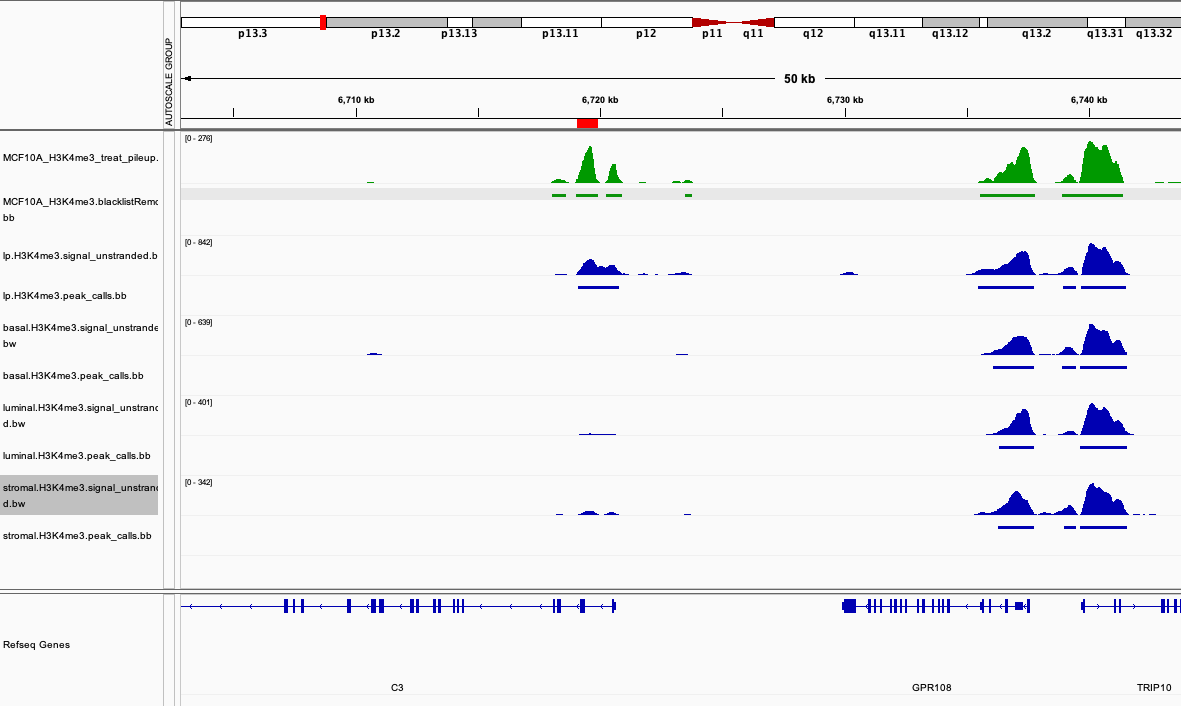
\includegraphics{./img/MCF10A-pLP-mBLS.png}

\begin{itemize}
\tightlist
\item
  \texttt{bedtools\ intersect\ -u\ -a\ \$\{MCF10A\_H3K4me3\}\ -b\ \$\{lp\_H3K4me3\}\ \textbar{}\ \ bedtools\ intersect\ -u\ -a\ stdin\ -b\ \ \{basal\_H3K4me3\}\ \textbar{}\ bedtools\ intersect\ -u\ -a\ stdin\ -b\ \$\{luminal\_H3K4me3\}\ \textbar{}\ bedtools\ intersect\ -u\ -a\ stdin\ -b\ \$\{stromal\_H3K4me3\}\ \ \textbar{}\ wc\ -l}

  \begin{itemize}
  \tightlist
  \item
    The command can be broken down into the following : \texttt{MCF10A\ Common\ with\ LP\ \textbar{}\ Common\ with\ Basal\ \textbar{}\ Common\ with\ Luminal\ \textbar{}\ Stromal}
  \end{itemize}
\end{itemize}

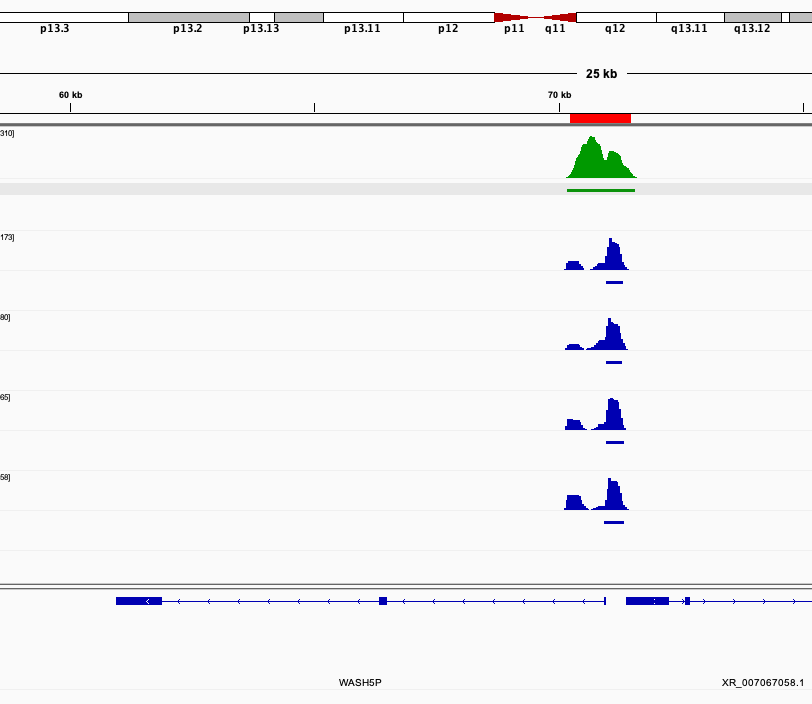
\includegraphics{./img/MCF10A-pLPMBLS.png}

\subsubsection{Step1E: Using Bedtools to compare binary conditions/models}\label{step1e-using-bedtools-to-compare-binary-conditionsmodels}

\begin{itemize}
\tightlist
\item
  We'll explore how to use bedtools to compare binary conditions and possible interpretations
\end{itemize}

\textbf{Code:}

\begin{verbatim}
###Shell###
condA_rep1=~/CourseData/EPI_data/module123/triplicates/peaks/CondA.Rep1_peaks.narrowPeak  
condB_rep1=~/CourseData/EPI_data/module123/triplicates/peaks/CondB.Rep1_peaks.narrowPeak
condA_rep2=~/CourseData/EPI_data/module123/triplicates/peaks/CondA.Rep2_peaks.narrowPeak  
condB_rep2=~/CourseData/EPI_data/module123/triplicates/peaks/CondB.Rep2_peaks.narrowPeak
condA_rep3=~/CourseData/EPI_data/module123/triplicates/peaks/CondA.Rep3_peaks.narrowPeak
condB_rep3=~/CourseData/EPI_data/module123/triplicates/peaks/CondB.Rep3_peaks.narrowPeak

bedtools intersect -u -a ${condA_rep1} -b ${condA_rep2} | wc -l
bedtools intersect -u -a ${condA_rep1} -b ${condB_rep2} | wc -l 
bedtools intersect -v -a ${condA_rep1} -b ${condA_rep2} | wc -l
bedtools intersect -v -a ${condA_rep1} -b ${condB_rep2} | wc -l

bedtools intersect -u -a ${condA_rep1} -b ${condA_rep2} ${condA_rep3} | wc -l

bedtools intersect -u -a ${condA_rep1} -b ${condA_rep2} ${condA_rep3} -f 0.5 -F 0.5 | wc -l

bedtools intersect -wao -a ${condA_rep1} -b ${condA_rep2} ${condA_rep3} | head
\end{verbatim}

\begin{itemize}
\tightlist
\item
  \texttt{bedtools\ intersect\ -u\ -a\ \$\{condA\_rep1\}\ -b\ \$\{condA\_rep2\}\ \textbar{}\ wc\ -l}

  \begin{itemize}
  \tightlist
  \item
    counting the number of condA\_rep1 peaks that intersect condA\_rep2
  \item
    returns \texttt{1191}
  \end{itemize}
\item
  \texttt{bedtools\ intersect\ -u\ -a\ \$\{condA\_rep1\}\ -b\ \$\{condB\_rep2\}\ \textbar{}\ wc\ -l}

  \begin{itemize}
  \tightlist
  \item
    counting the number of condA\_rep1 peaks that intersect condB\_rep2
  \item
    returns \texttt{1093}
  \end{itemize}
\item
  \texttt{bedtools\ intersect\ -v\ -a\ \$\{condA\_rep1\}\ -b\ \$\{condA\_rep2\}\ \textbar{}\ wc\ -l}

  \begin{itemize}
  \tightlist
  \item
    counting the number of condA\_rep1 peaks that do not intersect condA\_rep2
  \item
    return \texttt{50}
  \end{itemize}
\item
  \texttt{bedtools\ intersect\ -v\ -a\ \$\{condA\_rep1\}\ -b\ \$\{condB\_rep2\}\ \textbar{}\ wc\ -l}

  \begin{itemize}
  \tightlist
  \item
    counting the number of condA\_rep1 peaks that do not intersect condB\_rep2
  \item
    returns \texttt{148}
  \end{itemize}
\item
  as expected our replicates of matching conditions have more in common
\item
  \texttt{bedtools\ intersect\ -u\ -a\ \$\{condA\_rep1\}\ -b\ \$\{condA\_rep2\}\ \$\{condA\_rep3\}\ \textbar{}\ wc\ -l}

  \begin{itemize}
  \tightlist
  \item
    counting the number of condA\_rep1 peaks that intersect condA\_rep2 or condA\_rep3
  \end{itemize}
\item
  \texttt{bedtools\ intersect\ -wao\ -a\ \$\{condA\_rep1\}\ -b\ \$\{condA\_rep2\}\ \$\{condA\_rep3\}\ \textbar{}\ head}

  \begin{itemize}
  \tightlist
  \item
    specify \texttt{-wao} returns the original line of \texttt{\$\{condA\_rep1\}} and the element it intersects
  \item
    additionally adds an identify column for the database and number of base pairs overlapping
  \end{itemize}
\item
  \texttt{bedtools\ intersect\ -u\ -a\ \$\{condA\_rep1\}\ -b\ \$\{condA\_rep2\}\ \$\{condA\_rep3\}\ -f\ 0.5\ -F\ 0.5\ \textbar{}\ wc\ -l}

  \begin{itemize}
  \tightlist
  \item
    the flag \texttt{-f\ 0.5} adds the conditions that inte\#\#rsects are only counted when 50\% overlap of A occurs
  \item
    the flag \texttt{-F\ 0.5} adds the conditions that intersects are only counted when 50\% overlap of B occurs
  \item
    if we remove one of the flags, how does the number change?
  \item
    what if we wanted integer threshold instead of percentage?
  \end{itemize}
\item
  \texttt{bedtools\ intersect\ -wao\ -a\ \$\{condA\_rep1\}\ -b\ \$\{condA\_rep2\}\ \$\{condA\_rep3\}\ \textbar{}\ head}

  \begin{itemize}
  \tightlist
  \item
    specify \texttt{-wao} returns the original line of \texttt{\$\{condA\_rep1\}} and the element it intersects
  \item
    additionally adds an identify column for the database and number of base pairs overlapping
  \end{itemize}
\end{itemize}

\subsubsection{Step1F: Other useful bedtool functions}\label{step1f-other-useful-bedtool-functions}

\begin{itemize}
\tightlist
\item
  We'll highlight other useful bedtool applications.
\end{itemize}

\textbf{Code:}

\begin{verbatim}
###Shell###
MCF10A_H3K27ac=~/workspace/module123/peaks/MCF10A_H3K27ac_peaks.blacklistRemoved.narrowPeak
TSS=~/workspace/module123/resources/hg38v79_genes_tss_2000.bed

bedtools closest -a ${MCF10A_H3K27ac} -b ${TSS} -d | head

###
condA_peaks=~/CourseData/EPI_data/module123/triplicates/peaks/CondA.Rep1_peaks.narrowPeak
condB_peaks=~/CourseData/EPI_data/module123/triplicates/peaks/CondB.Rep1_peaks.narrowPeak

cat ${condA_peaks} ${condB_peaks} | sort -k1,1 -k2,2n | bedtools merge -i stdin > ~/workspace/module123/deeptools/merged_peaks.bed

####
methylation=~/workspace/module123/resources/example_methylation.bed

echo chr19 1 58617616 |\
sed 's/ /\t/g' |\
bedtools makewindows -w 50 -b stdin |\
awk 'BEGIN{{srand(1)}}{print $0"\t"rand()}' \
> ${methylation}

bedtools map -a ${MCF10A_H3K27ac} -b ${methylation} -c 4 -o median,count | head
\end{verbatim}

\begin{itemize}
\tightlist
\item
  \texttt{sed\ \textquotesingle{}s/\ /\textbackslash{}t/g\textquotesingle{}} replace a \texttt{} with \texttt{\textbackslash{}t}
\item
  \texttt{bedtools\ closest\ -a\ \$\{MCF10A\_H3K27ac\}\ -b\ \$\{TSS\}\ -d\ \textbar{}\ head}

  \begin{itemize}
  \tightlist
  \item
    Identifies features in fileB that are closes to fileA
  \item
    useful for mapping enhancers to their closest transcription start site
  \item
    \texttt{-d} will make the tool report the distance
  \item
    in our example, if the distance is zero the H3K27ac instead reflects an activated promoter.
  \end{itemize}
\item
  \texttt{cat\ \$\{condA\_rep1\}\ \$\{condA\_rep2\}\ \$\{condA\_rep3\}\ \textbar{}\ sort\ -k1,1\ -k2,2n\ \textbar{}\ bedtools\ merge\ -i\ stdin\ \textbar{}\ wc\ -l}

  \begin{itemize}
  \tightlist
  \item
    Pseudo code : \texttt{read\ peak\ files\ \textbar{}\ sort\ peak\ files\ \textbar{}\ merge\ peak\ files\ \textbar{}\ line\ count}
  \item
    \texttt{bedtools\ merge} takes elements specified in the input and merges the features if they intersect
  \item
    behaviour can be modified to require a certain mount overlap or bookended features
  \item
    compare how many peaks \texttt{cat\ \$\{condA\_rep1\}\ \$\{condA\_rep2\}\ \$\{condA\_rep3\}} starts off with
  \item
    following merge how many peaks are left?
  \end{itemize}
\item
  \texttt{echo\ chr19\textbackslash{}\textbackslash{}t1\textbackslash{}\textbackslash{}t58617616\ \textbar{}\ bedtools\ makewindows\ -w\ 50\ -b\ stdin\ \textbar{}\ awk\ \textquotesingle{}BEGIN\{srand(1);\}\{print\ \$0"\textbackslash{}t"rand()\}\textquotesingle{}\ \ \textgreater{}\ \$\{metylation\}}

  \begin{itemize}
  \tightlist
  \item
    Pseudo code : \texttt{simulate\ a\ bed\ file\ of\ chr19\ \textbar{}\ turn\ bedFile\ into\ 50bp\ bins\ \textbar{}\ add\ random\ float\ value}
  \item
    \texttt{echo\ chr19\textbackslash{}\textbackslash{}t1\textbackslash{}\textbackslash{}t58617616}

    \begin{itemize}
    \tightlist
    \item
      '\texttt{\textbackslash{}\textbackslash{}t} an escape character is uses to generate a tab
    \end{itemize}
  \item
    \texttt{bedtools\ makewindows\ -w\ 50\ -b\ stdin}

    \begin{itemize}
    \tightlist
    \item
      \texttt{-w\ 50} specifies our window size
    \item
      can alternatively use \texttt{-n} to specified how many windows we want to divide our bedFile into
    \end{itemize}
  \item
    \texttt{awk\ \textquotesingle{}BEGIN\{srand(1);\}\{print\ \$0"\textbackslash{}t"rand()\}\textquotesingle{}}

    \begin{itemize}
    \tightlist
    \item
      read our input (the 50bp window bed file of chr19) and generate a random float
    \item
      \texttt{srand(1)} set our seed number. Changing this will affect our pseudo random numbers
    \item
      \texttt{print\ \$0"\textbackslash{}t"rand()} as \texttt{awk} process line by line, print the current line (the windowed genomic coordiantes) and a random float number
    \end{itemize}
  \item
    \texttt{bedtools\ map\ -a\ \$\{MCF10A\_H3K27ac\}\ -b\ \$\{methylation\}\ -c\ 4\ -o\ median,count}

    \begin{itemize}
    \tightlist
    \item
      \texttt{bedtools\ map} apply a function summarizing the values of fileB that intersect fileA
    \item
      in our example for we're looking at the methylation of H3K27ac peaks
    \item
      \texttt{-c\ 4} indicates which columns from fileB we'd like to use
    \item
      \texttt{-o\ median,count} return the median of col 4 and coutn the number of elements from fileB that intersected the particular element from fileA
    \end{itemize}
  \end{itemize}
\end{itemize}

\subsubsection{Step2: Differential peaks utilizing triplicates and DiffBind}\label{step2-differential-peaks-utilizing-triplicates-and-diffbind}

\begin{itemize}
\tightlist
\item
  We'll perform analysis on mock MFC10A H3K4me3 data to get significant differential peaks for each condition. To do so, we'll utilizing the \texttt{diffBind} package in R
\end{itemize}

\textbf{Code :}

\begin{verbatim}
###R###
library(DiffBind)
setwd("/home/ubuntu")
samples <- read.csv("CourseData/EPI_data/module123/triplicates/triplicates.csv")
MCF10A <- dba(sampleSheet=samples)
MCF10A <- dba.count(MCF10A, bUseSummarizeOverlaps=TRUE)
dba.plotPCA(MCF10A, attributes=DBA_CONDITION,label=DBA_ID)
plot(MCF10A)
MCF10A <- dba.contrast(MCF10A, categories=DBA_CONDITION)

MCF10A <- dba.analyze(MCF10A, method=DBA_EDGER)

analyzed_peaks <- dba.report(MCF10A, method=DBA_EDGER, fold=1)

dba.plotMA(MCF10A, bXY=TRUE , method=DBA_EDGER, fold=1)

write.table(analyzed_peaks, file="workspace/module123/diffBind/differential_peaks.tsv", sep="\t", quote=F, row.names=F, col.names=F)
\end{verbatim}

\begin{itemize}
\tightlist
\item
  \texttt{library(DiffBind)}

  \begin{itemize}
  \tightlist
  \item
    we load R package \href{https://bioconductor.org/packages/release/bioc/html/DiffBind.html}{DiffBind}
  \end{itemize}
\item
  \texttt{setwd("/home/ubuntu")}

  \begin{itemize}
  \tightlist
  \item
    set our working directory
  \end{itemize}
\item
  \texttt{read.csv("CourseData/EPI\_data/module123/triplicates/triplicates.csv")}

  \begin{itemize}
  \tightlist
  \item
    read in our csv
  \item
    let's inspect the columns
  \end{itemize}
\item
  \texttt{MCF10A\ \textless{}-\ dba(sampleSheet=samples)}

  \begin{itemize}
  \tightlist
  \item
    read our samplesheet into the \texttt{dba} object that will be saved as \texttt{MCF10A}
  \end{itemize}
\item
  \texttt{MCF10A\ \textless{}-\ dba.count(MCF10A,\ bUseSummarizeOverlaps=TRUE)}

  \begin{itemize}
  \tightlist
  \item
    count the number of fragments that intersect with peaks
  \item
    \texttt{bUseSummarizeOverlaps=TRUE} indicates the counting module to be used. \texttt{SummarizeOverlaps} comes from \href{https://www.rdocumentation.org/packages/GenomicAlignments/versions/1.8.4/topics/summarizeOverlaps-methods}{GenomicAlignments}.
  \end{itemize}
\item
  \texttt{dba.plotPCA(MCF10A,\ attributes=DBA\_CONDITION,label=DBA\_ID)}

  \begin{itemize}
  \tightlist
  \item
    generate a principle component analysis using data from our object \texttt{MCF10A} where the annotations are \texttt{DBA\_CONDITION} and the labelling is \texttt{DBA\_ID}
  \end{itemize}
\item
  \texttt{plot(MCF10A)}

  \begin{itemize}
  \tightlist
  \item
    generate a heatmap with correlation and dendrogram
  \item
    should note the correlation is based on score of overlap and not pearson and spearman, should recalculate
  \end{itemize}
\item
  \texttt{MCF10A\ \textless{}-\ dba.contrast(MCF10A,\ categories=DBA\_CONDITION)}

  \begin{itemize}
  \tightlist
  \item
    declares what are the conditions for our differential groups
  \item
    \texttt{categories=DBA\_CONDITION} the category we want to compare
  \end{itemize}
\item
  \texttt{MCF10A\ \textless{}-\ dba.analyze(MCF10A,\ method=DBA\_EDGER)}

  \begin{itemize}
  \tightlist
  \item
    perform an analysis based on the \texttt{contrast} we previously established.
  \item
    \texttt{method=DBA\_EDGER}, analysis engine is a library called \texttt{edgeR}
  \item
    note for our specific example \texttt{deseq2} does not work. \texttt{Deseq2} has a built in check for variablity which our synthetic dataset is lacking
  \end{itemize}
\item
  \texttt{analyzed\_peaks\ \textless{}-\ dba.report(MCF10A,\ method=DBA\_EDGER,\ fold=1)}

  \begin{itemize}
  \tightlist
  \item
    report the peaks identified by \texttt{DBA\_EDGER} to be significant and have an absolute fold change \texttt{\textgreater{}1}
  \end{itemize}
\item
  \texttt{dba.plotMA(MCF10A,\ bXY=TRUE\ ,\ method=DBA\_EDGER,\ fold=1)}

  \begin{itemize}
  \tightlist
  \item
    generates Scatter plot
  \item
    \texttt{method=DBA\_EDGER} fetch results based on our previous analysis using \texttt{edgeR}
  \item
    \texttt{bXY=TRUE} produces a scatter plot, \texttt{FALSE} produces a MA plot
  \item
    \texttt{fold=1} report differential positions that meet fold change threshold
  \end{itemize}
\item
  \texttt{write.table(analyzed\_peaks,\ file="workspace/module123/diffBind/differential\_peaks.tsv",\ sep="\textbackslash{}t",\ quote=F,\ row.names=F,\ col.names=T)}

  \begin{itemize}
  \tightlist
  \item
    save our differential peaks to a TSV
  \item
    \texttt{sep="\textbackslash{}t"} the seperator to be used
  \item
    \texttt{col.names=T} include column names
  \item
    \texttt{row.names=F} include row names
  \item
    \texttt{quote=F} if we want to include quotations around values
  \end{itemize}
\end{itemize}

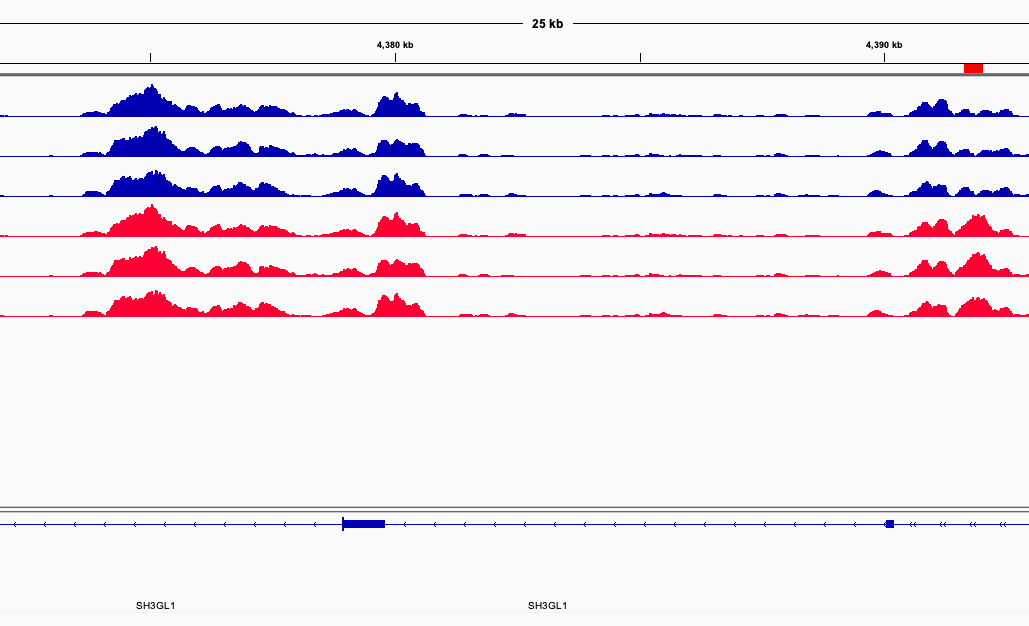
\includegraphics{./img/diffBind.png}

\subsubsection{Step3A: Differential peaks utilizing Fold change and significance - Merged peaks}\label{step3a-differential-peaks-utilizing-fold-change-and-significance---merged-peaks}

\begin{itemize}
\tightlist
\item
  Previously we performed differential analysis on triplicates, now let's explore how to do so on two samples.
\item
  We'll combine our two peak sets into an unified set.
\end{itemize}

\textbf{Code:}

\begin{verbatim}
###Shell###
condA_peaks=~/CourseData/EPI_data/module123/triplicates/peaks/CondA.Rep1_peaks.narrowPeak
condB_peaks=~/CourseData/EPI_data/module123/triplicates/peaks/CondB.Rep1_peaks.narrowPeak

cat ${condA_peaks} ${condB_peaks} | sort -k1,1 -k2,2n | bedtools merge -i stdin > ~/workspace/module123/edgeR/merged_peaks.bed
\end{verbatim}

\begin{itemize}
\tightlist
\item
  \texttt{cat\ \$\{condA\_peaks\}\ \$\{condB\_peaks\}\ \textbar{}\ sort\ -k1,1\ -k2,2n\ \textbar{}\ bedtools\ merge\ -i\ stdin\ \textgreater{}\ merged\_peaks.bed}

  \begin{itemize}
  \tightlist
  \item
    Pseudo code break down : \texttt{Read\ our\ peaks\ \textbar{}\ sort\ peaks\ coordinate\ wise\ \textbar{}\ merge\ peaks}
  \end{itemize}
\end{itemize}

\subsubsection{Step3B: Differential peaks utilizing Fold change and significance - Merged peaks}\label{step3b-differential-peaks-utilizing-fold-change-and-significance---merged-peaks}

\begin{itemize}
\tightlist
\item
  We'll combine our two peak sets into an unified set.
\end{itemize}

\textbf{Code:}

\begin{verbatim}
###Shell###
condA_peaks=~/CourseData/EPI_data/module123/triplicates/peaks/CondA.Rep1_peaks.narrowPeak
condB_peaks=~/CourseData/EPI_data/module123/triplicates/peaks/CondB.Rep1_peaks.narrowPeak
mkdir ~/workspace/module123/edgeR/
cat ${condA_peaks} ${condB_peaks} | sort -k1,1 -k2,2n | bedtools merge -i stdin > ~/workspace/module123/edgeR/merged_peaks.bed
\end{verbatim}

\begin{itemize}
\tightlist
\item
  \texttt{cat\ \$\{condA\_peaks\}\ \$\{condB\_peaks\}\ \textbar{}\ sort\ -k1,1\ -k2,2n\ \textbar{}\ bedtools\ merge\ -i\ stdin\ \textgreater{}\ merged\_peaks.bed}

  \begin{itemize}
  \tightlist
  \item
    Pseudo code break down : \texttt{Read\ our\ peaks\ \textbar{}\ sort\ peaks\ coordinate\ wise\ \textbar{}\ merge\ peaks}
  \end{itemize}
\end{itemize}

\subsubsection{Step3B: Differential peaks utilizing Fold change and significance - read counts per peak}\label{step3b-differential-peaks-utilizing-fold-change-and-significance---read-counts-per-peak}

\begin{itemize}
\tightlist
\item
  We'll derrive RPKM values per BAM for each peak in our peak set
\end{itemize}

\textbf{Code:}

\begin{verbatim}
###Shell###
peaks=~/workspace/module123/edgeR/merged_peaks.bed
condA_bam=~/workspace/module123/alignments/MCF10A_H3K4me3_chr19.CondA.Rep1.bam
condB_bam=~/workspace/module123/alignments/MCF10A_H3K4me3_chr19.CondB.Rep1.bam

condA_count=~/workspace/module123/edgeR/MCF10A_H3K4me3_chr19.CondA.Rep1.bed
condB_count=~/workspace/module123/edgeR/MCF10A_H3K4me3_chr19.CondB.Rep1.bed

bedtools intersect -a ${peaks} -b ${condA_bam} -c > ${condA_count}
bedtools intersect -a ${peaks} -b ${condB_bam} -c > ${condB_count}
\end{verbatim}

\begin{itemize}
\tightlist
\item
  \texttt{bedtools\ intersect\ -a\ \$\{peaks\}\ -b\ \$\{condA\_bam\}\ -c\ \textgreater{}\ \$\{condA\_count\}}

  \begin{itemize}
  \tightlist
  \item
    our intersect command is the same in principle but we're intersecting our peaks with a \texttt{BAM} file
  \item
    \texttt{-c} reports counts of our \texttt{BAM} that overlap our peaks
  \end{itemize}
\end{itemize}

\subsubsection{Step3C: Differential peaks utilizing Fold change and significance - EdgeR differential}\label{step3c-differential-peaks-utilizing-fold-change-and-significance---edger-differential}

\begin{itemize}
\tightlist
\item
  we'll read our data into \texttt{R} and perform a statistical analysis
\end{itemize}

\textbf{Code:}

\begin{verbatim}
\end{verbatim}

\#\#\#R\#\#\#
setwd(``/home/ubuntu'')
library(edgeR)
library(dplyr)

condA\textless-read.csv(``workspace/module123/edgeR/MCF10A\_H3K4me3\_chr19.CondA.Rep1.bed'',sep=`\t',col.names = c(``chr'', ``start'', ``end'',``MCF10A\_H3K4me3\_chr19.CondA.Rep1''),colClasses= c(``character'',``character'',``character'',``numeric''))
condB\textless-read.csv(``workspace/module123/edgeR/MCF10A\_H3K4me3\_chr19.CondB.Rep1.bed'',sep='\t',col.names = c(``chr'', ``start'', ``end'',``MCF10A\_H3K4me3\_chr19.CondB.Rep1''),colClasses= c(``character'',``character'',``character'',``numeric''))

peaks\textless-data.frame(
MCF10A\_H3K4me3\_chr19.CondA.Rep1=condA\(MCF10A_H3K4me3_chr19.CondA.Rep1,
    MCF10A_H3K4me3_chr19.CondB.Rep1=condB\)MCF10A\_H3K4me3\_chr19.CondB.Rep1
)
row.names(peaks)\textless-paste(condA\(chr,condA\)start,condA\$end,sep='\_')

edger\_dl \textless- DGEList(counts=peaks, group=1:2,lib.size=c(1131503,1266436))

edger\_tmm \textless- calcNormFactors(edger\_dl, method = ``TMM'')

bvc=0.1

edger\_et \textless- exactTest(edger\_tmm,dispersion=bvc\^{}2)

edger\_tp \textless- topTags(edger\_et, n=nrow(edger\_et\$table),adjust.method=``BH'')

de \textless- edger\_tp\$table \%\textgreater\% filter(FDR \textless{} 0.01) \%\textgreater\% filter(logFC \textgreater=1 \textbar{} logFC \textless=-1)

write.table(de, file=``workspace/module123/edgeR/differential\_peaks\_edger.tsv'', sep=``\t", quote=F, row.names=F, col.names=F)

\begin{verbatim}
- `condA<-read.csv("workspace/module123/edgeR/MCF10A_H3K4me3_chr19.CondA.Rep1.bed",sep='\t',col.names = c("chr", "start", "end","MCF10A_H3K4me3_chr19.CondA.Rep1"),colClasses= c("character","character","character","numeric"))`
    - `read.csv` read the `CSV` file into a `data.frame`
    - `sep='\t'` specify the delimiter
    - `col.names = c("chr", "start", "end","MCF10A_H3K4me3_chr19.CondA.Rep1")` set our column names
    - `colClasses= c("character","character","character","numeric")` indicate with column are what datatypes
- `peaks<-data.frame(MCF10A_H3K4me3_chr19.CondA.Rep1=condA$MCF10A_H3K4me3_chr19.CondA.Rep1,MCF10A_H3K4me3_chr19.CondB.Rep1=condB$MCF10A_H3K4me3_chr19.CondB.Rep1)`
    - make a new data.frame using our two columns from condA and condB
- `row.names(peaks)<-paste(peaks$chr,peaks$start,peaks$end,sep='_')`
    - edit row names to be match genomic coordinates
    - ``row.names(peaks)<-` indicate we want to overwrite exist row names
    - `paste(peaks$chr,peaks$start,peaks$end,sep='_')` we want to concatenate our `chr`,`start` and `end` with `_` as a seperator
- `edger_dl <- DGEList(counts=peaks, group=1:2,lib.size=c(1131503,1266436))`
    - `DGEList(counts=peaks_clean, group=1:2)` read in our `peak_clean` data.frame
    - `group=1:2` identify which groups we want to contrast
    - `lib.size=c(1131503,1266436)` library size for the two conditions
- `edger_tmm <- calcNormFactors(edger_dl, method = "TMM")` calculate the normalization factor to scale library sizes
- `bvc=0.01` Set the `square-rootdispersion`. according to edgeR documentation: `from well-controlled experiments are 0.4 for human data, 0.1 for data on genetically identical model organisms or 0.01 for technical replicates`
- `edger_et <- exactTest(edger_dl,dispersion=bcv^2)`
    - calculate `FC` and `Pvalue` per row
- `edger_tp <- topTags(edger_et, n=nrow(edger_et$table),adjust.method="BH")`
    - calcualte `FDR` via Benjamini-Hochberg
- `de <- edger_tp$table %>% filter(FDR < 0.01) %>% filter(logFC >=1 | logFC <=-1)`
    - `filter(FDR < 0.01)` filter for significant peaks
    - `filter(logFC >=1 | logFC <=-1)` filter for peaks with appropriate fold change
- `write.table(de, file="workspace/module123/edgeR/differential_peaks_edger.tsv", sep="\t", quote=F, row.names=F, col.names=F)`
    - save files
<img src="https://github.com/bioinformaticsdotca/EPI_2023/blob/module123/module123_images/edger.png?raw=true" alt="Region" width="750" />
\end{verbatim}

\subsection{Server resources}\label{server-resources-2}

\subsubsection{QC Resources}\label{qc-resources-2}

\begin{verbatim}
###TSS+/-2kb
mkdir workspace/module123/qc
wget https://www.bcgsc.ca/downloads/esu/touchdown/hg38v79_genes_tss_2000.bed -O workspace/module123/resources/hg38v79_genes_tss_2000.bed

sort -k1,1 -k2,2n workspace/module123/resources/hg38v79_genes_tss_2000.bed > tmp
mv tmp workspace/module123/resources/hg38v79_genes_tss_2000.bed

###Enhancer liftover
wget https://www.bcgsc.ca/downloads/esu/touchdown/encode_enhancers_liftover.bed -O workspace/module123/resources/encode_enhancers_liftover.bed

###Blacklist
wget https://www.encodeproject.org/files/ENCFF356LFX/@@download/ENCFF356LFX.bed.gz -O ~/workspace/module123/resources/hg38_blacklist.bed.gz

gunzip ~/workspace/module123/resources/hg38_blacklist.bed.gz
\end{verbatim}

\begin{itemize}
\tightlist
\item
  \texttt{hg38v79\_genes\_tss\_2000.bed}

  \begin{itemize}
  \tightlist
  \item
    Generated by downloading Ensemblv79 GTF convert to Bed +/-2kb of TSS. See \url{https://www.biostars.org/p/56280/}
  \end{itemize}
\item
  \texttt{encode\_enhancers\_liftover.bed}

  \begin{itemize}
  \tightlist
  \item
    download various \href{https://egg2.wustl.edu/roadmap/data/byFileType/chromhmmSegmentations/ChmmModels/coreMarks/jointModel/final/}{ChroHMM state7} and merge
  \end{itemize}
\end{itemize}

\subsubsection{Encode Bed}\label{encode-bed-2}

\begin{verbatim}
ls ~/CourseData/EPI_data/module123/encode_bed
basal.H3K27ac.peak_calls.bed
basal.H3K27me3.peak_calls.bed
basal.H3K4me1.peak_calls.bed
basal.H3K4me3.peak_calls.bed
lp.H3K27ac.peak_calls.bed
lp.H3K27me3.peak_calls.bed
lp.H3K4me1.peak_calls.bed
lp.H3K4me3.peak_calls.bed
luminal.H3K27ac.peak_calls.bed
luminal.H3K27me3.peak_calls.bed
luminal.H3K4me1.peak_calls.bed
luminal.H3K4me3.peak_calls.bed
stromal.H3K27ac.peak_calls.bed
stromal.H3K27me3.peak_calls.bed
stromal.H3K4me1.peak_calls.bed
stromal.H3K4me3.peak_calls.bed
\end{verbatim}

\begin{itemize}
\tightlist
\item
  \url{https://epigenomesportal.ca/tracks/CEEHRC/hg38/}
\item
  Breast Basal CEMT0035
\item
  Breast Stromal CEMT0036
\item
  Breast Luminal CEMT0037
\item
  Breast Luminal Progenitor CEMT0038
  \#\#\#\# Encode BigWig
\end{itemize}

\begin{verbatim}
ls ~/CourseData/EPI_data/module123/encode_bigWig
basal.H3K27ac.signal_unstranded.bigWig
basal.H3K27me3.signal_unstranded.bigWig
basal.H3K4me1.signal_unstranded.bigWig
basal.H3K4me3.signal_unstranded.bigWig
lp.H3K27ac.signal_unstranded.bigWig
lp.H3K27me3.signal_unstranded.bigWig
lp.H3K4me1.signal_unstranded.bigWig
lp.H3K4me3.signal_unstranded.bigWig
luminal.H3K27ac.signal_unstranded.bigWig
luminal.H3K27me3.signal_unstranded.bigWig
luminal.H3K4me1.signal_unstranded.bigWig
luminal.H3K4me3.signal_unstranded.bigWig
stromal.H3K27ac.signal_unstranded.bigWig
stromal.H3K27me3.signal_unstranded.bigWig
stromal.H3K4me1.signal_unstranded.bigWig
stromal.H3K4me3.signal_unstranded.bigWig
\end{verbatim}

\begin{itemize}
\tightlist
\item
  \url{https://epigenomesportal.ca/tracks/CEEHRC/hg38/}
\item
  Breast Basal CEMT0035
\item
  Breast Stromal CEMT0036
\item
  Breast Luminal CEMT0037
\item
  Breast Luminal Progenitor CEMT0038
  \#\#\#\# MCF10A Fastq
\end{itemize}

\begin{verbatim}
ls ~/CourseData/EPI_data/module123/fastq
MCF10A.ATAC.chr19.R1.fastq.gz
MCF10A.ATAC.chr19.R2.fastq.gz
MCF10A.H3K27ac.chr19.R1.fastq.gz
MCF10A.H3K27ac.chr19.R2.fastq.gz
MCF10A.H3K27me3.chr19.R1.fastq.gz
MCF10A.H3K27me3.chr19.R2.fastq.gz
MCF10A.H3K4me3.chr19.R1.fastq.gz
MCF10A.H3K4me3.chr19.R2.fastq.gz
MCF10A.Input.chr19.R1.fastq.gz
MCF10A.Input.chr19.R2.fastq.gz
\end{verbatim}

\begin{itemize}
\tightlist
\item
  MCF10A histone marks and input come courtesy of Dr.Hirst
\item
  ATACseq data originates from \href{https://www.ncbi.nlm.nih.gov/geo/query/acc.cgi?acc=GSM6431322}{GSM6431322}
  \#\#\#\# Triplicates
\end{itemize}

\begin{verbatim}
CourseData/EPI_data/module123/triplicates/triplicates.csv

CourseData/EPI_data/module123/triplicates/alignments:
MCF10A_H3K4me3_chr19.CondA.Rep1.bam      MCF10A_H3K4me3_chr19.CondB.Rep2.bam      MCF10A_input_chr19.CondA.Rep3.bam
MCF10A_H3K4me3_chr19.CondA.Rep1.bam.bai  MCF10A_H3K4me3_chr19.CondB.Rep2.bam.bai  MCF10A_input_chr19.CondA.Rep3.bam.bai
MCF10A_H3K4me3_chr19.CondA.Rep2.bam      MCF10A_H3K4me3_chr19.CondB.Rep3.bam      MCF10A_input_chr19.CondB.Rep1.bam
MCF10A_H3K4me3_chr19.CondA.Rep2.bam.bai  MCF10A_H3K4me3_chr19.CondB.Rep3.bam.bai  MCF10A_input_chr19.CondB.Rep1.bam.bai
MCF10A_H3K4me3_chr19.CondA.Rep3.bam      MCF10A_input_chr19.CondA.Rep1.bam        MCF10A_input_chr19.CondB.Rep2.bam
MCF10A_H3K4me3_chr19.CondA.Rep3.bam.bai  MCF10A_input_chr19.CondA.Rep1.bam.bai    MCF10A_input_chr19.CondB.Rep2.bam.bai
MCF10A_H3K4me3_chr19.CondB.Rep1.bam      MCF10A_input_chr19.CondA.Rep2.bam        MCF10A_input_chr19.CondB.Rep3.bam
MCF10A_H3K4me3_chr19.CondB.Rep1.bam.bai  MCF10A_input_chr19.CondA.Rep2.bam.bai    MCF10A_input_chr19.CondB.Rep3.bam.bai

CourseData/EPI_data/module123/triplicates/bigWig:
CondA.Rep1.bw  CondA.Rep2.bw  CondA.Rep3.bw  CondB.Rep1.bw  CondB.Rep2.bw  CondB.Rep3.bw

CourseData/EPI_data/module123/triplicates/peaks:
CondA.Rep1_peaks.narrowPeak  CondA.Rep3_peaks.narrowPeak  CondB.Rep2_peaks.narrowPeak
CondA.Rep2_peaks.narrowPeak  CondB.Rep1_peaks.narrowPeak  CondB.Rep3_peaks.narrowPeak
\end{verbatim}

\begin{itemize}
\tightlist
\item
  triplicates were generated from MCF10A\_H3K4me3 by choosing a list of exclusive peaks for condA and condB and subsampling replicates accordingly
\end{itemize}

Congratulations! You have completed Lab 3!

\chapter{Module 4: Whole-Genome Bisulfite Sequencing and Analysis}\label{module-4-whole-genome-bisulfite-sequencing-and-analysis}

\section{Lecture}\label{lecture-3}

\section{Lab}\label{lab-3}

\subsection{1. Introduction}\label{introduction}

\subsubsection{Description of the lab:}\label{description-of-the-lab}

This module will cover the basics of Whole Genome Bisulfite-Sequencing (WGBS) data analysis including data visualization in IGV.

\subsubsection{Objectives:}\label{objectives}

\begin{enumerate}
\def\labelenumi{\arabic{enumi})}
\tightlist
\item
  Learn how to align WGBS data using \texttt{Bismark}
\item
  Learn how to generate a methylation profile with \texttt{Bismark}
\item
  Learn how to open alignments and methylation profiles in the \texttt{IGV} genome browser
\item
  Learn how to perform a basic differential methylation analysis with \texttt{MethylKit}
\end{enumerate}

\subsubsection{Local software that we will use:}\label{local-software-that-we-will-use}

Before you begin, make sure you have the following programs ready in your local computer:

\begin{itemize}
\tightlist
\item
  A connection to the \texttt{EPI\_2021} AWS instance
\item
  An internet browser
\item
  IGV
\item
  R (or RStudio), \emph{optional}
\end{itemize}

\begin{center}\rule{0.5\linewidth}{0.5pt}\end{center}

\subsection{2. Mapping Tutorial}\label{mapping-tutorial}

\subsubsection{2.1 Getting Started}\label{getting-started}

\paragraph{Prepare Directory for the Lab}\label{prepare-directory-for-the-lab}

\begin{Shaded}
\begin{Highlighting}[]
\FunctionTok{mkdir} \AttributeTok{{-}p}\NormalTok{ \textasciitilde{}/workspace/module4}
\BuiltInTok{cd}\NormalTok{ \textasciitilde{}/workspace/module4}
\end{Highlighting}
\end{Shaded}

\paragraph{Save Genome Location}\label{save-genome-location}

\begin{Shaded}
\begin{Highlighting}[]
\VariableTok{GENOME}\OperatorTok{=}\NormalTok{\textasciitilde{}/CourseData/EPI\_data/module4/Homo\_sapiens.GRCh38.chr19}
\BuiltInTok{export} \VariableTok{GENOME}
\end{Highlighting}
\end{Shaded}

This will define a variable \texttt{\$GENOME} that will simplify future commands.

\begin{center}\rule{0.5\linewidth}{0.5pt}\end{center}

\subsubsection{Locate the Data for the Workshop}\label{locate-the-data-for-the-workshop}

\begin{Shaded}
\begin{Highlighting}[]
\VariableTok{WGBS\_DATA}\OperatorTok{=}\NormalTok{\textasciitilde{}/CourseData/EPI\_data/module4/data}
\BuiltInTok{export} \VariableTok{WGBS\_DATA}
\end{Highlighting}
\end{Shaded}

This will define a variable \texttt{\$WGBS\_DATA} that will simplify future commands.

\paragraph{Check the Files}\label{check-the-files}

Type the following command: \texttt{ls\ \$WGBS\_DATA}, what do you see?

You should see something similar to this

\begin{verbatim}
WGBS.A34002.137160.chr19.1.fastq.gz
WGBS.A34002.137160.chr19.2.fastq.gz
WGBS.A34002.137487.chr19.1.fastq.gz
WGBS.A34002.137487.chr19.2.fastq.gz
WGBS.A34002.137488.chr19.1.fastq.gz
WGBS.A34002.137488.chr19.2.fastq.gz
\end{verbatim}

These are the files that will be used for the workshop. They contain a subset of WGBS reads from CEMT sample \texttt{CEMT0007}, which is a mammary gland epithelial cell line \href{https://ega-archive.org/datasets/EGAD00001000685}{(more information here)}.

\textbf{What do the ``.1'' and ``.2'' in the file names mean?}

They represent the \texttt{read1} and \texttt{read2} of the paired end reads.

\begin{center}\rule{0.5\linewidth}{0.5pt}\end{center}

\subsubsection{2.2 Map Data using Bismark}\label{map-data-using-bismark}

We will now process and map the reads using the Bismark WGBS aligner \href{https://www.bioinformatics.babraham.ac.uk/projects/bismark/}{(more info here)}.

\paragraph{Map the first dataset using Bismark}\label{map-the-first-dataset-using-bismark}

To simplify the work, we will process the datasets one at a time. To align the first dataset, do the following:

\begin{verbatim}
cd ~/workspace/module4
bismark --multicore 4 --bowtie2 $GENOME/genome/bismark_index \
    -1 $WGBS_DATA/WGBS.A34002.137160.chr19.1.fastq.gz -2 $WGBS_DATA/WGBS.A34002.137160.chr19.2.fastq.gz
    
\end{verbatim}

\textbf{What do all the options in the command mean?} (Hint check the help by using \texttt{bismark\ -\/-help})

The \texttt{-\/-multicore\ 4} option is to do multithreaded processing to improve speed.

The \texttt{-\/-bowtie2} option is to use the mapping algorithm from bowtie2.

The \texttt{\$GENOME/genome/bismark\_index} specifies the location of the index for the reference genome to use. This uses the \texttt{\$GENOME} variable we defined previously.

The \texttt{-1\ \$WGBS\_DATA/WGBS.A34002.137160.chr19.1.fastq.gz} specifies the location of read 1. Idem for \texttt{-2} which specifies read 2. This uses the \texttt{\$WGBS\_DATA} variable we defined previously.

For more details, please refer to the Bismark \href{http://www.bioinformatics.babraham.ac.uk/projects/bismark/Bismark_User_Guide.pdf}{user guide}.

\begin{center}\rule{0.5\linewidth}{0.5pt}\end{center}

This step will take a few minutes to run for this reduced dataset. A dataset spanning a full genome will take \emph{several hours}.

For your own datasets, make sure you have enough computing walltime to run the alignment.

\textbf{While you wait for the results, ask any questions you have up to this point to the instructors.}

\paragraph{Check files}\label{check-files}

At the end of the alignment, you should have the following files saved into your workshop folder:

\texttt{\{:output\}\ WGBS.A34002.137160.chr19.1\_bismark\_bt2\_pe.bam\ \ WGBS.A34002.137160.chr19.1\_bismark\_bt2\_PE\_report.txt}

Bismark offers a tool to generate an interactive HTML report for each sample, which we can now run to obtain the summary for our first sample.

\begin{verbatim}
bismark2report
\end{verbatim}

This will produce an additional file called: \texttt{WGBS.A34002.137160.chr19.1\_bismark\_bt2\_PE\_report.html}.

Let's look at the report. We can read the text file directly on the command line:

\begin{verbatim}
less WGBS.A34002.137160.chr19.1_bismark_bt2_PE_report.txt
\end{verbatim}

Or open the HTML report using your internet browser and the IP address of your AWS instance. Just click on the link to the HTML report and it should open.

\textbf{What was the mapping efficiency? What percent of C's were methylated in CpG context? }

According to the report:

\begin{verbatim}
...
Mapping efficiency:     92.4% 
...
C methylated in CpG context:    57.4%
C methylated in CHG context:    0.6%
C methylated in CHH context:    0.5%
C methylated in unknown context (CN or CHN):    3.5%
...
\end{verbatim}

You can also look at plot the \texttt{Cytosine\ Methylation} section in the interactive HTML report.

Close the report by pressing \texttt{q}.

\begin{center}\rule{0.5\linewidth}{0.5pt}\end{center}

\paragraph{Prepare files for loading in IGV}\label{prepare-files-for-loading-in-igv}

We need to sort the \texttt{bam} file and prepare an index so we will be able to load it in IGV. We will use the program \texttt{samtools} for this.

\begin{verbatim}
samtools sort WGBS.A34002.137160.chr19.1_bismark_bt2_pe.bam -o WGBS.A34002.137160.chr19.1_bismark_bt2_pe_sorted.bam 
samtools index WGBS.A34002.137160.chr19.1_bismark_bt2_pe_sorted.bam
\end{verbatim}

\paragraph{Check Files}\label{check-files-1}

At the end, you should have the following files:

\begin{verbatim}
WGBS.A34002.137160.chr19.1_bismark_bt2_pe_sorted.bam
WGBS.A34002.137160.chr19.1_bismark_bt2_pe.bam         
WGBS.A34002.137160.chr19.1_bismark_bt2_pe_sorted.bam.bai
WGBS.A34002.137160.chr19.1_bismark_bt2_PE_report.txt
\end{verbatim}

\begin{center}\rule{0.5\linewidth}{0.5pt}\end{center}

\subsubsection{2.3 Repeat Alignment for All Datasets}\label{repeat-alignment-for-all-datasets}

\textbf{How would you repeat the alignment with the other datasets?}

This is the command to run bismark on the two other samples:

\begin{verbatim}
cd ~/workspace/module4

bismark --multicore 4 --bowtie2 $GENOME/genome/bismark_index \
    -1 $WGBS_DATA/WGBS.A34002.137487.chr19.1.fastq.gz -2 $WGBS_DATA/WGBS.A34002.137487.chr19.2.fastq.gz
    
bismark --multicore 4 --bowtie2 $GENOME/genome/bismark_index \
    -1 $WGBS_DATA/WGBS.A34002.137488.chr19.1.fastq.gz -2 $WGBS_DATA/WGBS.A34002.137488.chr19.2.fastq.gz
    
\end{verbatim}

Remember, for the command to work, both \texttt{\$GENOME} and \texttt{\$WGBS\_DATA} need to be defined.

Also, if you want to generate the HTML reports, you can run \texttt{bismark2report}. Bismark also has a ``summary'' that produces a report for all samples (\texttt{bismark2summary}), we can run both by doing the following:

\begin{verbatim}
bismark2report ; bismark2summary
\end{verbatim}

After checking the reports, we can run the commands to prepare the samples for IGV (sort and index):

\begin{verbatim}
samtools sort  WGBS.A34002.137487.chr19.1_bismark_bt2_pe.bam -o WGBS.A34002.137487.chr19.1_bismark_bt2_pe_sorted.bam
samtools index WGBS.A34002.137487.chr19.1_bismark_bt2_pe_sorted.bam

samtools sort  WGBS.A34002.137488.chr19.1_bismark_bt2_pe.bam -o WGBS.A34002.137488.chr19.1_bismark_bt2_pe_sorted.bam
samtools index WGBS.A34002.137488.chr19.1_bismark_bt2_pe_sorted.bam
\end{verbatim}

\begin{center}\rule{0.5\linewidth}{0.5pt}\end{center}

\subsubsection{2.4 Load Data and Explore using IGV}\label{load-data-and-explore-using-igv}

While you wait for the previous steps to finish executing, it is a good idea to begin exploring the alignments.

\paragraph{Copy Files to Your Local Computer to View in IGV}\label{copy-files-to-your-local-computer-to-view-in-igv}

Retrieve the files called \texttt{WGBS.A34002.137160.chr19.1\_bismark\_bt2\_pe\_sorted.bam} and \texttt{WGBS.A34002.137160.chr19.1\_bismark\_bt2\_pe\_sorted.bam.bai} from the server using your internet browser and the IP address of your AWS instance.

Optionally, if you are not using Putty (i.e.~if you are using a Linux or Mac computer) you can also retrieve the files directly using the terminal and \texttt{scp} using the commands below.

\textbf{Optional download option} (click here)

\begin{verbatim}
scp -i CBW.pem ubuntu@00.00.00.0:~/workspace/module4/WGBS.A34002.137160.chr19.1_bismark_bt2_pe_sorted.bam .
scp -i CBW.pem ubuntu@00.00.00.0:~/workspace/module4/WGBS.A34002.137160.chr19.1_bismark_bt2_pe_sorted.bam.bai .
\end{verbatim}

Remember that for the commands above to work, you need to be in the directory with the \texttt{CBW.pem} (or \texttt{CBW.cer}) file you downloaded from AWS when creating your instance.

\paragraph{Launch IGV on your computer}\label{launch-igv-on-your-computer}

If you haven't installed it yet, please get it here \href{http://software.broadinstitute.org/software/igv/download}{IGV download}.

Make sure that the human genome is selected in the top left corner. It should read: \textbf{Human (hg38)}.

Load your \textbf{sorted} \texttt{bam} file in IGV using \texttt{File\ -\textgreater{}\ Load\ from\ file}. \emph{For this to work, you need to have the index file (\texttt{.bai}) in the same location as the \texttt{bam} file.}

Now go to the following location:

\begin{verbatim}
chr19:43,375,889-45,912,052
\end{verbatim}

And zoom in until you see something.

For instance, try the following window:

\begin{verbatim}
chr19:44,527,387-44,536,873
\end{verbatim}

You should see something like this:

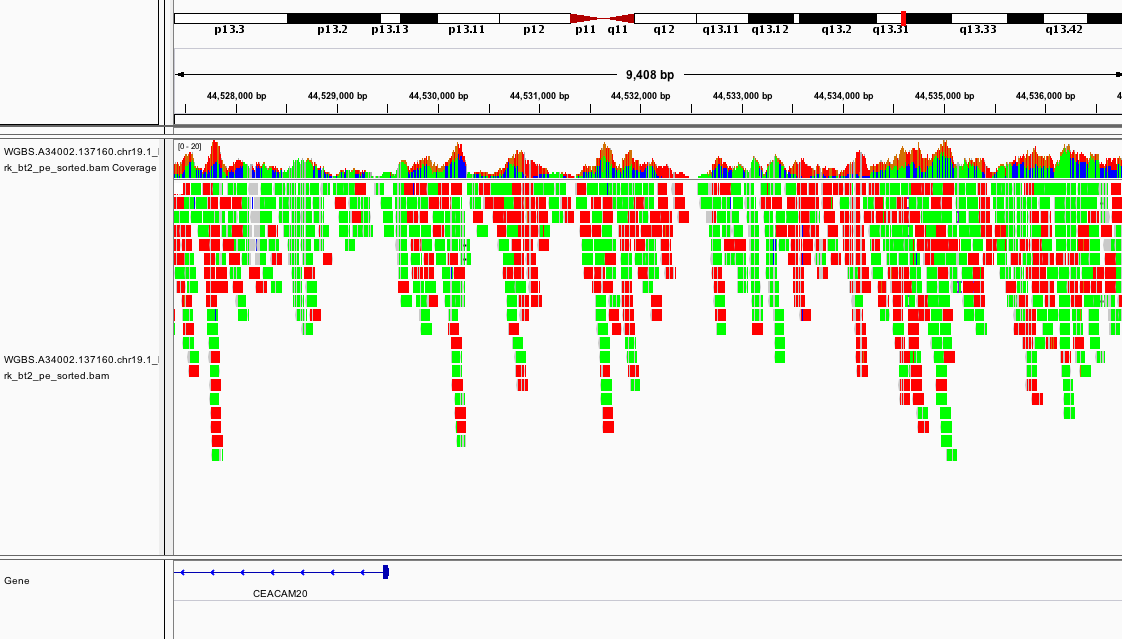
\includegraphics{./img/region2.png}

\emph{If it looks different, can you change the way the colors are displayed?}

\emph{Which section of which chromosome is covered by this dataset?}

\emph{Can you see any interesting patterns in the coverage?}

\begin{center}\rule{0.5\linewidth}{0.5pt}\end{center}

\subsubsection{2.5 Generate Methylation Profiles}\label{generate-methylation-profiles}

So far we have only mapped the reads using Bismark. We can generate methylation profiles using the following command:

\begin{verbatim}
cd ~/workspace/module4

bismark_methylation_extractor --cytosine_report WGBS.A34002.137160.chr19.1_bismark_bt2_pe.bam --genome_folder $GENOME/genome/bismark_index
\end{verbatim}

The \texttt{-\/-cytosine\_report} option creates a \texttt{CpG\_report} table summarizing key data for each \texttt{CG} position in the genome, which will be useful later (see \hyperref[r_dss_import]{section 4.2}).

\textbf{How would you do the same for the other replicates?}

These are the commands that you should use:

\begin{verbatim}
cd ~/workspace/module4

bismark_methylation_extractor --cytosine_report WGBS.A34002.137487.chr19.1_bismark_bt2_pe.bam --genome_folder $GENOME/genome/bismark_index
bismark_methylation_extractor --cytosine_report WGBS.A34002.137488.chr19.1_bismark_bt2_pe.bam --genome_folder $GENOME/genome/bismark_index
\end{verbatim}

\begin{center}\rule{0.5\linewidth}{0.5pt}\end{center}

Download \emph{all} the files produced so far to your local computer using your internet browser.

\textbf{While you wait for all the steps and downloads to finish, you can ask the instructors any questions you might have up until this point.}

\begin{center}\rule{0.5\linewidth}{0.5pt}\end{center}

Load all the downloaded files in IGV using \texttt{File\ -\textgreater{}\ Load\ from\ file}.

\textbf{Please be aware that if you just try to open all your files on IGV you might get a warning/error message mentioning that you are trying to open an unsorted BAM. If that is the case, ignore the message, but make sure that you are opening the \texttt{sorted.bam} so you can visualize your results.}

At this point, if you load the region \texttt{chr19:44,527,387-44,536,873} you should see something like

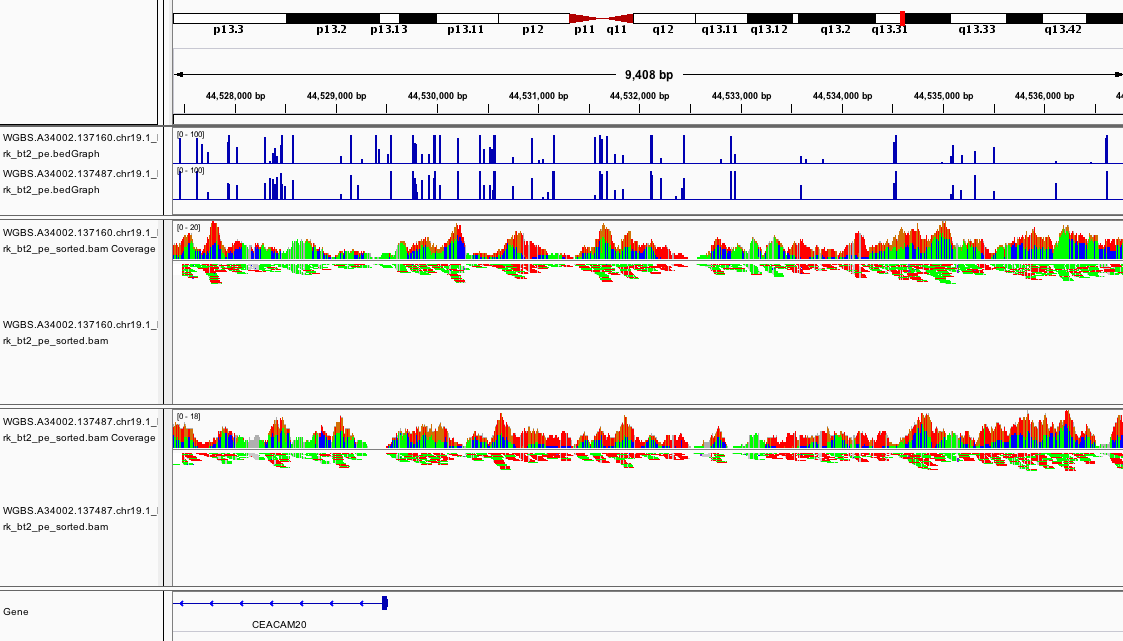
\includegraphics{./img/region2_full.png}

This promoter looks to be hypomethylated.

\emph{Can you find a promoter that is hypermethylated?}

How about \texttt{chr19:45,637,715-45,657,380}?

\emph{How would you look for a CpG island using this view of the data?}

\begin{center}\rule{0.5\linewidth}{0.5pt}\end{center}

\subsection{3. Differential Methylation Analysis in MethylKit}\label{differential-methylation-analysis-in-methylkit}

The following section will use the Bioconductor package \texttt{methylKit} to do a differential methylation analysis.
You can do it in your own computer (if you have installed \texttt{R} and \texttt{methylKit}) or in the AWS instance.

To install \texttt{methylKit} locally on your computer, make sure you have a recent version of \texttt{R} and
follow the instructions in this \href{https://bioconductor.org/packages/release/bioc/html/methylKit.html}{page}.

\begin{center}\rule{0.5\linewidth}{0.5pt}\end{center}

\subsubsection{3.1 Load R and MethylKit}\label{load-r-and-methylkit}

If you are working in AWS, you will need to load \texttt{R}. The image we provide already has the libraries we need.

To launch \texttt{R} simply type the following to your terminal:

\begin{verbatim}
cd ~/workspace/module4
R
\end{verbatim}

If you did this properly, the following message will be displayed and your prompt will change from \textbf{\texttt{ubuntu@ip-00-00-00-0:\textasciitilde{}/workspace/module4\$}} to \textbf{\texttt{\textgreater{}}}:

```\{:output\}
R version 4.2.3 (2023-03-15) -- ``Shortstop Beagle''
Copyright (C) 2023 The R Foundation for Statistical Computing
Platform: x86\_64-pc-linux-gnu (64-bit)
\ldots{}

\begin{verbatim}

Once you have successfully launched `R`, you can load `methylKit` with the following command: 

```{}
library("methylKit") 
\end{verbatim}

\begin{center}\rule{0.5\linewidth}{0.5pt}\end{center}

\subsubsection{3.2 Import the Alignment Data into methylKit}\label{import-the-alignment-data-into-methylkit}

\paragraph{Process Bismark Alignments}\label{process-bismark-alignments}

To read the alignment data into \texttt{methylKit}, run the following command:

\begin{verbatim}
methRaw.160 = processBismarkAln( location = "WGBS.A34002.137160.chr19.1_bismark_bt2_pe_sorted.bam",
                         sample.id="A34002.137160", assembly="hg38", 
                         read.context="CpG", save.folder="methylkit")
\end{verbatim}

This command will import the data into a format that is readable by \texttt{methylKit}. At the same time, it will save two files under the \texttt{methylkit} directory with the information so that it is easy to load again at any time:

\begin{verbatim}
methylkit/A34002.137160_CpG_conversionStats.txt
methylkit/A34002.137160_CpG.txt
\end{verbatim}

If everything goes well and you see the files, do the same for the other two samples:

\begin{verbatim}
methRaw.487 = processBismarkAln( location = "WGBS.A34002.137487.chr19.1_bismark_bt2_pe_sorted.bam",
                         sample.id="A34002.137487", assembly="hg38", 
                         read.context="CpG", save.folder="methylkit")
                         
methRaw.488 = processBismarkAln( location = "WGBS.A34002.137488.chr19.1_bismark_bt2_pe_sorted.bam",
                         sample.id="A34002.137488", assembly="hg38", 
                         read.context="CpG", save.folder="methylkit")
\end{verbatim}

\begin{center}\rule{0.5\linewidth}{0.5pt}\end{center}

\paragraph{Create a MethylKit Object}\label{create-a-methylkit-object}

Now that all the samples have been read with \texttt{methylKit}, you can create a file list to make it easier to load the full dataset as a \texttt{methylkit} object. For the purposes of this tutorial, we will consider that samples belong to two experimental groups: \texttt{A34002.137160} as the control group (treatment = 0) and \texttt{A34002.137487} \& \texttt{A34002.137488} as the treatment group (treatment = 1). We use the \texttt{methRead()} function to create our object, as shown below:

\begin{verbatim}
file.list = list( file.path("methylkit", "A34002.137160_CpG.txt"),
                  file.path("methylkit", "A34002.137487_CpG.txt"),
                  file.path("methylkit", "A34002.137488_CpG.txt") )

myobj = methRead(file.list,
           sample.id=list("A34002.137160","A34002.137487","A34002.137488"),
           assembly="hg38",
           treatment=c(0,1,1),
           context="CpG",
           mincov = 10
           )
\end{verbatim}

\textbf{What do all the options in the \texttt{methRead()} command mean?}

\begin{itemize}
\item
  \texttt{file.list} object points to the location of the input data in a MethylKit format.
\item
  \texttt{sample.id} points to a list with the appropriate sample name for each file.
\item
  \texttt{assembly} specifies which build of the human reference genome is used.
\item
  \texttt{treatment} specifies which sample belongs to each experimental group.
\item
  \texttt{context} specifies the methylation context.
\item
  \texttt{mincov} specifies the minimum coverage required to be included in the object.
\end{itemize}

For more details, please refer to the MethylKit \href{https://bioconductor.org/packages/release/bioc/manuals/methylKit/man/methylKit.pdf}{user guide} .

\begin{center}\rule{0.5\linewidth}{0.5pt}\end{center}

If the files were loaded properly, you can check the object you just created by running the following command:

\begin{verbatim}
myobj
\end{verbatim}

Which should output the following message followed by previews of the contents of the object:

\begin{verbatim}
methylRawList object with 3 methylRaw objects
...
\end{verbatim}

You can also get basic statistics on your object by using the following command:

\begin{verbatim}
getMethylationStats(myobj[[2]],plot=FALSE,both.strands=FALSE)
\end{verbatim}

\begin{center}\rule{0.5\linewidth}{0.5pt}\end{center}

\subsubsection{3.3 Find Differentially Methylated Regions with methylKit}\label{find-differentially-methylated-regions-with-methylkit}

\paragraph{Merge Samples}\label{merge-samples}

Before doing any additional analysis, \texttt{methylKit} needs to determine which methylated bases have sufficient coverage in all samples so they can be compared. To do that, the samples should be merged with the \texttt{unite()} function. This function has a parameter \texttt{destrand=} that is turned off by default. We will set the \texttt{destrand} option to \texttt{TRUE} which will merge the coverage of both strands. When doing your own analyses, be aware that for some kinds of methylation analyses (such as CpH methylation) results are strand-specific, so this option should be used carefully.

\begin{verbatim}
meth = unite(myobj, destrand=TRUE)
\end{verbatim}

\paragraph{Perform Differential Methylation Analysis}\label{perform-differential-methylation-analysis}

The standard function for Differential Methylation Analysis on \texttt{methylKit} is \texttt{calculateDiffMeth()}. It takes any \textbf{merged} methylkit object as input. Depending on the number of replicates, it uses either Fisher's exact or logistic regression to calculate P-values. It also, automatically produces Q-values, which are a kind of adjusted P-value. To use it with the results we obtained before, run the following command:

\begin{verbatim}
myDiff = calculateDiffMeth(meth)
\end{verbatim}

To check the output, just type \texttt{myDiff} and read the summary. If you want an example of the output, check the solution below.

This is what the output looks like:

\texttt{\{:output\}\ methylDiff\ object\ with\ 2941\ rows\ -\/-\/-\/-\/-\/-\/-\/-\/-\/-\/-\/-\/-\/-\ \ \ \ \ chr\ \ \ \ start\ \ \ \ \ \ end\ strand\ \ \ \ \ \ \ pvalue\ \ \ \ \ qvalue\ \ meth.diff\ 1\ chr19\ 42002896\ 42002896\ \ \ \ \ \ +\ 3.271268e-01\ 0.69569299\ \ \ 8.951407\ 2\ chr19\ 42002978\ 42002978\ \ \ \ \ \ +\ 1.912989e-01\ 0.60732656\ -21.666667\ 3\ chr19\ 42007251\ 42007251\ \ \ \ \ \ +\ 6.999764e-05\ 0.03228847\ -55.681818\ 4\ chr19\ 42007255\ 42007255\ \ \ \ \ \ +\ 3.958578e-01\ 0.75196047\ -11.835106\ 5\ chr19\ 42007283\ 42007283\ \ \ \ \ \ +\ 8.451850e-01\ 0.91347038\ \ -2.457757\ 6\ chr19\ 42007314\ 42007314\ \ \ \ \ \ +\ 9.102723e-01\ 0.92865750\ \ -1.604278\ -\/-\/-\/-\/-\/-\/-\/-\/-\/-\/-\/-\/-\/-\ sample.ids:\ A34002.137160\ A34002.137487\ A34002.137488\ \ destranded\ TRUE\ \ assembly:\ hg38\ \ context:\ CpG\ \ treament:\ 0\ 1\ 1\ \ resolution:\ base}

\begin{center}\rule{0.5\linewidth}{0.5pt}\end{center}

To filter results by their statistical significance, \texttt{methylKit} provides the \texttt{getMethylDiff()} function which allows you to extract only the deferentially methylated CpG's that meet a specific Q-value threshold. Additionally, it is also possible to specify whether to keep \texttt{hypo} or \texttt{hyper} methylated CpG's only. Finally, the \texttt{bedgraph()} function allows you to save the the \texttt{methylDiff} object into a BedGraph file so you can open it with your genome browser of choice. Let's create two BedGraph files with hypo and hyper methylated CpG's with a Q-value below 0.05 based on the data above:

\begin{verbatim}
myDiff.hyper = getMethylDiff(myDiff,qvalue=0.05,difference=10,type="hyper")
bedgraph(myDiff.hyper, file.name = "hyper.CpG.bedGraph", col.name = "qvalue")

myDiff.hypo = getMethylDiff(myDiff,qvalue=0.05,difference=10,type="hypo")
bedgraph(myDiff.hypo, file.name = "hypo.CpG.bedGraph", col.name = "qvalue")
\end{verbatim}

Two new files should appear now in your workshop folder:

\texttt{\{:output\}\ \textasciitilde{}/workspace/module4/hyper.CpG.bedGraph\ \textasciitilde{}/workspace/module4/hypo.CpG.bedGraph}

\paragraph{Bin Results to Obtain Differentially Methylated Regions}\label{bin-results-to-obtain-differentially-methylated-regions}

By default, \texttt{methylKit} will compute results with an individual CpG resolution. To get Differentially Methylated Regions (\textbf{DMR}), you have to bin your results first, using a window size of your choice. The function to do this is \texttt{tileMethylCounts()}, which takes a regular methylkit object as input. In this case, we will create 1000bp bins using the following command:

\begin{verbatim}
tiles = tileMethylCounts(myobj,win.size=1000,step.size=1000,cov.bases = 10)
\end{verbatim}

As with CpG level results, samples need to be merged before the analysis can continue:

\begin{verbatim}
meth.tiles = unite(tiles, destrand=TRUE) 
\end{verbatim}

Now, we will use the \texttt{calculateDiffMeth()} and \texttt{getMethylDiff()} functions to get the DMRs.

\textbf{Do you know how to do it, based on the information above?}

\textbf{Based on the number of differentially methylated CpGs you found above, do you anticipate many statistically significant DMRs in your analysis?}

Use the following commands to perform a \texttt{DMR} analysis:

\begin{verbatim}
myDiff.tiles = calculateDiffMeth(meth.tiles)

myDiff.tiles.hyper = getMethylDiff(myDiff.tiles,qvalue=0.1,difference=10,type="hyper")
bedgraph(myDiff.tiles.hyper, file.name = "hyper.DMR.bedGraph", col.name = "qvalue")

myDiff.tiles.hypo = getMethylDiff(myDiff.tiles,qvalue=0.1,difference=10,type="hypo")
bedgraph(myDiff.tiles.hypo, file.name = "hypo.DMR.bedGraph", col.name = "qvalue")

\end{verbatim}

\begin{center}\rule{0.5\linewidth}{0.5pt}\end{center}

Using the navigation pane, download the bedGraph files you just produced and try to open them with IGV.

\textbf{Do the statistical results match what you had seen before when exploring the data?}

\textbf{What interesting genomic features are found close to the DMRs? What could this mean?}

\begin{center}\rule{0.5\linewidth}{0.5pt}\end{center}

\subsection{4. Differential Methylation Analysis in DSS}\label{differential-methylation-analysis-in-dss}

The following section will use the Bioconductor package \texttt{DSS} to do a differential methylation analysis.
You can do it in your own computer (if you have installed \texttt{R} and \texttt{DSS}) or in the AWS instance.

To install \texttt{DSS} locally on your computer, make sure you have a recent version of \texttt{R} and
follow the instructions in this \href{https://bioconductor.org/packages/release/bioc/html/DSS.html}{page}.

\begin{center}\rule{0.5\linewidth}{0.5pt}\end{center}

\subsubsection{4.1 Load R and DSS}\label{load-r-and-dss}

If you just did the previous section, you might not need to load \texttt{R} again. Otherwise, please launch \texttt{R} using the instructions in \hyperref[load_methylkit_r]{section 3.1}.

Once you have successfully launched \texttt{R}, you can load \texttt{DSS} with the following command:

\begin{verbatim}
library("DSS") 
\end{verbatim}

\begin{center}\rule{0.5\linewidth}{0.5pt}\end{center}

\subsubsection{4.2 Import the Methylation Data into DSS}\label{import-the-methylation-data-into-dss}

\paragraph{Process Bismark CpG Reports}\label{process-bismark-cpg-reports}

The \texttt{DSS} library expects input data to be already summarized into the following columns for each CG position in the genome:

\begin{itemize}
\tightlist
\item
  chromosome number (\texttt{chr}),
\item
  genomic coordinate (\texttt{pos}),
\item
  total number of reads (\texttt{N}),
\item
  and, number of reads showing methylation (\texttt{X}).
\end{itemize}

Fortunately, Bismark already produced a table (\texttt{CpG\_report.txt}) with most of that information when we ran the \texttt{bismark\_methylation\_extractor} command (see \hyperref[methylation_profiles]{section 2.5} to review this step). Therefore, we can import the \texttt{CpG\_report} table into R and reshape it into the proper input for \texttt{DSS}.

First, we will load the \texttt{CpG\_report.txt} table for sample \texttt{137160} to our R environment and save it as a variable called \texttt{CpG.report.160}. To do this, we will use the base \texttt{R} function \texttt{read.table} and name the columns as follows:

\begin{itemize}
\tightlist
\item
  \texttt{chr},
\item
  \texttt{pos},
\item
  \texttt{strand},
\item
  \texttt{X} (num. of reads showing methylation at this position),
\item
  \texttt{C} (num. of reads \emph{without} methylation in this position),
\item
  \texttt{C\_context} (2-base context at this position),
\item
  \texttt{tri\_context} (3-base context at this position)
\end{itemize}

The full command is as follows:

\begin{verbatim}
CpG.report.160 <- read.table("WGBS.A34002.137160.chr19.1_bismark_bt2_pe.CpG_report.txt", header = F, col.names = c("chr", "pos", "strand", "X", "C", "C_context", "tri_context")) 
\end{verbatim}

Next, we need to calculate the total number of reads for each position by adding up the ones with and without methylation (columns \texttt{X} and \texttt{C} in the table we just imported). We will name this new column \texttt{N} to follow the \texttt{DSS} convention. Finally, we will save the input table for DSS as \texttt{CpG.DSS.table.160} and make sure it is in ascending order by position with the \texttt{setorder} command. You can find the full commands below:

\begin{verbatim}
CpG.report.160["N"] <- CpG.report.160["C"] + CpG.report.160["X"]
CpG.DSS.table.160 <- CpG.report.160[c("chr", "pos", "N", "X")]
\end{verbatim}

\textbf{Can you repeat the above process for the other two samples?}

Use the following commands to import the remaining \texttt{CpG\_report} tables, as well as reformatting them into appropriate \texttt{DSS} input.

\begin{verbatim}
CpG.report.487 <- read.table("WGBS.A34002.137487.chr19.1_bismark_bt2_pe.CpG_report.txt", header = F, col.names = c("chr", "pos", "strand", "X", "C", "C_context", "tri_context")) 
CpG.report.487["N"] <- CpG.report.487["C"] + CpG.report.487["X"]
CpG.DSS.table.487 <- CpG.report.487[c("chr", "pos", "N", "X")]

CpG.report.488 <- read.table("WGBS.A34002.137488.chr19.1_bismark_bt2_pe.CpG_report.txt", header = F, col.names = c("chr", "pos", "strand", "X", "C", "C_context", "tri_context")) 
CpG.report.488["N"] <- CpG.report.488["C"] + CpG.report.488["X"]
CpG.DSS.table.488 <- CpG.report.488[c("chr", "pos", "N", "X")]
\end{verbatim}

\emph{Hint:} If you want to check all the \texttt{DSS} input tables are constructed properly, you can take a peek at the ``top'' of each table with the \texttt{head()} command in \texttt{R}. For example, you should see the following if you did all the previous steps correctly:

\begin{verbatim}
head(CpG.DSS.table.160)
\end{verbatim}

\texttt{\{:output\}\ chr\ \ \ pos\ N\ X\ 1\ chr19\ 60119\ 0\ 0\ 2\ chr19\ 60120\ 0\ 0\ 3\ chr19\ 60172\ 0\ 0\ 4\ chr19\ 60173\ 0\ 0\ 5\ chr19\ 60183\ 0\ 0\ 6\ chr19\ 60184\ 0\ 0}

The same command for the other two samples will give the same result, because there are no reads aligning to the beginning of chromosome 19 in our dataset.

\begin{center}\rule{0.5\linewidth}{0.5pt}\end{center}

Next, we will create the \texttt{BS} object that \texttt{DSS} will use by using the \texttt{makeBSseqData} command and the tables we just created:

\begin{verbatim}
BSobj <- makeBSseqData( list(CpG.DSS.table.160, CpG.DSS.table.487, CpG.DSS.table.488),
     c("sample.160","sample.487", "sample.488") )
\end{verbatim}

Notice how we are labeling the 3 samples with the names \texttt{c("sample.160","sample.487",\ "sample.488")} as part of this command. It is likely that you will receive a warning message when you run the command above indicating that the CG sites are not ordered. We will ignore it for now, in this case it should not impact the analysis.

If the object was constructed properly, we can inspect it's properties by calling the variable name directly \texttt{BSobj}, which will output.

\texttt{\{:output\}\ An\ object\ of\ type\ \textquotesingle{}BSseq\textquotesingle{}\ with\ \ \ 2113330\ methylation\ loci\ \ \ 3\ samples\ has\ not\ been\ smoothed\ All\ assays\ are\ in-memory}

\begin{center}\rule{0.5\linewidth}{0.5pt}\end{center}

\subsubsection{4.3 Find Differentially Methylated Regions with DSS}\label{find-differentially-methylated-regions-with-dss}

The \texttt{DSS} library operates under different statistical assumptions than \texttt{methylKit}, which include a smoothing of methylation data to improve methylation analysis. By smoothing the data, \texttt{DSS} will attempt to correct the methylation percentage of a CpG site using the context of nearby sites. Additionally, it will then estimate the dispersion of the sites and perform a Wald statistical test to allow for comparsion across samples. These three steps are done in one single command called \texttt{DMLtest} which will take our \texttt{BSobj} as input.

We will run command is done as follows and save the results in a variable called \texttt{dmlTest}:

\begin{verbatim}
dmlTest <- DMLtest(BSobj, 
  group1=c("sample.160"), 
  group2=c("sample.487", "sample.488"), 
  smoothing=TRUE)
\end{verbatim}

Notice how we defined the two experimental groups in the \texttt{DMLtest} command, using the we defined when creating \texttt{BSobj}. When the test finishes running, we can extract the significant Differentially Methylated Loci (DML) using the \texttt{callDML} command and our defined p-value threshold:

\begin{verbatim}
dmls = callDML(dmlTest, p.threshold=0.05)
\end{verbatim}

Extracting Differentially Methylated Regions (DMR) works similarly, with the \texttt{callDMR} command. One important difference between \texttt{methylKit} and \texttt{DSS} is that the latter does not work using bins. Instead, \texttt{DSS} will estimate the length of a DMR based on the dispersion of individual CpGs. Therefore, contrary to DMRs calculated with methylKit, these regions will all have different lengths.

To ensure that DMRs we call in this workshop are comparable to what we calculated with methylKit, we will set the minimum length to 500bp. The \texttt{callDMR} command will look like this:

\begin{verbatim}
dmrs = callDMR(dmlTest, minlen = 500, p.threshold=0.05)
\end{verbatim}

The \texttt{DSS} library will group all DMR results into a single table, making no distinction between hypo and hyper methylated regions. You can view the results by running calling the \texttt{dmrs} variable.

\textbf{Look at the \texttt{DSS} differential methylation results and compare them to what was obtained by \texttt{methylKit}. Do you notice any important differences? Are there any overlaps?}

\begin{center}\rule{0.5\linewidth}{0.5pt}\end{center}

To save the results of your \texttt{DSS} analysis as a \texttt{CSV} file, use the base R command \texttt{write.csv}. Unfortunately, there is no native \texttt{DSS} command to export the results into a BedGraph file, and converting the table outptut to this format is outside the scope of this workshop. We encourage you to find tools that do this after the workshop if you want to do a deeper comparsion between the \texttt{DSS} and \texttt{methylKit} results in your own datasets.

\begin{verbatim}
write.csv(dmls, file="DSS.DML.table.csv")
write.csv(dmrs, file="DSS.DMR.table.csv") 
\end{verbatim}

After saving the \texttt{DSS} results as CSV, remember to download them to your computer, where you can open them in the file explorer, or even a spreadsheet to improve visualization and filtering.

\begin{center}\rule{0.5\linewidth}{0.5pt}\end{center}

\subsubsection{Congrats, you're done!}\label{congrats-youre-done}

You can quit R using the \texttt{quit()} or \texttt{q()} command. Remember to stop your AWS instance after this lab to avoid unnecessary costs.

Once you are finished make sure you download all the files you need and continue exploring on IGV.

Congratulations! You have completed Lab 4!

\chapter{Module 5: Downstream Analysis and Online Tools}\label{module-5-downstream-analysis-and-online-tools}

\section{Lecture}\label{lecture-4}

\section{Lab}\label{lab-4}

\subsection{Introduction}\label{introduction-1}

\subsubsection{Description of the Lab}\label{description-of-the-lab-1}

We will now explore some of the tools that were covered in the lecture for module 5.

In this lab, we will:

\begin{itemize}
\tightlist
\item
  Learn how to use an online resource, the IHEC Data Portal, to fetch feature tracks of interest.
\item
  Explore ChIP-Seq peak prediction files (in bed format) to discover motifs using HOMER.
\item
  Use an IHEC dataset with the GREAT GO enrichment tool to perform functions prediction.
\end{itemize}

\subsubsection{Local Software That will be Needed}\label{local-software-that-will-be-needed}

\begin{itemize}
\tightlist
\item
  Tool to connect to your remote terminal session (e.g.~Putty in Windows)
\item
  A web browser
\item
  The IGV genome browser
\end{itemize}

\subsubsection{Prepare Directory for Module 5}\label{prepare-directory-for-module-5}

From your command line terminal, go to your workspace folder.

\begin{verbatim}
cd ~/workspace
\end{verbatim}

\begin{itemize}
\tightlist
\item
  If it exists, remove any \texttt{module5} directory in your home directory with the ``rm'' command
\item
  Create a new \texttt{module5} directory
\item
  Go to that directory
\end{itemize}

\begin{verbatim}
rm -rf module5
mkdir module5
cd module5
\end{verbatim}

\subsection{IHEC Data Portal}\label{ihec-data-portal}

\subsubsection{Exploring Available Datasets}\label{exploring-available-datasets}

\begin{itemize}
\tightlist
\item
  Open a web browser on your computer, and load the URL \url{http://epigenomesportal.ca/ihec}
\item
  In the Overview page, click on the ``View all'' button, below the pie charts
\item
  You will get a grid with all available datasets for IHEC Core Assays, on the hg38 assembly

  \begin{itemize}
  \tightlist
  \item
    You can filter out visible datasets in the grid using the filtering options at the right of the grid
  \end{itemize}
\item
  Go back to the Overview page (\texttt{Home} on the top menu), and select the following categories of datasets: On the ``hg38'' reference genome, ``Histone'' experiments for the ``Blood'' cell type. Click on \texttt{View\ selected}
\end{itemize}

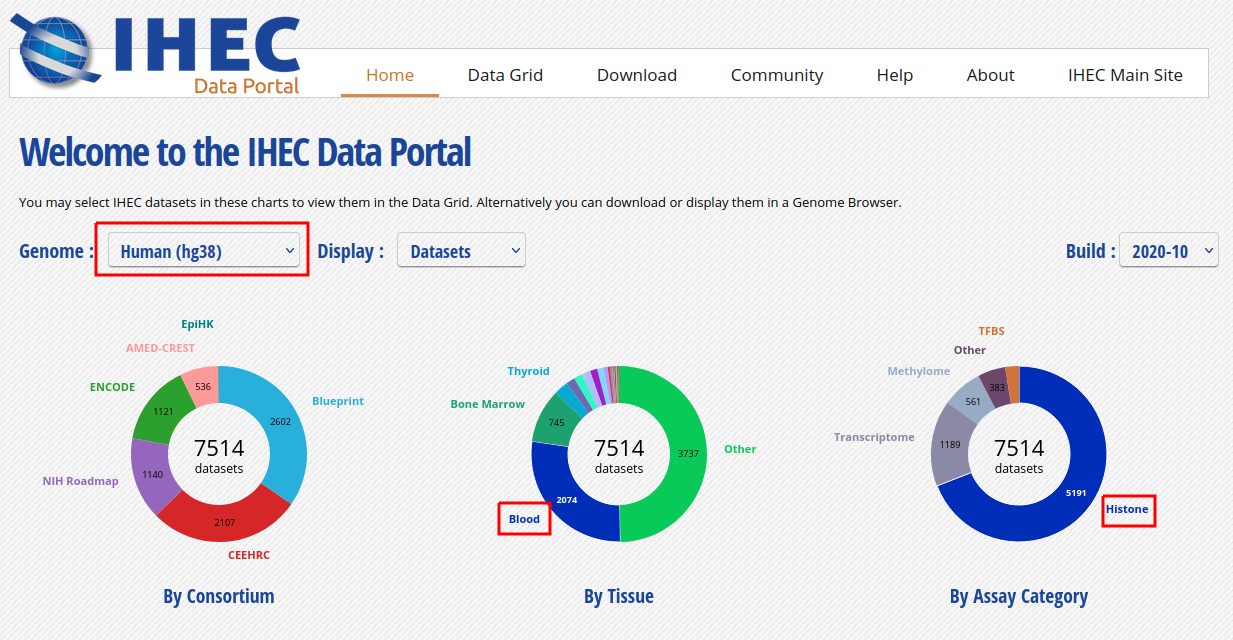
\includegraphics{./img/portal_select_from_overview.png}

\begin{itemize}
\tightlist
\item
  Only these categories will now get displayed in the grid. Expand the ``Blood'' category by clicking on the black triangle, and select the following grid cell:
\end{itemize}

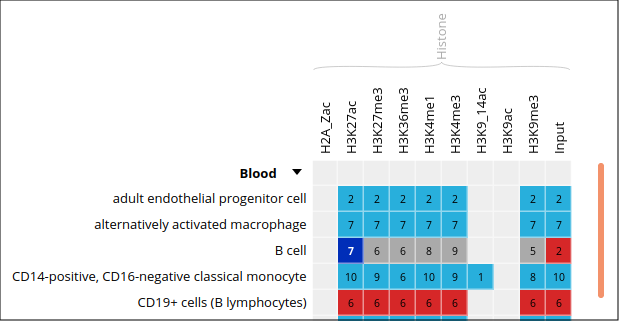
\includegraphics{./img/portal_blood_h3k27ac.png}

\subsubsection{Visualizing the Tracks}\label{visualizing-the-tracks}

\begin{itemize}
\tightlist
\item
  Click on the ``Send'' button for the UCSC Genome Browser, at the bottom of the grid
\end{itemize}

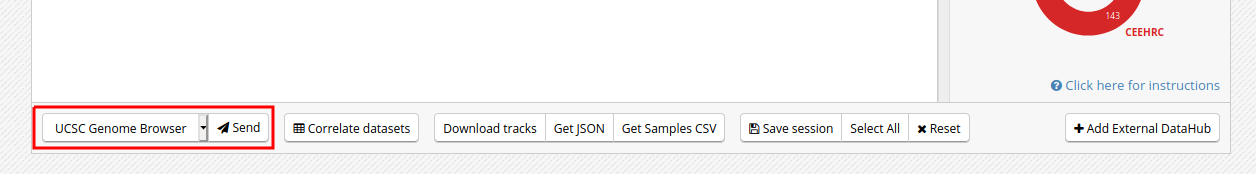
\includegraphics{./img/portal_send_to_ucsc.png}

\begin{itemize}
\tightlist
\item
  You can see that the datasets are being displayed on the UCSC Genome Browser. These are all peaks and signal for the chosen blood H3K27ac ChIP-Seq datasets. In the Genome Browser, you can expand the tracks by changing visibility from ``pack'' to ``full'' and clicking the ``Refresh'' button
\end{itemize}

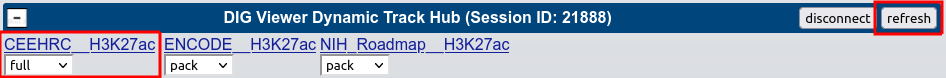
\includegraphics{./img/ucsc_fullTrackView.png}

\begin{itemize}
\tightlist
\item
  You can also download these tracks locally for visualization in IGV

  \begin{itemize}
  \tightlist
  \item
    Go back to the IHEC Data Portal tab
  \item
    Click on the ``Download tracks'' button at the bottom of the grid
  \item
    Use the download links to download a few of the available tracks
  \item
    Open them in IGV
  \end{itemize}
\end{itemize}

\subsubsection{Tracks Correlation}\label{tracks-correlation}

You can get a whole genome overview of the similarity of a group of tracks by using the Portal's correlation tool.

\begin{itemize}
\tightlist
\item
  Back on the Data Grid tab of your browser, from the filters at the right of the grid, add back datasets for all tissues and all assay types. You can select all checkboxes at once by click on the top checkbox, next to ``Category''. Also remove non-core assays if it is selected
\end{itemize}

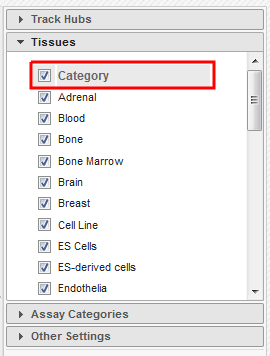
\includegraphics{./img/portal_selectAllTissues.png}

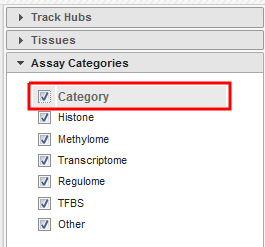
\includegraphics{./img/portal_selectAllAssays.png}

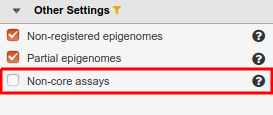
\includegraphics{./img/portal_deselect_non_core_assays.png}

\begin{itemize}
\tightlist
\item
  Select all ChIP-Seq marks for the cell type ``Myeloid cell'', under the ``Bone Marrow'' category. The first 6 columns should be selected
\end{itemize}

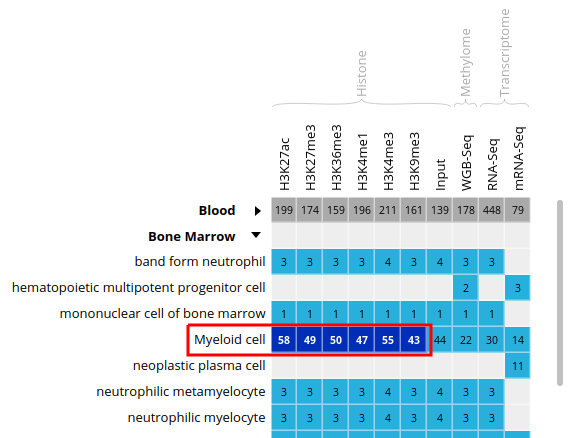
\includegraphics{./img/portal_blueprint_chipseq.png}

\begin{itemize}
\item
  At the bottom of the grid, click on the button ``Correlate datasets''
\item
  You will see that similar tracks (e.g.~those of the same assay, seem to correlate nicely. You can zoom in the view with the mouse scrolling wheel, or with the buttons at the lower right corner of the popup
\end{itemize}

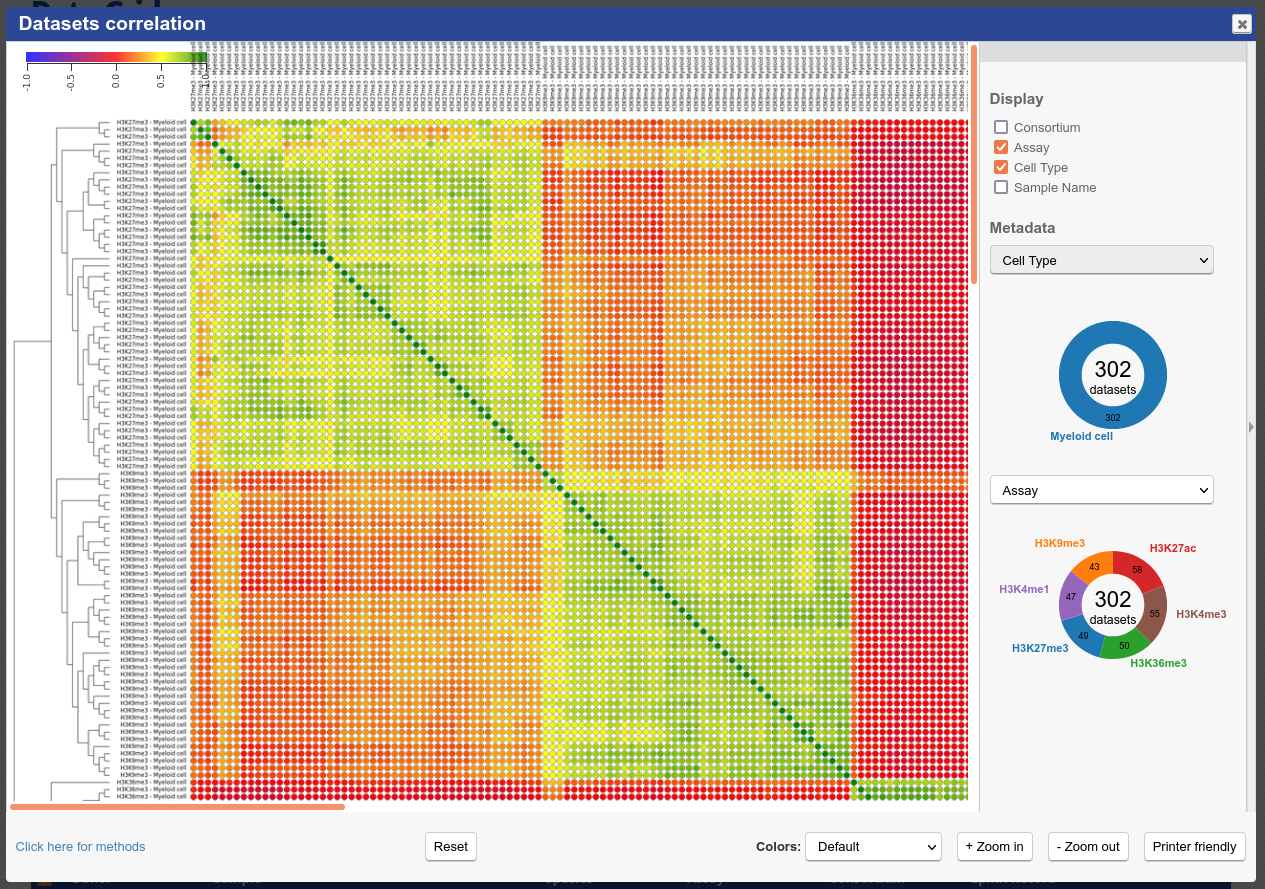
\includegraphics{./img/portal_clusteringPerMark.png}

\begin{itemize}
\tightlist
\item
  You can also use the correlation tool to assess whether datasets that are supposed to be similar actually are

  \begin{itemize}
  \tightlist
  \item
    Close the correlation popup window with the top right ``X'' button
  \item
    Reset grid selection with the ``Reset'' button at the bottom of the grid
  \item
    Click on the grid cell for cell type ``CD4-positive, alpha-beta T cell'', under the ``Blood'' category, and assay ``H3K27ac''
  \item
    Click on ``Correlate datasets''
  \item
    One dataset seems to be an outlier. This could be, for instance, a problem with the quality of the dataset, or the underlying metadata can indicate that something is different (disease status or some other key element)
  \end{itemize}
\end{itemize}

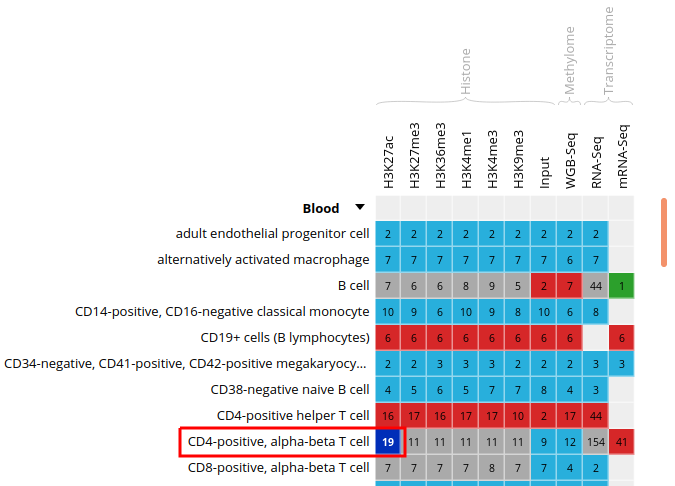
\includegraphics{./img/portal_selectTcell.png}

You should get something like this:

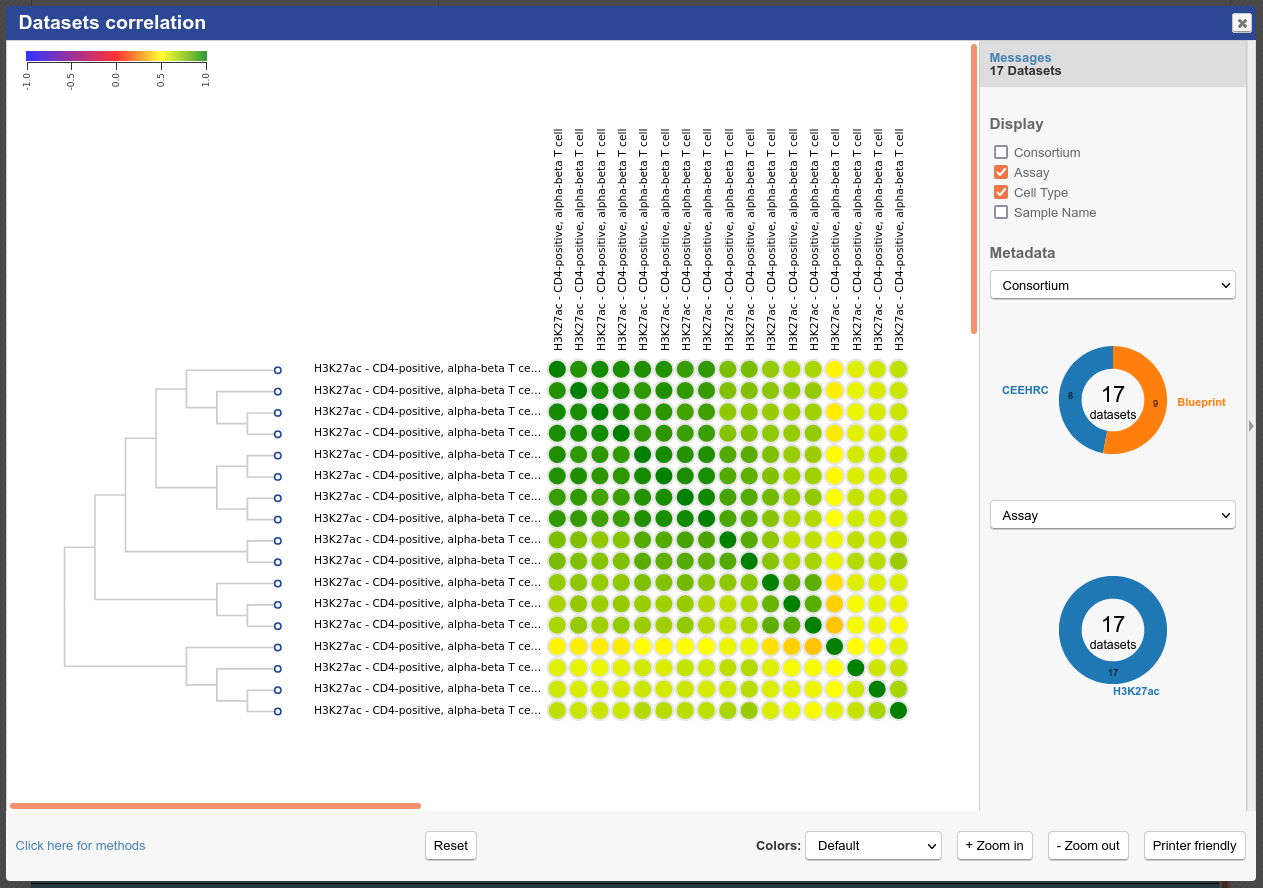
\includegraphics{./img/portal_correlationOutlier.png}

\subsection{Predicting Motifs with HOMER}\label{predicting-motifs-with-homer}

We will now attempt to detect motifs in peak regions for transcription factor binding sites using HOMER

\begin{itemize}
\tightlist
\item
  Reset to the default IHEC Data Portal view by clicking ``Data Grid'' in the top bar
\end{itemize}


\includegraphics{./img/HOMER_selectDataGrid.png}

Choose Assembly \texttt{hg19.}

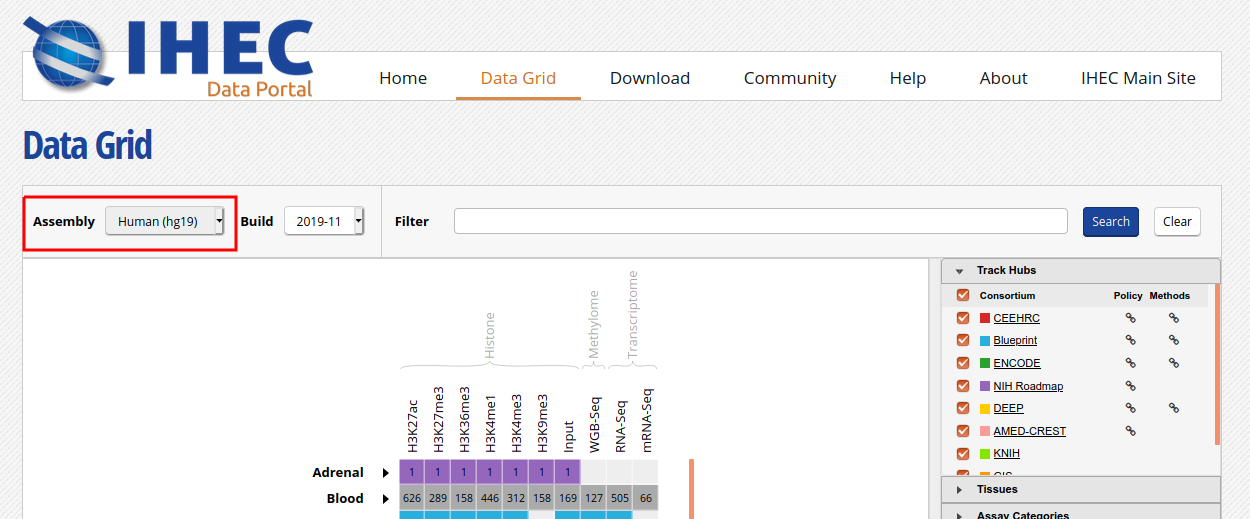
\includegraphics{./img/HOMER_selecthg19.png}

\begin{itemize}
\tightlist
\item
  In the filters to the right of the grid, activate non-core IHEC assays, and display only Transcription Factor Binding Sites (\texttt{TFBS}) assays
\end{itemize}

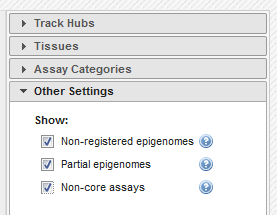
\includegraphics{./img/HOMER_showNonCoreAssays.png}

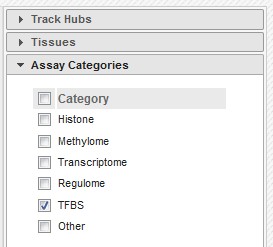
\includegraphics{./img/HOMER_showTFBS.png}

\begin{itemize}
\tightlist
\item
  In the grid, select ENCODE datasets for the \texttt{CTCF} assay and the \texttt{B\ cell} cell type
\end{itemize}

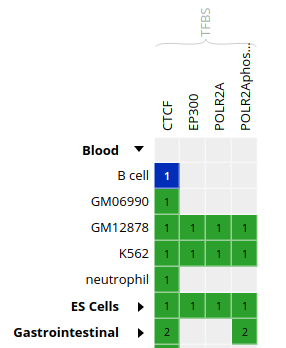
\includegraphics{./img/HOMER_selectCTCF.png}

\begin{itemize}
\tightlist
\item
  Go to the track list at the bottom of the grid and select only the dataset for sample ``ENCBS400ARI''
\end{itemize}

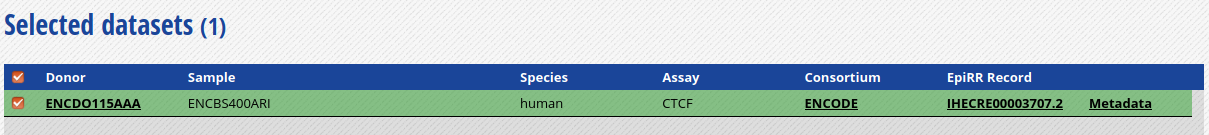
\includegraphics{./img/HOMER_selectPeaksTrack.png}

\begin{itemize}
\tightlist
\item
  You can get the URL to the track you want by clicking on the ``Download tracks'' button at the bottom of the grid Here, we're interested in \texttt{https://epigenomesportal.ca/tracks/ENCODE/hg19/84840.ENCODE.ENCBS400ARI.CTCF.peak\_calls.bigBed}. This file contains peaks that were called out of the TFBS ChIP-Seq experiment
\item
  Useful tip: You can get the full set of metadata about ENCODE experiments and samples by consulting the ENCODE portal, and searching for a given sample name. In this case: \texttt{https://www.encodeproject.org/biosamples/ENCBS400ARI/}
\item
  Open your AWS terminal session, create a directory for our HOMER-related files, and go into it. Then, download the BigBed file
\end{itemize}

\begin{verbatim}
mkdir homer
cd homer
wget https://epigenomesportal.ca/tracks/ENCODE/hg19/84840.ENCODE.ENCBS400ARI.CTCF.peak_calls.bigBed
\end{verbatim}

\begin{itemize}
\tightlist
\item
  UCSC provides a set of file format conversion tools, such as \texttt{bigBedToBed}, which converts a binary bigbed file to its plain text file equivalent. Some of these tools have been pre-installed on your AWS image
\item
  Convert the bigBed file into a bed file using the UCSC set of tools
\end{itemize}

\begin{verbatim}
bigBedToBed 84840.ENCODE.ENCBS400ARI.CTCF.peak_calls.bigBed 84840.ENCODE.ENCBS400ARI.CTCF.peak_calls.bed
\end{verbatim}

\begin{itemize}
\tightlist
\item
  Prepare an output directory for HOMER, and a genome preparsed motifs directory
\end{itemize}

\begin{verbatim}
mkdir output
mkdir preparsed
\end{verbatim}

\begin{itemize}
\tightlist
\item
  Run the HOMER software to identify motifs in the peak regions

  \begin{itemize}
  \tightlist
  \item
    -p 4 indicates to use 4 cores.
  \item
    -S 15 tells Homer to find 15 motifs, instead of the default 25, for execution speed purposes.
  \item
    You can get the full list of parameters here: \url{http://homer.ucsd.edu/homer/ngs/peakMotifs.html}
  \end{itemize}
\end{itemize}

\begin{verbatim}
findMotifsGenome.pl 84840.ENCODE.ENCBS400ARI.CTCF.peak_calls.bed hg19 output -preparsedDir preparsed -p 4 -S 15
\end{verbatim}

\begin{itemize}
\tightlist
\item
  HOMER takes a while to execute for a whole genome track like this. Expect this job to take about 30 minutes of runtime, with your current setup. In the meantime, we will explore the GO terms enrichment tool GREAT
\end{itemize}

\subsection{Looking for GO Terms Enrichment with GREAT}\label{looking-for-go-terms-enrichment-with-great}

Next, we will try to identify GO terms connected to ChIP-Seq peaks calls using GREAT. We need \texttt{bed} files to use the GREAT portal. We will do the conversion from a \texttt{bigBed} file to a \texttt{bed} file on our AWS session

\begin{itemize}
\tightlist
\item
  In the IHEC Data Portal, go back to the default grid page (by clicking on Data Grid in the top bar). For assembly \texttt{Human\ (hg38)}, filter the tissues list to keep only ``Bone Marrow'' tissues
\end{itemize}

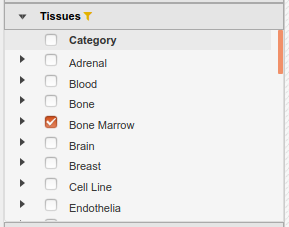
\includegraphics{./img/GREAT_select_bone_marrow.png}

\begin{itemize}
\tightlist
\item
  Select the datasets for cell type ``Myeloid cell'' and assay H3K27ac
\end{itemize}

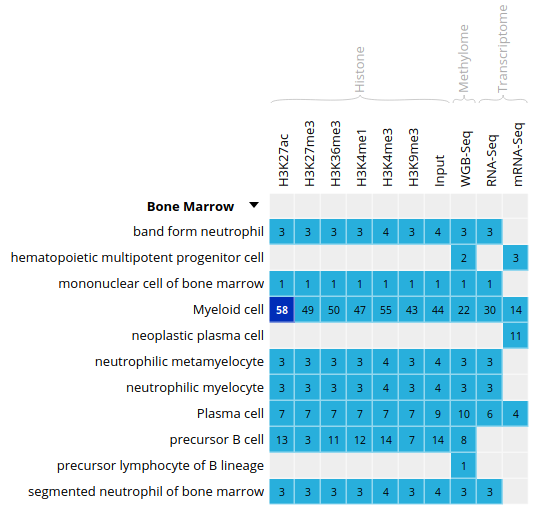
\includegraphics{./img/GREAT_bone_marrow_h3k27ac.png}

\begin{itemize}
\tightlist
\item
  For this exercise, we will download only one of the bigbeds for available datasets. Pick up the dataset below, for sample \texttt{ERS1027405}:
\end{itemize}

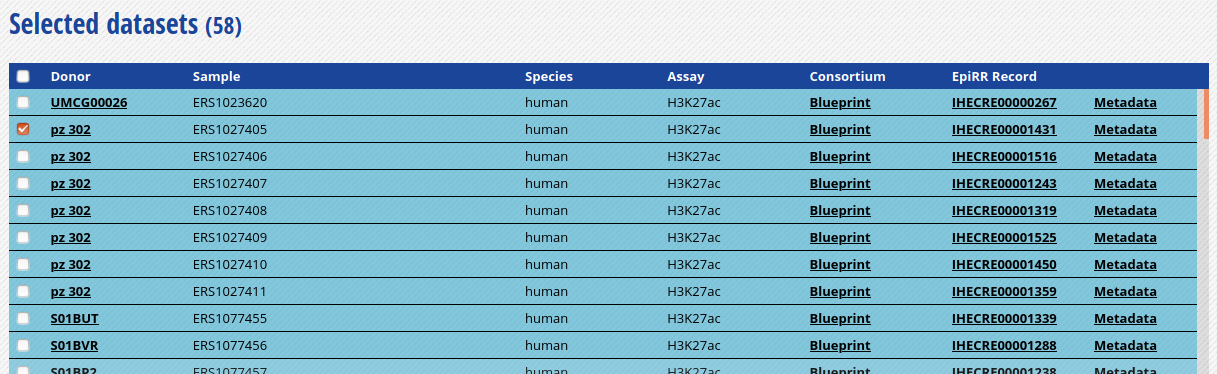
\includegraphics{./img/GREAT_selectSomeBoneMarrowDatasets.png}

\begin{itemize}
\item
  Click ``Download tracks'' at the bottom of the grid
\item
  On the download page, click on \texttt{View\ Full\ URL\ List}. This will give you a text list with all tracks of interest Copy the link to this page in your clipboard, using the address provided in your browser's URL bar
\end{itemize}

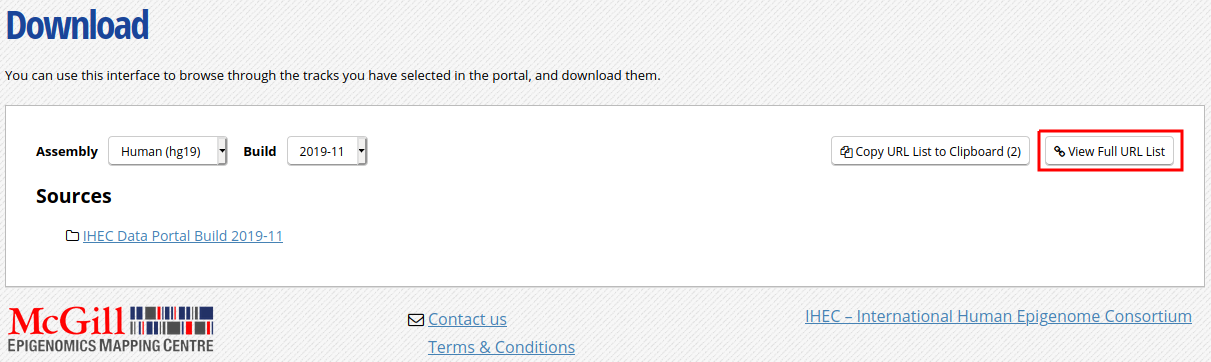
\includegraphics{./img/GREAT_batch_download.png}

\begin{itemize}
\item
  Open another terminal session to get into AWS
\item
  Go to your module5 directory and create a place to put the material we will download
\end{itemize}

\begin{verbatim}
cd ~/workspace/module5
mkdir great
cd great
\end{verbatim}

\begin{itemize}
\tightlist
\item
  For you own analyses, you can download a bunch of tracks at the same time by using wget on a list of URLs

  \begin{itemize}
  \tightlist
  \item
    Use the \textbf{wget} command to download the text file that contains the list of tracks
  \end{itemize}
\end{itemize}

\begin{verbatim}
wget -O trackList.txt 'https://epigenomesportal.ca/api/datahub/download?session=18731&format=text'
\end{verbatim}

\begin{itemize}
\tightlist
\item
  Now download the tracks that are contained in this list
\end{itemize}

\begin{verbatim}
wget -i trackList.txt
\end{verbatim}

\begin{itemize}
\tightlist
\item
  Convert the bigbed using the UCSC set of tools
\end{itemize}

\begin{verbatim}
bigBedToBed 58394.Blueprint.ERS1027405.H3K27ac.peak_calls.bigBed 58394.Blueprint.ERS1027405.H3K27ac.peak_calls.bed
\end{verbatim}

If you're under Linux / Mac, you can also install the UCSC tools locally, as they are a useful set of tools to manipulate tracks data, without requiring so much processing power.

\begin{itemize}
\tightlist
\item
  GREAT has a limit on the number of regions to be tested in one execution. Therefore, we need to subsample our file. We can create a BED file subsample this way:

  \begin{itemize}
  \tightlist
  \item
    Sort BED file in random order with \texttt{sort\ -R}
  \item
    Take the 20000 first lines in the file with head \texttt{-n20000}
  \end{itemize}
\end{itemize}

\begin{verbatim}
sort -R 58394.Blueprint.ERS1027405.H3K27ac.peak_calls.bed > 58394.Blueprint.ERS1027405.H3K27ac.peak_calls.random.bed
head -n 20000 58394.Blueprint.ERS1027405.H3K27ac.peak_calls.random.bed > 58394.Blueprint.ERS1027405.H3K27ac.peak_calls.random_short.bed
\end{verbatim}

\begin{itemize}
\tightlist
\item
  From your local computer, download the BED file \texttt{58394.Blueprint.ERS1027405.H3K27ac.peak\_calls.random\_short.bed} locally using your browser
\end{itemize}

\begin{verbatim}
http://<your VM ip address>/module5/great/58394.Blueprint.ERS1027405.H3K27ac.peak_calls.random_short.bed
\end{verbatim}

\begin{itemize}
\item
  Load the GREAT website: \url{http://bejerano.stanford.edu/great/public/html/}
\item
  Provide the following input to the GREAT interface:

  \begin{itemize}
  \tightlist
  \item
    Assembly: Human: GRCh38
  \item
    Test regions: The randomized short version of the BED files you just downloaded (58394.Blueprint.ERS1027405.H3K27ac.peak\_calls.random\_short.bed)
  \item
    Leave the ``Background regions'' to its default value, ``Whole Genome''
  \end{itemize}
\item
  Submit the form
\item
  In the results, for instance, you should obtain something like this for biological processes:
\end{itemize}

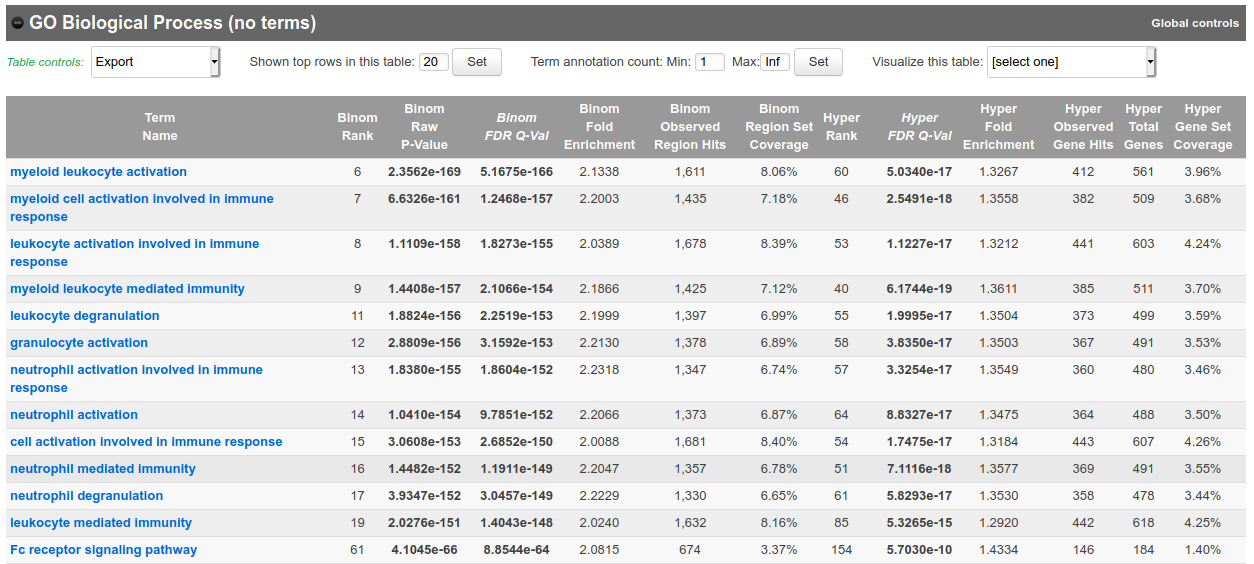
\includegraphics{./img/GREAT_go_biological_process.png}

Bonus question: Why is your result slightly different from the screenshot?

\subsection{Going back to HOMER Results}\label{going-back-to-homer-results}

\begin{itemize}
\tightlist
\item
  Is the job done? If it is completed, you can bring back HOMER results to your laptop for visualization. First we'll compress the results to a zip file
\end{itemize}

\begin{verbatim}
cd ~/workspace/module5/homer/
zip -r homer.zip output
\end{verbatim}

\begin{itemize}
\tightlist
\item
  Next, with your web browser, download the zipped result set
\end{itemize}

\begin{verbatim}
http://<your VM ip address>/module5/homer/homer.zip
\end{verbatim}

\begin{itemize}
\tightlist
\item
  Unzip the file, and open the de novo and known motifs HTML files in a browser for visualization. Do the identified motifs fit what we would expect?
\end{itemize}

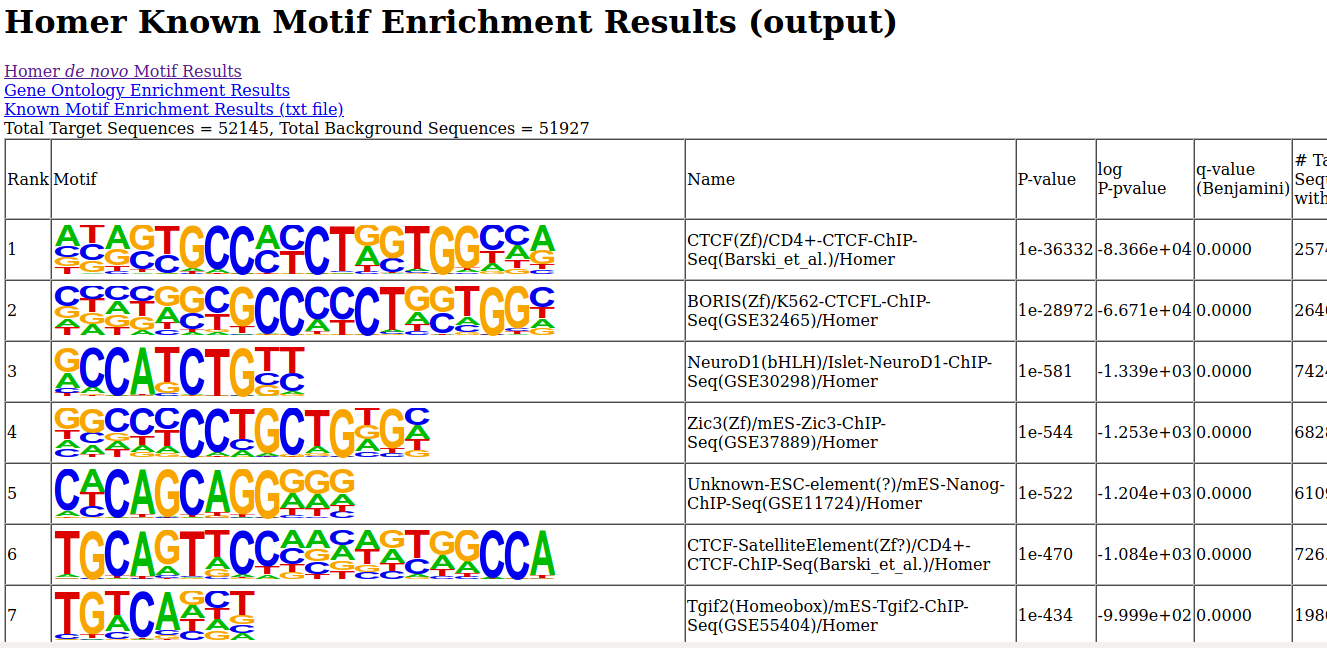
\includegraphics{./img/HOMER_results.png}

\subsubsection{All done!}\label{all-done}

If you have time remaining, you can explore further the tools that we covered in this lab, using other types of datasets. For example, does running a GREAT query on another cell type yield the type of annotations that you'd expect?

\textbf{Interested in exploring Galaxy?} You can start tackling a Galaxy introduction extra lab, available \href{https://bioinformaticsdotca.github.io/EPI_2023_module5_galaxy}{here}. It uses the usegalaxy.org server, so you can also follow it at your own pace after the workshop.

Congratulations! You have completed Lab 5!

  \bibliography{book.bib,packages.bib}

\end{document}
